
\documentclass[10pt]{report}

\usepackage{csquotes}
\usepackage{graphicx}
\usepackage{color}
\usepackage[spanish]{babel}
\usepackage{amsmath,amsfonts,amssymb,amsthm}
\usepackage{fontenc,url,path}
\usepackage{hyperref}
\usepackage{float}
\usepackage{bookmark}
\usepackage{todonotes}

\usepackage{geometry} % Add this line
\geometry{margin=1.4in} % Adjust margins as needed

\usepackage{biblatex} %Imports biblatex package
\addbibresource{referencias.bib}

\hypersetup{colorlinks,
            urlcolor=blue,
            citecolor=blue}

\graphicspath{{figuras/}}

% layout pars
\setlength{\parindent}{0pt}
\setlength{\arraycolsep}{2pt}
\setlength{\parskip}{3pt}
\vfuzz2pt % don't report over-full v-boxes if over-edge is small
\hfuzz2pt % don't report over-full h-boxes if over-edge is small

% commands
\newcommand{\intro}[1]
  {{\normalsize\textsf{#1}}}

\newcommand{\blankpage}%
  {\newpage
   \null\vfill\eject}

% customized 'description' environment
\renewcommand{\descriptionlabel}[1]%
	{\hspace{\labelsep}\textsf{#1}}

% text commands
\def\etal{et al.}
\def\ie{i.e}
\renewcommand\spanishtablename{Tabla}

% math commands
\DeclareMathOperator{\E}{E}
\DeclareMathOperator{\Cov}{Cov}
\DeclareMathOperator{\Cor}{Cor}
\DeclareMathOperator{\var}{var}
\DeclareMathOperator{\abs}{abs}
\DeclareMathOperator{\argmax}{arg\,max}
\DeclareMathOperator{\argmin}{arg\,min}
\DeclareMathOperator{\blkdiag}{blc\,diag}
\DeclareMathOperator{\diag}{diag}
\DeclareMathOperator{\rd}{d}
\DeclareMathOperator{\GIF}{GIF}
\let \max \relax
\DeclareMathOperator{\max}{max}
\let \min \relax
\DeclareMathOperator{\min}{min}
\DeclareMathOperator{\nullity}{nulidad}
\let \Pr \relax
\DeclareMathOperator{\Pr}{P}
\DeclareMathOperator{\rk}{rg}
\let \SS \relax
\DeclareMathOperator{\SS}{SS}
\DeclareMathOperator{\SSD}{SSD}
\DeclareMathOperator{\tr}{tr}
\let \vec \relax
\DeclareMathOperator{\vec}{vec}
\DeclareMathOperator{\vech}{vech}
\DeclareMathOperator{\vecp}{vecp}
\def\half{{\textstyle\frac{1}{2}}}
\def\Cset{\mathbb{C}}
\def\Hset{\mathbb{H}}
\def\Nset{\mathbb{N}}
\def\Qset{\mathbb{Q}}
\def\Rset{\mathbb{R}}
\def\Zset{\mathbb{Z}}
\def\D{\mathsf{D}}
\def\H{\mathsf{H}}
\newcommand{\bt}[1]{\ensuremath{\mathbf{#1}}}  % bold text
\newcommand{\bm}[1]{\mbox{\boldmath $#1$}}     % bold math
\newcommand{\bc}[1]{\ensuremath{\mathcal{#1}}}  % bold text
\newcommand{\what}[1]{\widehat{#1}}             % shortcut for \widehat
\newcommand{\C}{\textsf{C}}
\newcommand{\Fortran}{\textsc{Fortran}}
\newcommand{\R}{\mathbb{R}}
\newcommand{\s}{\textsf{S}}
\newcommand{\Splus}{\textsc{S-Plus}}

% Theorems -------------------------------------------------------------
\theoremstyle{plain}
\newtheorem{fact}{Hecho}
\newtheorem{thm}{Teorema}[chapter]
\newtheorem{cor}[thm]{Corolario}
\newtheorem{lem}[thm]{Lema}
\newtheorem{property}[thm]{Propiedad}
\theoremstyle{definition}
\newtheorem{defn}{Definici\'{o}n}[chapter]
\newtheorem{asump}{Supuesto}[chapter]
\newtheorem{prop}{Proposici\'{o}n}[chapter]
\newtheorem{result}{Resultado}[chapter]
\theoremstyle{remark}
\newtheorem{rem}{Observaci\'{o}n}[chapter]
\newtheorem{example}{Ejemplo}[chapter]

\title{{\LARGE\textbf{T\'opicos de Modelaci\'on Estad\'istica}} \\[0.8ex]
    {\large\textbf{Notas de Clase MAT-305: M\'etodos Estad\'isticos}}}

\author{Felipe Osorio}

\hyphenation{ob-te-ne-mos
    pro-ba-bi-li-dad
    si-guien-tes
    va-rian-za}

\begin{document}

\DeclareGraphicsExtensions{.epsi.gz,.epsi,.eps.gz,.eps,.ps,.ps.gz}

% ----------------------------------------------------------------------

% ---------------------------------------------------------------------------------------
\thispagestyle{empty}

\begin{center}
%~\\
%~\\
\large \textbf{UNIVERSIDAD T\'ECNICA FEDERICO SANTA MAR\'IA}

\vspace{3mm}

\normalsize DEPARTAMENTO DE MATEM\'ATICA
\vspace{35mm}

\Large {\bf An\'alisis de Im\'agenes a trav\'es de la Transformaci\'on de Box-Cox}

\vspace{35mm}

\normalsize Memoria de T\'itulo presentada por

\vspace{2mm}

\large{\textbf{Fabi\'an Castellano N\'u\~nez}}

\vspace{10mm}

\normalsize como requisito parcial para optar al t\'itulo de

\vspace{2mm}

\textbf{Ingeniero Civil Matem\'atico}

\vspace{15mm}

Profesor Gu\'ia

\vspace{2mm}

Dr. Ronny Vallejos A.

\vspace{5mm}

Marzo, 2024.

\end{center}
\blankpage
\chapter*{Agradecimientos.}

Primero que todo, debo agradecer a las dos m\'ujeres m\'as importantes de mi vida, mi madre Jessicca y mi pareja Noem\'i, sin su amor y apoyo incondicional me hubiera sido imporsible llegar tan lejos. No hay palabras que pueda escribir para expresar todo lo que les debo.

Junto con ellas debo mencionar a mi Lela Rosa, a quien no llamo por telefono tanto como deber\'ia, pero siempre esta presente cuandio m\'as la necesito.

Gracias a mis amigos, en particular a Gustavo, Bruno, y Ricardo, por siempre estar disponibles para ayudar, y recordarme que el final no está tan lejos. 

Agradezco tambi\'en a mi profesor gu\'ia, Dr. Ronny Vallejos, no solo por el apoyo y la direcci\'on que me dió durante el trabajo, sino por la gran cantidad paciencia y cariño que me entreg\'o durante todo el proceso. 

No puedo olvidar dar las gracias a la gente de TallerCaf\'e; Gabriela, Camilo, y Monserrat, por siempre estar para entregar animos, y por aguantar mis quejas sobre este trabajo por m\'as tiempo de el que me es c\'omodo admitir.

Por \'ultimo, agradezco al mi familia, que a pesar de la distancia su apoyo es sentido y apreciado.
% show outile 
\setcounter{tocdepth}{1}
\tableofcontents
\blankpage
% ---------------------------------------------------------------------------------------
\chapter{Introducci\'on}\label{chap1}

En el an\'alisis de datos, es com\'un verse enfrentado con datos problem\'aticos, valores faltantes, datos at\'ipicos, o datos que no distribuyan de forma normal. Para el \'ultimo caso es com\'un aplicar transformaciones a los estos para que su distribuci\'on se asemeje a una Normal. Una de las transformaciones m\'as comunes para lograr esto es la transformaci\'on de Box-Cox, la cual busca a travez de un problema de optimizaci\'on, encontrar el valor de $\lambda$ que mejor ajuste los datos a una distribuci\'on Normal. Esta transformaci\'on suele aplicase sobre  vectores unidimensionales, y no ha sido extendida a matrices $d$-dimensionales en las que existe corrlaciones de adyacencia, excepto en una cantidad muy reducida de trabajos, en los que destacan Lee et. al. \textit{(MR Image Segmentation Using a Power Transformation Approach)}\cite{lee2009mr}, y Bicego y Baldo \textit{(Properties of the Box-Cox Transformation for Pattern Classification)}\cite{bicego2016}. 

En el primero se trata el problema de segmentaci\'on de imagenes de resonancia magn\'etica, y utlizan la transformaci\'on simplemente aplananado la matriz de la imagen. En el segundo se estudian distintas propiedes de la transformaci\'on de Box-Cox sobre ima\'agenes, en particular para clasificaci\'on de patrones. En el segundo trabajo, se propone algo interesante, utilizar el histograma de la imagen para encontrar el valor de $\lambda$ que mejor ajuste los valores de este a una distribuci\'on normal. Dado este interes por aplicar la transformaci\'on de Box-Cox a im\'agenes, y la falta de trabajos en esta direcci\'on, nos interesa estudiar la relaci\'on que existe entre la transformaci\'on de Box-Cox y la im\'agen original de donde proviene,

Recordemos que esta transformaci\'on es no lineal, por lo que nos interesa utilziar m\'etodos de comparaci\'on que nos permitan detectar relaciones no lineales entre las variables. Por esto es que comenzaremos el trabajo en el Cap\'itlo \ref{chap2} dos m\'etodos de comparaci\'on: \textit{Maximal Information Coefficient} o MIC, y \textit{Distance Correlation} o dCor. Revisaremos como se define cada uno, y como podemos calcularlo, adem\'as de algunos ejemplos de su aplicaci\'on.

Continuaremos en el Cap\'itlo \ref{chap3} revisando como trabajamos con im\'agenes, su interpretaci\'on como matrices, y como procederemos a aplicar m\'etodos de comparaci\'on sobre estas imagenes. Adem\'as revisaremos el banco de imagenes que utilizaremos para realizar los experimentos. En este cap\'itulo tambi\'en discutiremos como podemos aplicar los m\'etodos de correlaci\'on estudiados en el cap\'itulo \ref{chap2} sobre im\'agenes.

Luego, en el Cap\'itlo \ref{chap4} procederemos a estudiar la tranformaci\'on de Box-Cox, su definici\'on, como podemos aplicarla sobre im\'agenes, y discutiremos distintos m\'etodos para la obtenci\'on del valor $\lambda$. 

Finalmente en el Cap\'itlo \ref{chap5}procederemos a realizar experimentos num\'ericos, en los que aplicaremos la transformaci\'on de Box-Cox sobre im\'agenes, y compararemos la im\'agen original con la transformada, estudiaremos tanto la relaci\'on para un rango de valores de $\lambda$, como para distintos m\'etodos de obtenci\'on de $\lambda$.

El objetivo de este trabajo es estudiar la relaci\'on que existe entre la transformaci\'on de Box-Cox y la im\'agen original de donde proviene, en particular para distintas formas de encontrar valores de $\lambda$, y para distintos tipos de im\'agenes. Adem\'as de proponer un m\'etodo para encontrar el valor de $\lambda$. Junto con esto, tambie\'en se explora el concepto de comparaci\'on de ima\'agenes, proponiendo un m\'etodo novedoso para comparar im\'agenes que no se basa en la comparaci\'on de pixeles, sino que en la comparaci\'on de la distribuci\'on de los valores de los pixeles, utilizando el histograma de la imagen como base para la comparaci\'on.
\blankpage
\chapter{Coeficientes de Correlaci\'on}\label{chap2}
    \section{Introducción}
        \todo{hacer intro del capitulo}

    \section{\textit{Maximal Information Coeficient}}\label{chap2}

    \subsection{Introducci\'on}
    
    El Coeficiente de Informaci\'on m\'axima (conocido como MIC por sus siglas en ingl\'es), es una medida estad\'istica propuesta por Reshef et al. en su trabajo "Detecting Novel Associations in Large Data Sets" \cite{Reshef2011}. Este coeficiente fue creado en el contexto de la ciencia generadora de hip\'otesis, en la cual los conjuntos de datos se utilizan para ayudar a los investigadores a formular nuevas hip\'otesis en lugar de probar las existentes. En este enfoque, se utilizan medidas de dependencia, que son estad\'isticas empleadas para evaluar pares de variables candidatas. Estos avances en el campo de analisis de datos nos han entregado muchas herramientas, tanto para la comparaci\'on de datos en si mismos, junto con formas de evaluar estas medidas en si mismas.
    
    Sea $\hat\varphi$ una medida de dependencia, una forma de medir la utilidad de esta es la \textit{potencia contra la independencia}, i.e., la capacidad de prueba de independencia basada en $\hat\varphi$ para detectar varios tipos de relaciones no triviales. Este es un objetivo importante para conjuntos de datos que tienen muy pocas relaciones no triviales, o solo relaciones muy d\'ebiles que son dif\'iciles de detectar. Sin embargo, a menudo el n\'umero de relaciones declaradas estad\'isticamente significativas por una medida de dependencia supera con creces el n\'umero de relaciones que luego se pueden explorar m\'as a fondo.
    
    Para abordar este problema, se introdujo un segundo m\'etodo de evaluaci\'on de una medida de dependencia llamado equitabilidad \cite{Reshef2011}. Las estad\'isticas equitativas asignan puntuaciones similares a relaciones igualmente fuertes, independientemente de su tipo. El objetivo es definir medidas de dependencia que logren una buena equitabilidad con respecto a medidas relevantes de la fuerza de la relaci\'on. 
    
    La idea de equitabilidad ha motivado el desarrollo de varias medidas de dependencia, con diferentes formalizaciones y enfoques en aspectos espec\'ificos de la fuerza de la relaci\'on. El desaf\'io radica en definir medidas de dependencia que logren una buena equitabilidad con respecto a medidas importantes de la fuerza de la relaci\'on, como se ve en el art\'iculo complementario de Reshef et al (2011) \cite{Reshef2011}. Esta l\'inea de investigaci\'on tiene como objetivo proporcionar un enfoque m\'as poderoso y equitativo para medir la dependencia, lo que permite una identificaci\'on y priorizaci\'on m\'as precisas de las relaciones en conjuntos de datos complejos.
    
    En este contexto, el coeficiente de informaci\'on m\'axima (MIC) nos entrega una medida rebusta para encontrar relaci\'ones no lineales entre variables, para nuestro caso en particular, entre im\'agenes. C\'omo veremos en la secci\'on \ref{chap5}, la transformaci\'on de Box-Cox es no lineal, por lo que el coeficiente nos ayudar\'a a cuantificar la relaci\'on entre las im\'agenes transformadas y las originales, y podemos aprovechar la equitabilidad de este para comparar diferentes versiones de la transformaci\'on.
    
    En esta secci\'on discuteremos la definici\'on del MIC, algunas de sus propiedades y un par de caracterizaciones que nos ayudar\'an a llegar al $MIC_*$ y posteriormente al $MIC_e$, ambos siendo estimadores de $MIC$ que nos har\'an posible calcular este valor. 
    
    \subsection{Sobre el coeficiente}
    
        El coeficiente de informaci\'on m\'axima (Maximal Information Coefficient o MIC) es una medida estad\'istica propuesta por Reshef et al. en su paper "Detecting Novel Associations in Large Data Sets" \cite{Reshef2011}. Este coeficiente mide la correlaci\'on entre dos variables en un conjunto de datos y se basa en la idea de que una relaci\'on fuerte entre dos variables deber\'ia ser capaz de predecir una variable a partir de la otra de manera precisa.
    
        En este paper, Reshef et al. presentan un enfoque innovador para detectar asociaciones nobles en grandes conjuntos de datos, en lugar de buscar correlaciones fuertes entre dos variables, el coeficiente MIC permite detectar relaciones d\'ebiles pero a\'un importantes que pueden no ser evidentes al simplemente mirar los datos. Esto es posible gracias a que el coeficiente MIC es capaz de capturar no solo la fuerza de la correlaci\'on entre dos variables, sino tambi\'en su precisi\'on.
    
        Para calcular el coeficiente, se comienza de la idea de que la informaci\'on mutua entre dos variables es una medida de la precisi\'on con la que se puede predecir una variable a partir de la otra. Por lo tanto, el coeficiente se calcula como la informaci\'on mutua m\'axima posible entre dos variables, dado un conjunto de datos. Esto se hace a trav\'es de un procedimiento iterativo en el que se prueban diferentes particiones de los datos en conjuntos de entrenamiento y prueba, y se selecciona aquella que maximiza la informaci\'on mutua.
    
        El la siguiente secci\'on estudiaremos las definiciones que nos entrega cada coeficiente.
     
    \subsection{Definiciones}
    
        Como mencionamos en la parte anterior, debemos primero encontrar la informaci\'on mutua entre las variables.
    
        \begin{defn}[Informaci\'on mutua]
            Para un vector aleatorio bivariado $(X,Y)$, se define la informaci\'on mutua como:
            $$
            \mathrm{I}(X ; Y)=\int_{\mathcal{Y}} \int_{\mathcal{X}} P_{(X, Y)}(x, y) \log \left(\frac{P_{(X, Y)}(x, y)}{P_{X}(x) P_{Y}(y)}\right)dxdy,
            $$
            donde $P_{(X, Y)}$ es la funci\'on de densidad de probabilidad conjunta y $P_{X}$, $P_{Y}$, las distribuciones marginales de $X$ e $Y$ respectivamente. 
        \end{defn}
    
        Luego, sea $D$ un conjunto finito de pares ordenados, podemos particionar los valores de la primera coordenada en $x$ contenedores, y los valores de la segunda en $y$ de estos. Dado una malla $G$, sea $D|_G$ la distribuci\'on inducida por los puntos de $D$ en las celdas de $G$, i.e., la distribuci\'on en las celdas de $G$ obtenida al dejar que la funci\'on de densidad de probabilidad en cada celda sea la fracci\'on de puntos de $D$ que caen en esa celda. Veamos un ejemplo
        \begin{figure}[H]
            \centering
            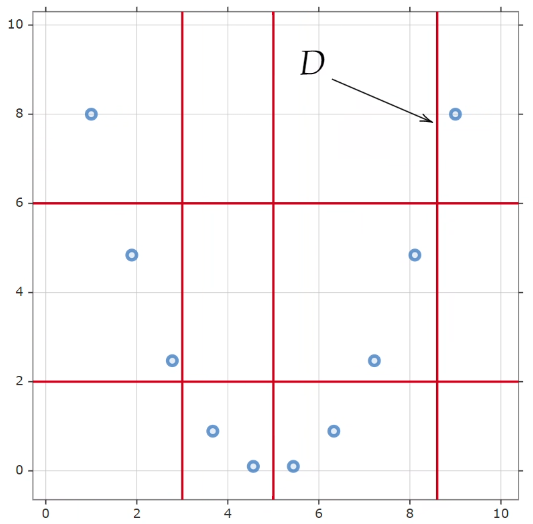
\includegraphics[scale = 0.4]{mallaG4x3.png}
            \caption{Malla G de 4x3 sobre el conjunto de pares ordenados D}
            \label{mallaG}
        \end{figure}
    
        Para la Figura \ref{mallaG}, la funci\'on de densidad quedar\'ia de la forma:
        \[
            f_{D|_G}(i,j) = \left\{\begin{array}{lr}
                \frac{1}{10} & \text{si } (i,j) \in \{ (1,3), (4,1)\} \\
                \frac{2}{10}, & \text{si }(i,j) \in \{ (1,2), (2,1), (3,1),(3,2)\}  \\
                0, & \text{Otro caso.}
                \end{array}\right.
        \]
    
    
    
        Notemos que para un $D$ fijo, aunque fijemos el grosor de la malla, la distribuci\'on de esta puede variar dependiendo de donde hagamos los cortes, por ejemplo:
    
        \begin{figure}[H] 
            \centering
            \includegraphics*[scale = 0.4]{mallaG4x3_2.png}
            \caption{Otra malla G de 4x3 sobre el conjunto de pares ordenados D.}
            \label{malla_G_2}
        \end{figure}
    
        Aqu\'i podemos ver que la funci\'on de densidad que nos entrega est\'a malla es distinta a la definida para la Figura \ref{malla_G_2} . Este es un hecho que explotamos en la siguiente definici\'on: 
    
        \begin{defn}
            Para un conjunto finito $D\in\R^2$ y enteros positivos $i,j$, definimos:
            $$
            I^*(D,i,j)=\max I(D|_G),
            $$
            donde el m\'aximo es sobre todas las mallas $G$ con $i$ columnas y $j$ filas, con $I(D|_G)$ denota la informaci\'on mutua de $D|_G$.
        \end{defn}
    
        Ya teniendo este valor procedemos a definir la matriz caracteristica del conjunto $D$.
    
        \begin{defn}
            La matriz caracteristica $M(D)$ de un conjunto de pared ordenados $D$ es una matriz infinita con entradas:
            $$
            M(D)_{x, y}=\frac{I^{*}(D, x, y)}{\log \min \{x, y\}}.
            $$
        \end{defn}
        \begin{defn}
            El coeficiente de informaci\'on m\'axima o \textit{MIC} de un conjunto bivariado $D$ de tama\~no $n$ y una malla de tama\~no menor a $B(n)$ esta dado por:
    
            $$
            \operatorname{MIC}(D)=\max _{x y<B(n)}\left\{M(D)_{x, y}\right\},
            $$
    
            donde $\omega(1)<B(n) \leq O\left(n^{1-\varepsilon}\right)$ para alg\'un $0<\varepsilon<1$.
        \end{defn}
        \begin{rem}
            A menos que se especifique de otra forma, al momento de trabajar con esta medida usaremos $B(n)=n^{0.6}$, funci\'on de la cu\'al se encontr\'o que funcon\'a en pr\'actica en el art\'iculo complementario de Reshef et al. (2011) \cite[]{Reshef2011}, discuteremos la selecci\'on de este par\'ametro m\'as adelante en \ref{eligiendo_Bn}
        \end{rem}
    
    
        \subsection[Formas practicas de calcular el MIC. MIC*, TICe y MICe]{Formas pr\'acticas de calcular el $MIC$. $MIC_*$, $TIC_e$ y $MIC_e$}
    
        En el art\'iculo "Measuring Dependence Powerfully and Equitably" de Reshef et al. \cite{Reshef2016}, los autores presentan y caracterizan te\'oricamente dos nuevas medidas de dependencia: $MIC_*$ y $MIC_e$. $MIC_*$ es una medida de dependencia poblacional, y el art\' iculo presenta tres formas de ver esta cantidad. Los autores demuestran que $MIC_*$ es el valor poblacional del coeficiente de informaci\'on m\'axima (MIC), una suavizaci\'on m\'inima de la informaci\'on mutua y el supremo de una secuencia infinita. Estas caracterizaciones simplifican el c\'alculo y fortalecen los resultados te\'oricos.
    
        Adem\'as, los autores desarrollan algoritmos eficientes para aproximar $MIC_*$ en la pr\'actica y estimarlo de manera consistente a partir de una muestra finita. Introducen $MIC_e$, un estimador consistente de $MIC_*$, que es computable de manera eficiente y m\'as r\'apido en la pr\'actica que el algoritmo heur\'istico para calcular MIC. A trav\'es de simulaciones, demuestran que $MIC_e$ tiene mejores propiedades de sesgo/varianza y supera a los m\'etodos existentes en t\'erminos de equitabilidad con respecto a R2 en un amplio conjunto de relaciones funcionales ruidosas.
    
        \subsubsection[short]{Definiciones y propiedades de $MIC_*$}
    
        En esta secci\'on, abordaremos las definiciones esenciales para el c\'alculo del $MIC_e$. El coeficiente m\'aximo de informaci\'on poblacional puede expresarse de diversas maneras equivalentes, como veremos m\'as adelante. Sin embargo, comenzaremos con la definici\'on m\'as sencilla.
    
        \begin{defn}
            Sea $(X,Y)$ un vector aleatorio bivariado. El coeficiente de informaci\'on m\'axima poblacional ($MIC_*$) de $(X,Y)$ se define como:
            $$
            M I C_*(X, Y)=\sup _G \frac{I\left(\left.(X, Y)\right|_G\right)}{\log \|G\|},
            $$
            
            donde $||G||$ denota el m\'inimo entre el n\'umero de filas y el n\'umero de columnas de la malla $G$.
        \end{defn}
        
        Ya que $I(X,Y) = sup_G I((X,Y)|G)$ (Cover y Thomas, 2006 \cite[Cap. 8]{CoverThomas2006}), esto puede interpretarse como una versi\'on regularizada de la informaci\'on mutua que sanciona las rejillas complejas y garantiza que el resultado est\'e dentro del rango entre cero y uno.
        
        Previo a continuar, introducimos una definici\'on equivalente y sencilla de $MIC_*$ que resulta \'util para los resultados en esta secci\'on. Esta definici\'on considera a $MIC_*$ como el supremo de una matriz denominada matriz caracter\'istica poblacional, que se define a continuaci\'on.
        
        \begin{defn}
            Sea $(X,Y)$ una pareja de variables aleatorias conjuntamente distribuidas. Sea
            $$
            I^*((X, Y), k, \ell)=\max _{G \in G(k, \ell)} I\left(\left.(X, Y)\right|_G\right),
            $$
            la matriz caracter\'istica poblacional de (X,Y), denotada por M(X,Y), se define como
            $$
            M(X, Y)_{k, \ell}=\frac{I^*((X, Y), k, \ell)}{\log \min \{k, \ell\}}.
            $$
        \end{defn}
        
        para $k$, $l > 1$.
        
        Es f\'acil ver lo siguiente:
    
        \begin{prop}
            Sea $(X,Y)$ una vector aleatorio bidimensional de variables aleatorias conjuntamente distribuidas. Tenemos
        
        $$MIC_*(X,Y) = \sup M(X,Y),$$
        
        donde $M(X,Y)$ es la matriz caracter\'istica poblacional de $(X,Y)$.
        \end{prop}	
    
        
        La matriz caracter\'istica poblacional recibe este nombre porque, al igual que el $MIC_*$, el supremo de esta matriz, captura una noci\'on de la intensidad de la relaci\'on, y otras propiedades de esta matriz se relacionan con diferentes caracter\'isticas de las relaciones. Por ejemplo, m\'as adelante en este documento presentamos una propiedad adicional de la matriz caracter\'istica, el coeficiente de informaci\'on total, que es \'util para comprobar la presencia o ausencia de una relaci\'on en lugar de cuantificar la intensidad de la relaci\'on.
    
        \subsubsection[]{El $MIC_*$ es el valor poblacional del $MIC$}
    
        Con el $MIC_*$ definido, presentamos nuestra primera caracterizaci\'on alternativa de este, como el l\'imite de muestra grande del estad\'istico MIC introducido en Reshef et al. \cite{Reshef2011}. Recordemos la Definiciones del MIC y la matriz caracter\'istica de muestra. Notemos que para evistar confuci\'on denotaremos como $MIC$ al estad\'istico MIC y como $MIC_*$ al coeficiente de informaci\'on m\'axima poblacional.
    
        \begin{defn}
            (Reshef et al., 2011 \cite{Reshef2011})  Sea $D \subset \mathbb{R}^2$ un conjunto de pares ordenados. La matriz caracter\'istica de muestra $\widehat{M}(D)$ de $D$ se define por
            $$
            \widehat{M}(D)_{k, \ell}=\frac{I^*(D, k, \ell)}{\log \min \{k, \ell\}}.
            $$
        \end{defn}
    
        \begin{defn}
            (Reshef et al., 2011 \cite{Reshef2011}) Sea $D \subset \mathbb{R}^2$ un conjunto de $n$ pares ordenados, y sea $B$ : $\mathbb{Z}^{+} \rightarrow \mathbb{Z}^{+}$. Definimos
            $$
            M I C_B(D)=\max _{k \ell \leq B(n)} \widehat{M}(D)_{k, \ell},
            $$
        \end{defn}
    
        donde la funci\'on $B(n)$ es especificada por el usuario. En el paper Reshef et al. (2011) \cite{Reshef2011} se sugiri\'o que $B(n)$ se elija como $n^\alpha$ para alguna constante $\alpha$ en el rango de 0.5 a 0.8. (Los estad\'isticos que presentaremos m\'as adelante tendr\'an un par\'ametro an\'alogo; v\'ease la Secci\'on 4.4.1.)
    
        El siguiente resultado, demostrado en el paper de \cite{Reshef2016}, sobre la convergencia de funciones de la matriz caracter\'istica de muestra a sus contrapartes poblacionales, una consecuencia de lo cual es la convergencia de MIC a $MIC_*$. (En la declaraci\'on del teorema a continuaci\'on, recordemos que $m_\infty$ es el espacio de matrices infinitas equipadas con la norma supremo, y dada una matriz A, la proyecci\'on ri anula todas las entradas $A_{k, \ell}$ para las cuales $k\ell > i.$)
    
        \begin{thm}
            Sea $f: m^{\infty} \rightarrow \mathbb{R}$ uniformemente continua, y suponga que $f \circ r_i \rightarrow f$ puntualmente. Entonces, para cada variable aleatoria $(X, Y)$, tenemos
            $$
            \left(f \circ r_{B(n)}\right)\left(\widehat{M}\left(D_n\right)\right) \rightarrow f(M(X, Y)),
            $$
            en probabilidad donde $D_n$ es una muestra de tama\~no $n$ de la distribuci\'on de $(X, Y)$, siempre que $\omega(1)<B(n) \leq O\left(n^{1-\varepsilon}\right)$ para alg\'un $\varepsilon>0$.
        \end{thm}
    
        Dado que el supremo de una matriz es una funci\'on uniformemente continua en $m_\infty$ y se puede realizar como el l\'imite de m\'aximos de segmentos cada vez m\'as grandes de la matriz, este teorema genera nuestra afirmaci\'on sobre $MIC_*$ como corolario.
    
        \begin{cor}
            $MIC$ es un estimador consistente de $MIC_*$ siempre que $\omega(1) < B(n) \leq O(n^{1-\epsilon})$ para alg\'un $\epsilon > 0$
        \end{cor}
    
        Con esto podemos trabajar, bajo ciertas condiciones, con el $MIC_*$ como reemplazo del $MIC$. Pero, ¿Cu\'al es la ventaja de trabajar con este nuevo estimador? En pocas palabras, es m\'as f\'acil de estimar, y esto lo veremos en la en una secci\'on m\'as adelante. Antes de esto debemos revisar una caracterizaci\'on del $MIC_*$ que nos permitir\'a contruir un estimador de este.
    
        \subsubsection[El MIC star es el supremo de la matriz caracteristica de muestra]{El $MIC_*$ es el supremo de la matriz caracter\'istica de muestra}
    
        Ahora mostramos la una vista alternativa de $MIC_*$: que puede definirse de manera equivalente como el supremo sobre un l\'imite de la matriz caracter\'istica en lugar de como un supremo sobre todas las entradas de la matriz. Esta caracterizaci\'on de $MIC_*$ servir\'a como base tanto para nuestro enfoque de aproximaci\'on de $MIC_*(X, Y)$ como para el nuevo estimador de $MIC_*$ que presentamos m\'as adelante en este art\'iculo.
    
        Comenzamos definiendo lo que entendemos por l\'imite de la matriz caracter\'istica. Nuestra definici\'on se basa en la siguiente observaci\'on.
        \begin{prop}
            Sea $M$ una matriz caracter\'istica poblacional. Entonces, para $\ell \geq k, M_{k, \ell} \leq M_{k, \ell+1}$.
        \end{prop}
        \begin{proof}
            Sea $(X, Y)$ la variable aleatoria en cuesti\'on. Siempre podemos dejar una fila/columna vac\'ia, sabemos que $I^*((X, Y), k, \ell) \leq I^*((X, Y), k, \ell+1)$. Y dado que $\ell, \ell+1 \geq k$, sabemos que $M_{k, \ell}=I^*((X, Y), k, \ell) / \log k \leq I^*((X, Y), k, \ell+1) / \log k=M_{k, \ell+1}$.
        \end{proof}
    
        Dado que las entradas de la matriz caracter\'istica est\'an acotadas, el teorema de convergencia mon\'otona nos da el siguiente corolario. En el corolario y en adelante, dejamos $M_{k, \uparrow}=\lim _{\ell \rightarrow \infty} M_{k, \ell}$ y definimos $M_{\uparrow, \ell}$ de manera similar.
        \begin{cor}
            Sea $M$ una matriz caracter\'istica poblacional. Entonces, $M_{k, \uparrow}$ existe, es finito e igual a $\sup _{\ell \geq k} M_{k, \ell}$. Lo mismo es v\'alido para $M_{\uparrow, \ell}$.
        \end{cor}
    
        El corolario anterior nos permite definir el l\'imite de la matriz caracter\'istica.
    
        \begin{defn}
            Sea $M$ una matriz caracter\'istica poblacional. El l\'imite de $M$ es el conjunto
            $$
            \partial M=\left\{M_{k, \uparrow}: 1<k<\infty\right\} \bigcup\left\{M_{\uparrow, \ell}: 1<\ell<\infty\right\}.
            $$
        \end{defn}
        
        El teorema siguiente da una relaci\'on entre el l\'imite de la matriz caracter\'istica y $\mathrm{MIC}_*$.
        
        
        \begin{thm}
        Sea $(X, Y)$ un vector aleatorio bivariado. Tenemos
        $$
        M I C_*(X, Y)=\sup \partial M(X, Y),
        $$
        donde $M(X, Y)$ es la matriz caracter\'istica poblacional de $(X, Y)$.
        \end{thm}
    
    
        \begin{proof}
            El siguiente argumento muestra que cada entrada de $M$ es, como m\'aximo, $\sup \partial M$: fije un par $(k, \ell)$ y observe que, o bien $k \leq \ell$, en cuyo caso $M_{k, \ell} \leq M_{k, \uparrow}$, o bien $\ell \leq k$, en cuyo caso $M_{k, \ell} \leq M_{\uparrow, \ell}$. 
            
            Por lo tanto, $\mathrm{MIC}_* \leq \sup \left\{M_{\uparrow, \ell}\right\} \cup\left\{M_{k, \uparrow}\right\}=\sup \partial M$.
        \end{proof}
        
        Por otro lado, el Corolario muestra que cada elemento de $\partial M$ es un supremo sobre algunos elementos de $M$. Por lo tanto, sup $\partial M$, al ser un supremo sobre supremos de elementos de $M$, no puede exceder $\sup M=\mathrm{MIC}_*$.
    
    
        \subsubsection[Estimando el MICstar con MIC e]{Estimando el $MIC_*$ con $MIC_e$}
    
        Como hemos revisado, $MIC_*$ es el valor poblacional del estad\'istico MIC introducido en Reshef et al. (2011). Sin embargo, aunque es consistente, el estad\'istico MIC no se conoce por ser eficientemente computable y en Reshef et al. (2011) \cite{Reshef2011} se calcul\'o en su lugar un algoritmo heur\'istico de aproximaci\'on llamado Approx-MIC. En esta secci\'on, revisaremos un estimador de $MIC_*$ que es tanto consistente como eficientemente computable. El nuevo estimador, llamado $MIC_e$, tiene una mejor complejidad de tiempo de ejecuci\'on incluso que el algoritmo heur\'istico Approx-MIC y es \'ordenes de magnitud m\'as r\'apido en la pr\'actica.
    
        El estimador $MIC_e$ se basa en la caracterizaci\'on alternativa de $MIC_*$ probada en la secci\'on anterior, si $MIC_*$ puede considerarse como el supremo del l\'imite de la matriz caracter\'istica en lugar de la matriz completa, entonces solo el l\'imite de la matriz debe estimarse con precisi\'on para estimar $MIC_*$. Esto tiene la ventaja de que, mientras que calcular entradas individuales de la matriz caracter\'istica de muestra implica encontrar rejillas \'optimas (bidimensionales), estimar las entradas del l\'imite nos requiere solo encontrar particiones \'optimas (unidimensionales). Si bien el primer problema es computacionalmente dif\'icil, el segundo puede resolverse utilizando el algoritmo de programaci\'on din\'amica de Reshef et al.(2011)\cite{Reshef2011}.
    
        En Reshef (2016) \cite{Reshef2016}, esta idea es formalizada a travez de un objeto llamado la matriz equicaracter\'istica, la cual es denominadad $[M]$. La diferencia entre $[M]$ y la matriz caracter\'istica $M$ es la siguiente: mientras que la entrada $k, \ell$-th de $M$ se calcula a partir de la informaci\'on mutua m\'axima alcanzable utilizando cualquier cuadr\'icula de $k$-por- $\ell$, la entrada $k, \ell$-th de $[M]$ se calcula a partir de l\ informaci\'on mutua m\'axima alcanzable utilizando cualquier cuadr\'icula de $k$-por- $\ell$ que equiparticiona la dimensi\'on con m\'as filas/columnas. \ref{fig:matriz_equicaracteristica} (Ver Figura 1.) A pesar de esta diferencia, a medida que la equipartici\'on en cuesti\'on se vuelve m\'as y m\'as fina, se vuelve indistinguible de una partici\'on \'optima del mismo tama\~no Esta intuici\'on se puede formalizar para mostrar que el l\'imite de $[M]$ es igual al l\'imite de $M$, y por lo tanto que $\sup [M]=\sup M=\mathrm{MIC}*$. Entonces, se deducir\'a que estimar $[M]$ y tomar el supremo, como lo hicimos con $M$ en el caso de MIC, proporciona una estimaci\'on consistente de $\mathrm{MIC}*$.
    
        \subsection{La matriz equicaracter\'istica} 
    
        Ahora definimos la matriz equicaracter\'istica y mostramos que su supremo es efectivamente $MIC^*$. Para hacerlo, primero definimos una versi\'on de $I^*$ que equiparticiona la dimensi\'on con m\'as filas/columnas. Observe que en la definici\'on, los corchetes se utilizan para indicar la presencia de una equipartici\'on.
    
        \begin{figure} 
            \centering
            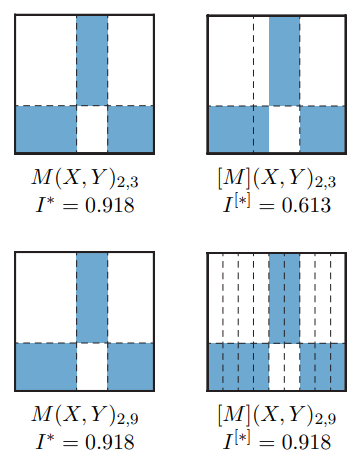
\includegraphics[scale=0.6]{figuras/figure_1_reshef_2016.png}
            \caption{Un esquema que ilustra la diferencia entre la matriz caracter\'istica $M$ y la matriz equicaracter\'istica $[M]$. (Arriba) Cuando se restringe a 2 filas y 3 columnas, la matriz caracter\'istica $M$ se calcula a partir de la rejilla \'optima de 2 por 3. En contraste, la matriz equicaracter\'istica $[M]$ a\'un optimiza la partici\'on m\'as peque\~na de tama\~no 2 pero est\'a restringida a tener la partici\'on m\'as grande como una equipartici\'on de tama\~no 3. Esto resulta en una informaci\'on mutua m\'as baja de 0.613. (Abajo) Cuando se permiten 9 columnas en lugar de 3, la rejilla encontrada por la matriz caracter\'istica no cambia, ya que la rejilla con 3 columnas ya era \'optima. Sin embargo, ahora la matriz equicaracter\'istica utiliza una equipartici\'on en columnas de tama\~no 9, cuya resoluci\'on es capaz de capturar completamente la dependencia entre $X$ e $Y$.}
            \label{fig:matriz_equicaracteristica}
        \end{figure}
        
    
        \begin{defn}
            Sea $(X, Y)$ variables aleatorias conjuntamente distribuidas. Definir
            $$
            I^*((X, Y), k,[\ell])=\max _{G \in G(k,[\ell])} I\left(\left.(X, Y)\right|_G\right),
            $$
            donde $G(k,[\ell])$ es el conjunto de rejillas de $k$ por $[\ell]$ cuya partici\'on del eje $y$ es una equipartici\'on de tama\~no $\ell$. Definir $I^*((X, Y),[k], \ell)$ an\'alogamente.
    
            Definir $I^{[]}((X, Y), k, \ell)$ igual a $I^((X, Y), k,[\ell])$ si $k<\ell$ y $I^((X, Y),[k], \ell)$ en caso contrario.
        \end{defn}
    
        Ahora definimos la matriz equicaracter\'istica en t\'erminos de $I^{[*]}$. En la definici\'on a continuaci\'on, continuamos nuestra convenci\'on de usar corchetes para denotar la presencia de equiparticiones.
    
        \begin{defn}
            Sea $(X, Y)$ variables aleatorias conjuntamente distribuidas. La matriz equicaracter\'istica de poblaci\'on de $(X, Y)$, denotada por $[M](X, Y)$, se define por
            $$
            [M](X, Y)_{k, \ell}=\frac{I^{[*]}((X, Y), k, \ell)}{\log \min \{k, \ell\}},
            $$
            para $k, \ell>1$.
        \end{defn}
    
        La frontera de la matriz equicaracter\'istica se puede definir mediante un l\'imite de la misma manera que la matriz caracter\'istica. Luego tenemos el siguiente teorema.
    
        \begin{thm}
            Sea $(X, Y)$ variables aleatorias conjuntamente distribuidas. Entonces $\partial[M]=\partial M$.
        \end{thm}
        \begin{proof}
            Ap\'endice F de Reshef 2016
        \end{proof}
    
        Dado que cada entrada de la matriz equicaracter\'istica est\'a dominada por alguna entrada en su frontera, la equivalencia de $\partial[M]$ y $\partial M$ produce el siguiente corolario como una simple consecuencia.
    
        \begin{cor}
            Sea $(X, Y)$ variables aleatorias conjuntamente distribuidas. Entonces $\sup [M](X, Y)=$ $M I C_*(X, Y)$.
        \end{cor}
    
        \subsection[short]{El estimador $MIC_e$}
    
        Con la matriz equicaracter\'istica definida, podemos ahora definir nuestro nuevo estimador $\mathrm{MIC}_e$ en t\'erminos de la matriz equicaracter\'istica de muestra, de manera an\'aloga a c\'omo definimos MIC con la matriz caracter\'istica de muestra.
    
        \begin{defn}
            Sea $D \subset \mathbb{R}^2$ un conjunto de pares ordenados. La matriz equicaracter\'istica de muestra $\widehat[{M}](D)$ de $D$ se define como
            $$
            \widehat{[{M}]}(D)_{k, \ell}=\frac{I^{[*]}(D, k, \ell)}{\log \min \{k, \ell\}} .
            $$
        \end{defn}
        \begin{defn}
            Sea $D \subset \mathbb{R}^2$ un conjunto de $n$ pares ordenados, y sea $B: \mathbb{Z}^{+} \rightarrow \mathbb{Z}^{+}$. Definimos
            $$
            M I C_{e, B}(D)=\max _{k \ell \leq B(n)} \widehat{[M]}(D)_{k, \ell}.
            $$
        \end{defn}
    
    
        Con la equivalencia establecida entre la frontera de la matriz caracter\'istica y el de la matriz equicaracter\'istica, es f\'acil demostrar que $\mathrm{MIC}e$ es un estimador consistente de $\mathrm{MIC}*$ mediante argumentos similares a los que aplicamos en el caso de MIC. (Ver Ap\'endice G. Reshef (2016)\cite{Reshef2016}) Espec\'ificamente, mostramos el siguiente teorema, un an\'alogo del Teorema 6.
        
        \begin{thm}
            Sea $f: m^{\infty} \rightarrow \mathbb{R}$ uniformemente continua, y suponga que $f \circ r_i \rightarrow f$ puntualmente. Entonces para cada variable aleatoria $(X, Y)$, tenemos:
    
            $$
            \left.\left(f \circ r_{B(n)}\right)(\widehat{M}]\left(D_n\right)\right) \rightarrow f([M](X, Y)),
            $$
    
            en probabilidad donde $D_n$ es una muestra de tama\~no $n$ de la distribuci\'on de $(X, Y)$, siempre que $\omega(1)<B(n) \leq O\left(n^{1-\varepsilon}\right)$ para alg\'un $\varepsilon>0$.
        \end{thm}
        \begin{proof}
            Ap\'endice A. Reshef (2016) \cite{Reshef2016}
        \end{proof}
    
        Al establecer $f([M])=\sup [M]$, obtenemos como corolario la consistencia de $\mathrm{MIC}_e$.
        
        \begin{cor}
            $M I C_{B}$ es un estimador consistente de $M I C_*$ siempre que $\omega(1)<B(n) \leq O\left(n^{1-\varepsilon}\right)$ para alg\'un $\varepsilon>0$.
        \end{cor}
    
        \subsubsection[computando mic e ]{Computando $MIC_e$}
    
        Tanto el $MIC$ como el $MIC_e$ son estimadores consistentes de $MIC_*$. La diferencia entre ellos radica en que, mientras que el $MIC$ actualmente solo se puede calcular de manera eficiente a trav\'es de una aproximaci\'on heur\'istica, el $MIC_e$ se puede calcular de manera exacta y muy eficiente mediante un enfoque similar al utilizado para aproximar $MIC_*$ que involucra la subrutina \textit{OptimizeXAxis}. Ahora repasaremos los detalles de este enfoque.
    
        Recordemos que, dada una partici\'on fija del eje $x$ $Q$ en $\ell$ columnas, un conjunto de $n$ puntos de datos, una partici\'on ''maestra'' del eje $y$ $\Pi$, y un n\'umero $k$, la subrutina \textit{OptimizeXAxis} encuentra, para cada $2 \leq i \leq k$, una partici\'on del eje $y$ $P_i \subset \Pi $de tama\~no como m\'aximo $i$ que maximiza la informaci\'on mutua inducida por la cuadr\'icula $(P_i, Q)$. El algoritmo realiza esto en un tiempo de $O(|\Pi|^2k\ell)$. Para obtener m\'as detalles sobre \textit{OptimizeXAxis}, consulte la Secci\'on 3.5 de Reshef el al. (2016) \cite{Reshef2016} 
    
        En el par de teoremas a continuaci\'on, se muestran dos formas en que \textit{OptimizeXAxis} se puede utilizar para calcular eficientemente el $MIC_e$. 
    
        \begin{thm}
    
            Existe un algoritmo  \textit{EQUICHAR} que, dada una muestra $D$ de tama\~no $n$ y alg\'un $B \in \mathbb{Z}^{+}$, computa la porci\'on $r_{B(n)}(\widehat{[M]}(D))$ de la matriz equicaracteristica poblacional en tiempo $O\left(n^2 B^2\right)$, que es equivalente a $O\left(n^{4-2 \varepsilon}\right)$ para $B(n)=O\left(n^{1-\varepsilon}\right)$ con $\varepsilon>0$.
        \end{thm}
    
        \begin{proof}
            Describimos el algoritmo y simult\'aneamente acotamos su tiempo de ejecuci\'on. Lo hacemos \'unicamente para las entradas $k, \ell$-\'esimas de $\widehat{[M]}(D)$ que satisfacen $k \leq \ell, k \ell \leq B$. Esto es suficiente, ya que por simetr\'ia, calcular el resto de las entradas requeridas como m\'aximo duplica el tiempo de ejecuci\'on.
    
            Para calcular $\widehat{[M]}(D)_{k, \ell}$ con $k \leq \ell$, debemos fijar una partici\'on equitativa en $\ell$ columnas en el eje $\mathrm{x}$ y luego encontrar la partici\'on \'optima del eje $\mathrm{y}$ de tama\~no como m\'aximo $k$. Si configuramos la partici\'on maestra $\Pi$ del algoritmo \textit{OptimizeXAxis} como una partici\'on equitativa en filas de tama\~no $n$, entonces realiza precisamente la optimizaci\'on requerida. Adem\'as, para un $\ell$ fijo, puede llevar a cabo la optimizaci\'on simult\'aneamente para todos los pares ${(2, \ell), \ldots,(B / \ell, \ell)}$ en tiempo $O\left(|\Pi|^2(B / \ell) \ell\right)=O\left(n^2 B\right)$. Para un $\ell$ fijo, este conjunto contiene todos los pares $(k, \ell)$ que satisfacen $k \leq \ell, k \ell \leq B$. Por lo tanto, para calcular todas las entradas requeridas de $\widehat{[M]}(D)$, solo necesitamos aplicar este algoritmo para cada $\ell=2, \ldots, B / 2$. Hacerlo resulta en un tiempo de ejecuci\'on de $O\left(n^2 B^2\right)$.
        \end{proof}
    
        El algoritmo mencionado anteriormente, aunque es de tiempo polin\'omico, no es lo suficientemente eficiente para su uso en la pr\'actica. Sin embargo, una modificaci\'on simple resuelve este problema sin afectar la consistencia de las estimaciones resultantes. La modificaci\'on se basa en el hecho de que OptimizeXAxis puede usar particiones maestras $\Pi$ adem\'as de la partici\'on equitativa de tama\~no $n$ que utilizamos anteriormente. Espec\'ificamente, configurar $\Pi$ en el algoritmo anterior como una partici\'on equitativa en $c k$ "grupos", donde $k$ es el tama\~no de la partici\'on \'optima m\'as grande que se est\'a buscando, acelera significativamente el c\'alculo. Esta modificaci\'on proporciona una estad\'istica ligeramente diferente, pero que tiene todas las propiedades te\'oricas de $\mathrm{MIC}e$, es decir, una estimaci\'on consistente de $\mathrm{MIC}*$ y un c\'alculo exacto eficiente. Estas propiedades se formalizan en el siguiente teorema
    
        \begin{thm}
            Sea $(X, Y)$  un vertor aleatorio bivariado, y sea $D_n$ y sea una muestra de tama\~no $n$ de la distribucion $(X, Y)$. Para cada $c \geq 1$, existe una matriz $\{\widehat{M}\}^c\left(D_n\right)$ tal que:
            \begin{enumerate}
                \item La funci\'on
                $$
                \widetilde{M I C_{e, B}}(\cdot)=\max {k \ell \leq B(n)}\{\widehat{M}\}^c(\cdot){k, \ell},
                $$
                es un estimador concistente de $M I C_*$ dado $\omega(1)<B(n) \leq O\left(n^{1-\varepsilon}\right)$ para alg\'un $\varepsilon>0$.
                2. Existe un algoritmo \textit{EQUICHARCLUMP} para comparar $r_B\left(\{\widehat{M}\}^c\left(D_n\right)\right)$ en tiempo $O\left(n+B^{5 / 2}\right)$, que equivale a $O\left(n+n^{5(1-\varepsilon) / 2}\right)$ cuando $B(n)=O\left(n^{1-\varepsilon}\right)$.
            \end{enumerate}
            \begin{proof}
                Ap\'endice H. Reshef (2016) \cite{Reshef2016}
            \end{proof}
    
            Para un an\'alisis del efecto del par\'ametro $c$ en el teorema anterior en los resultados del algoritmo \textit{EQUICHARCLUMP}, consulte el Ap\'endice H.3 de Reshef el al. (2016) \cite{Reshef2016}. Estableciendo $\varepsilon=0.6$ en el teorema anterior, obtenemos el siguiente corolario.
    
            \begin{cor}
                $ M I C_*$ puede estimarse de manera consistente en tiempo lineal. 
            \end{cor}
    
            Por supuesto, en tama\~nos de muestra peque\~nos, establecer $\varepsilon=0.6$ ser\'ia indeseable. Sin embargo, nuestro el art\'iculo complementario (Reshef et al.,(2015a) \cite{Reshef2015a}) demuestra emp\'iricamente que en tama\~nos de muestra grandes, esta estrategia funciona muy bien en relaciones t\'ipicas.
    
            Cabe destacar que el algoritmo \textit{EQUICHARCLUMP} dado anteriormente es asint\'oticamente m\'as r\'apido incluso que el algoritmo heur\'istico \textit{APPROX-MIC} utilizado para calcular MIC en la pr\'actica, que se ejecuta en tiempo $O\left(B(n)^4\right)$. Como se demostr\'o en el art\'iculo complementario (Reshef et al., 2015a \cite{Reshef2016}), esta diferencia se traduce en una diferencia sustancial en los tiempos de ejecuci\'on para un rendimiento similar en una gama de tama\~nos de muestra realistas, que va desde una aceleraci\'on de 30 veces en $n=500$ hasta m\'as de 350 veces en $n=10,000$.
        \end{thm}
    
        \subsubsection[eligiendoBn]{Eligiendo $B(n)$}\label{eligiendo_Bn}
            
        Recordemos que, como fue propuesto en Reshef el al. (2011) \cite{Reshef2011}, utilizamos funciones de la forma $B(n)=n^\alpha$. Valores grandes de $\alpha$ conducen a un aumento en el error esperado en reg\'imenes de baja se\~nal ($R^2$ bajos) debido tanto a un sesgo positivo en esos reg\'imenes como a un aumento general en la varianza que afecta predominantemente a esos reg\'imenes. Por otro lado, valores peque\~nos de $\alpha$ llevan a un aumento en el error esperado en reg\'imenes de alta se\~nal (R2 altos) al generar un sesgo negativo en esos reg\'imenes y desplazar la varianza del estimador hacia esos reg\'imenes. En otras palabras, valores m\'as bajos de $\alpha$ son m\'as adecuados para detectar se\~nales m\'as d\'ebiles, mientras que valores m\'as altos de $\alpha$ son m\'as adecuados para distinguir entre se\~nales m\'as fuertes. Esto concuerda con los resultados observados en el trabajo complementario (Reshef et al., (2015a) \cite{Reshef2015a} ), que muestran que valores bajos de $\alpha$ hacen que MICe proporcione pruebas de independencia con mejor potencia, mientras que valores altos de $\alpha$ hacen que MICe tenga una mejor equidad.
    
    
        \subsection[TIC]{\textit{Total Information coefficient ($TIC$)}}
    
        Hasta ahora hemos presentado resultados sobre estimadores del coeficiente de informaci\'on maximal de la poblaci\'on, una cantidad para la cual la equitabilidad es la principal motivaci\'on. Ahora introducimos y analizamos una nueva medida de dependencia, el coeficiente de informaci\'on total ($TIC$). A diferencia del coeficiente de informaci\'on maxima($MIC$), el coeficiente de informaci\'on total no est\'a dise\~nado para la equitabilidad, sino m\'as bien como una estad\'istica de prueba para probar una hip\'otesis nula de independencia.
    
        Comenzamos dando alguna intuici\'on. Recordemos que el coeficiente de informaci\'on maximal es el supremo de la matriz caracter\'istica. Si bien estimar el supremo de esta matriz tiene muchas ventajas, esta estimaci\'on implica tomar un m\'aximo sobre muchas estimaciones de las entradas individuales de la matriz caracter\'istica. Dado que los m\'aximos de conjuntos de variables aleatorias tienden a aumentar a medida que crece el n\'umero de variables, se puede imaginar que este procedimiento puede llevar a un sesgo positivo indeseable en el caso de la independencia estad\'istica, cuando la matriz caracter\'istica de la poblaci\'on es igual a 0. Esto podr\'ia ser perjudicial para las pruebas de independencia, donde la distribuci\'on muestral de una estad\'istica bajo una hip\'otesis nula de independencia es crucial.
        
        La intuici\'on detr\'as del coeficiente de informaci\'on total es que si en cambio consideramos una propiedad m\'as estable, como la suma de las entradas en la matriz caracter\'istica, podr\'iamos esperar obtener una estad\'istica con un sesgo m\'as peque\~no en el caso de independencia y, por lo tanto, una mejor potencia. En resumen, si nuestro \'unico objetivo es distinguir cualquier dependencia de ruido completo, entonces ignorar toda la matriz caracter\'istica de la muestra, excepto su valor m\'aximo, puede descartar una se\~nal \'util, y el coeficiente de informaci\'on total evita esto al sumar todas las entradas.
        
        Cabe destacar que en Reshef et al. (2011)\cite{Reshef2011} se sugiere que otras propiedades de la matriz caracter\'istica pueden permitirnos medir otros aspectos de una relaci\'on dada adem\'as de su fuerza, y se definieron varias de estas propiedades. El coeficiente de informaci\'on total encaja dentro de este marco conceptual. En la siguiente secci\'on definimos el coeficiente de informaci\'on total en el caso de la matriz caracter\'istica ($TIC$) y la matriz equicaracter\'istica ($TIC_e$). Luego demostramos que tanto TIC como TICe producen pruebas de independencia que son consistentes frente a todas las alternativas dependientes. (Al igual que en el caso de $MIC$ y $MIC_e$, $TIC_e$ es m\'as f\'acil de calcular que $TIC$). Finalmente, revisaremos un estudio de simulaci\'on sobre la potencia de las pruebas de independencia basadas en TICe realizado en el paper de Reshef (2016)\cite{Reshef2016} en un conjunto de relaciones elegidas en Simon y Tibshirani (2012)\cite[]{SimonTibshirani}, mostrando que $TIC_e$ supera a otras medidas comunes de dependencia en muchas de las relaciones y se ajusta estrechamente a su rendimiento en el resto.
    
    
        \subsection[definicionyconcitenciatic]{Definici\'on y Consistenc/'ia de TIC}
    
        Comenzamos definiendo dos versiones del coeficiente. En la siguiente definici\'on notemos qu\'e $\widehat{M}$ denota la matriz caracteristica poblacional y $\widehat{[M]}$ denota la matriz equicaracteristica de poblacional.
    
        \begin{defn}
            Sea $D \subset \mathbb{R}^2$ un conjunto de $n$ pares ordenados, y sea $B: \mathbb{Z}^{+} \rightarrow \mathbb{Z}^{+}$. Definimos:
            $$
            T I C_B(D)=\sum_{k \ell \leq B(n)} \widehat{M}(D)_{k, \ell},
            $$
            y
            $$
            T I C_{e, B}(D)=\sum_{k \ell \leq B(n)} \widehat{[M]}(D)_{k, \ell}.
            $$
        \end{defn}
    
        Ahora nos interesa mostrar que estos estad\'isticos nos entregan test de independencia concistente, para esto debemos detenernos y analizar el comportamiento de las cantidades poblacionales an\'alogas. 
    
        \begin{defn}
            Para una matriz $A$	y un n\'umero positivo $B$, la $B$-parcial suma de 	$A$, denotada por  $S_B(A)$, es:
            $$
            S_B(A)=\sum_{k \ell \leq B} A_{k, \ell}.
            $$
            
            Cuando $A$ es una matriz (equi)caracteristica, $S_B(A)$ es la suma sobre todas las entradas correpondientes a mallas con al menos $B$ celdas totales. Por tanto, si $\widehat{M}(D)$ es una matriz equicaracteristica poblacional de $D, S_B(\widehat{M}(D))=\mathrm{TIC}_B(D)$, y lo mismo se mantiene cierto para $S_B(\widehat{[M]}(D))$ and $\mathrm{TIC}_{e, B}(D)$.
            
            Es claro que si $X$ e $Y$ son variables aleatorias estad\'isticamente independientes, se tiene que ambas matrices caracteristicas $M(X, Y)$ y la matriz equicaracteristica $[M](X, Y)$ son identicamente 0 , tal que $S_B(M(X, Y))=S_B([M](X, Y))=0$ para todo $B$. Sin embargo, tambi\'en nos interesa como estas cantidades se comportan cuando las variables $X$ e $Y$ son dependietes. Las siguientes proposiciones nos ayudan a entender esto. La primera nos muestra una cota inferior para los valores de las entradas de ambas $M(X, Y)$ y $[M](X, Y)$. La segunda nos muestra una caracterizaci\'on asint\'otica de como crecen $S_B(M)$ y $S_B([M])$ como funciones de $B$. Estas dos proposiciones son el coraz\'on t\'ecnico de por qu\'e el coeficiente de informaci\'on total produce un test de independencia consistente.
            
            \begin{prop}
                Sea $(X, Y)$ un vector aleatorio bivariado. Si $X$ e $Y$ son estad\'isticamente independientes, entonces $M(X, Y) \equiv[M](X, Y) \equiv 0$. Si no, existe alg\'un $a>0$ y alg\'un entero $\ell_0 \geq 2$ tal que:
                
                $$
                M(X, Y)_{k, \ell,}[M](X, Y)_{k, \ell} \geq \frac{a}{\log \min \{k, \ell\}},
                $$
                ya sea para todo $k \geq \ell \geq \ell_0$, o para todo $\ell \geq k \geq \ell_0$.
            \end{prop}
            \begin{proof}
                Ap\'endice K.1. Reshef (2016) \cite{Reshef2016}
            \end{proof}
            \begin{prop}
                Sean $(X, Y)$ un vector aleatorio bivariado. Si $X$ e $Y$ independites, se tiene que  $S_B(M(X, Y))=S_B([M](X, Y))=0$ para todo $B>0$. Si no, tenemos que $S_B(M(X, Y))$ y $S_B([M](X, Y))$ son ambos $\Omega(B \log \log B)$.
            \end{prop}
            \begin{proof}
                Ap\'endice K.2. Reshef (2016) \cite{Reshef2016}
            \end{proof}
    
            Con las proposiciones presentadas, y siguiendo la misma l\'ogica de los argumentos de convergencia presentados anteriormente, podemos mostrar el resultado principal de esta secci\'on, que las estad\'isticas $TIC$ y $TIC_e$ producen tests de independencia consistentes.
    
            \begin{thm}
                Los estadisticos $T I C_B$ y $T I C_{e, B}$ proporcionan pruebas coherentes de cola derecha de independencia, siempre que $\omega(1)<B(n) \leq O\left(n^{1-\varepsilon}\right)$ para alg\'un $\varepsilon>0$.
            \end{thm}
            \begin{proof}
                Ap\'endice K.3. Reshef (2016) \cite{Reshef2016}
            \end{proof}
    
            En la pr\'actica, usualemente se utiliza el algoritmo  EQUICHARCLUMP \cite[Secci\'on 4.3]{Reshef2016} para computar la matriz equicaracter\'istica, de donde calculamos $\mathrm{TIC}_e$. Este algoritmo no computa la matriz equicaracteristica exactamente. Pero, como es el caso con $\mathrm{MIC}_e$, el uso del algoritmo no afecta las propiedades te\'oricas de la estad\'istica. Esta demostraci\'on se puede encontrar en Reshef el al. (2016) \cite[Ap\'endice H]{Reshef2016}
        \end{defn}
    
        \subsubsection[poder de independencia basado en TICe]{Prueba de Poder de independencia basadas en $TIC_e$}
    
        Ya sabemos que ambos, $TIC$ y $TIC_e$, son consitentes, ahora nos interesa realizar una evaluci\'on emp\'irica de la prueba de poder de independencia basado en $TIC_e$	siendo computado usando al algoritmo \textit{EQUICHARCLUMP}.
    
        En Reshef el at. (2016)\cite{Reshef2016}, para evaluar el poder que tiene esta prueba, se realiza el analisis utilizado por Simon y Tibshirani (2012) \cite{SimonTibshirani}. Este corresponde a un conjunto de relaciones definido por:
    
        $$
        \mathcal{Q}=\left\{\left(X, f(X)+\varepsilon^{\prime}\right): X \sim \text { Unif, } f \in F, \varepsilon^{\prime} \sim \mathcal{N}\left(0, \sigma^2\right), \sigma \in \mathbb{R}_{\geq 0}\right\},
        $$
        
        donde $F$ es el conjunto de relaciones definido en Simon y Tibshirani (2012) \cite{SimonTibshirani}. Estas corresponden a relacion: Lineal, Cuadr\'atica, C\'ubica, Seno (Perido $\frac{1}{8}$), Seno (Periodo $\frac{1}{2}$), $X^\frac{1}{4}$, Circular (tratado como dos semicirculos), y Funci\'on escalera. Detalles de la m\'etodolog\'ia que fue utilizada pueden ser encontrados en la secc\'on 5.2 de Reshef el at. (2016)\cite{Reshef2016}.
    
    
        Los resultados del an\'alisis se presentan en la Figura \ref{reshef_2016_f5}. En primer lugar, la figura muestra que TICe se compara de manera bastante favorable con la correlaci\'on de distancia, un m\'etodo considerado tener un alto poder (Simon y Tibshirani, (2012)\cite{SimonTibshirani}). Espec\'ificamente, $TIC_e$ supera de manera uniforme a la correlaci\'on de distancia en 5 de los 8 tipos de relaciones examinados y se desempe\~na de manera comparable en los otros tres tipos de relaciones. Cabe destacar que la correlaci\'on de distancia tiene muchas ventajas sobre $TIC_e$, incluyendo el hecho de que se generaliza f\'acilmente a relaciones de mayor dimensionalidad y viene con un marco te\'orico elegante y completo.
    
        El an\'alisis tambi\'en muestra que TICe supera en gran medida al coeficiente de informaci\'on maximal ($MIC$) original, y tambi\'en supera a $MIC_e$, respaldando la intuici\'on de que la suma realizada por el primero puede, de hecho, conducir a ganancias sustanciales en poder contra la independencia en comparaci\'on con la maximizaci\'on realizada por el \'ultimo. 
    
    
        \begin{figure}[H] 
            \centering
            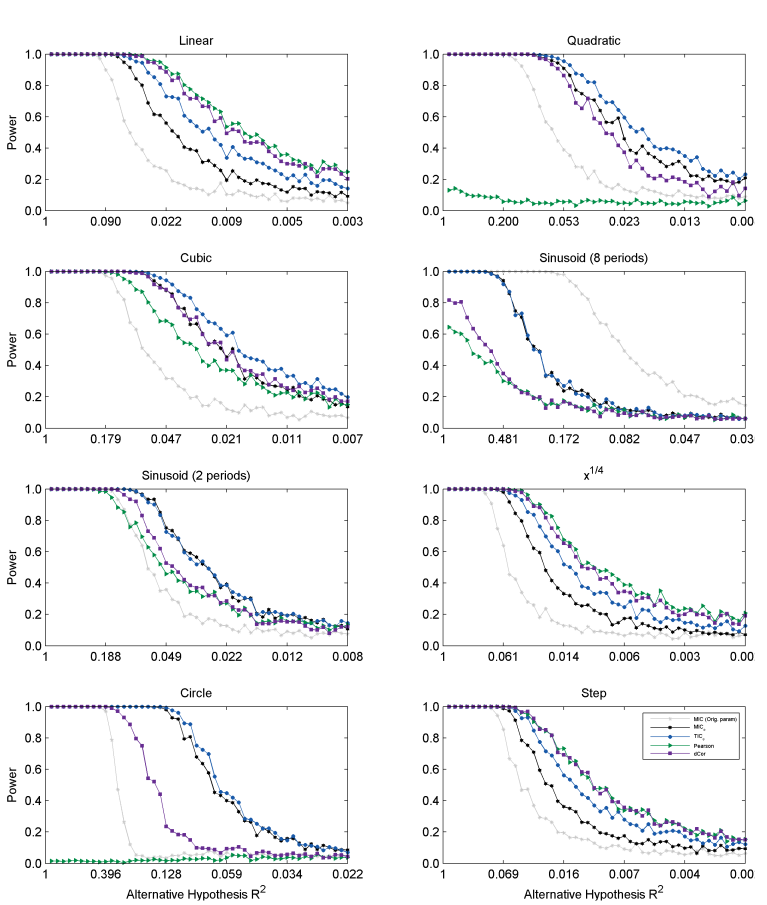
\includegraphics[scale = 0.4]{reshef_2016_fig5.png}
            \caption{Comparaci\'on del poder de prueba de independencia basado en $TIC_e$ (azul) con $MIC$ con par\'ametros predeterminados (gris), $MIC_e$ con los mismos par\'ametros que $TIC_e$ (negro), correlaci\'on de distancia (p\'urpura) y el coeficiente de correlaci\'on de Pearson (verde) en varios tipos de relaciones de hip\'otesis alternativas elegidos por Simon y Tibshirani (2012 \cite{SimonTibshirani}).}
            \label{reshef_2016_f5}
        \end{figure}
    
    
    
        \newpage
    
    
        \subsubsection{Ejemplos}
        Ahora, con una definici\'on clara de como calcular los coeficientes, podemos procesder a un ejemplo de su uso. Para esto usaremos "The Datasaurus Dozon", un conjutno de datos propuesto por Justin Matejka y George Fitzmaurice (2017) \cite{datasaurus}. Este conjunto de datos nos presenta con 13 realciones, visibles en la Figura \ref{datasaurus_fig}, las cuales todas poseen los mismos valores para estad\'isticos descriptivos comunos (Promedio Marginal, Desviac\'on Estandar Marginal, y Correlaci\'on de Pearson), pero son claramente visualmente distinos.
    
        \begin{figure}[H] 
            \centering
            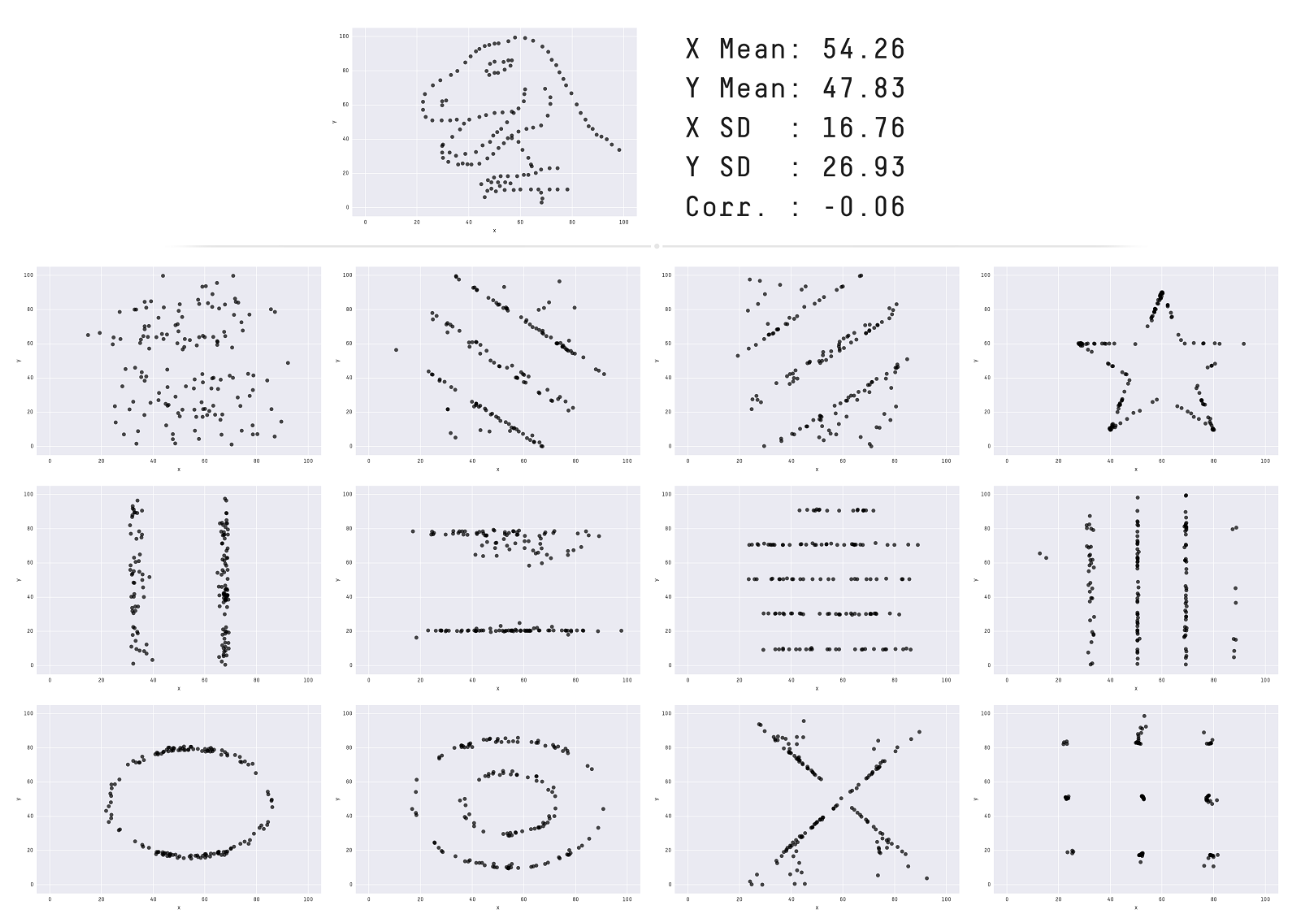
\includegraphics[scale = 0.2]{datasaurusdozon.png}
            \caption{The Datasaurus Dozon", a pesar de compartir los mismos estad\'isticos descriptivos, son visualmente distintos.}
            \label{datasaurus_fig}
        \end{figure}
    
        De particular interes para nosotros es el valor de la correlaci\'on de Pearson de, esta es b\'asicamente cero, lo que nos "deber\'ia" indicar que las relaciones son independientes. Sin embargo, como podemos ver en la Figura \ref{datasaurus_fig}, esto no es cierto. Es por esto que estos datos nos son de gran ayuda. 
    
        Para este ejemplo, tomamos los vectores marginales de cada una de las relaciones, y los colocamos todos en un solo conjunto de datos. Luego de esto utilizamos $TIC_e$ para encontrar los pares que sean m\'as independientes, y finalmente usamos $MIC_e$ para cuantificar la relacion entre estos pares. Los resultados de este analisis se pueden ver en la Figura %\ref{datasaurus_fig2}.
    
        \todo{Rehacer Figura y terminar secci\'on}
    
        \subsubsection[]{Ejemplos}
        \begin{figure}[H]
            \centering
            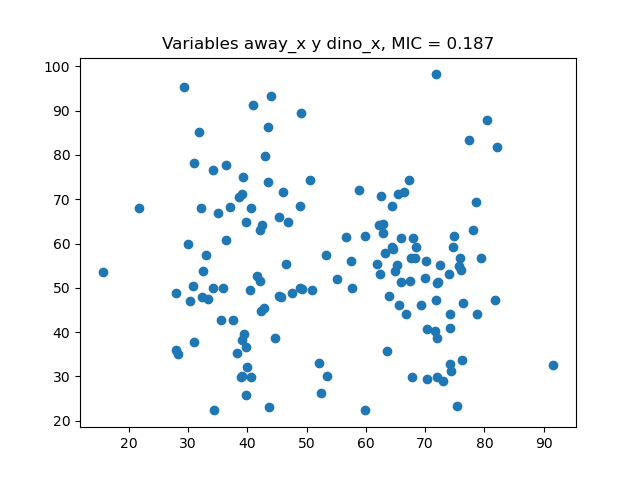
\includegraphics[scale=0.6]{away_x_dino_x_.png}
            \caption{ MIC = 0.187}
            \end{figure}
            
            \begin{figure}[H]
            \centering
            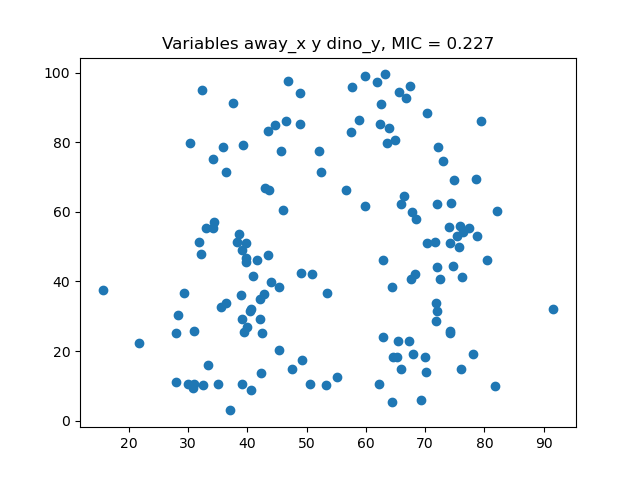
\includegraphics[scale=0.6]{away_x_dino_y_.png}
            \caption{ MIC = 0.227}
            \end{figure}
            
            \begin{figure}[H]
            \centering
            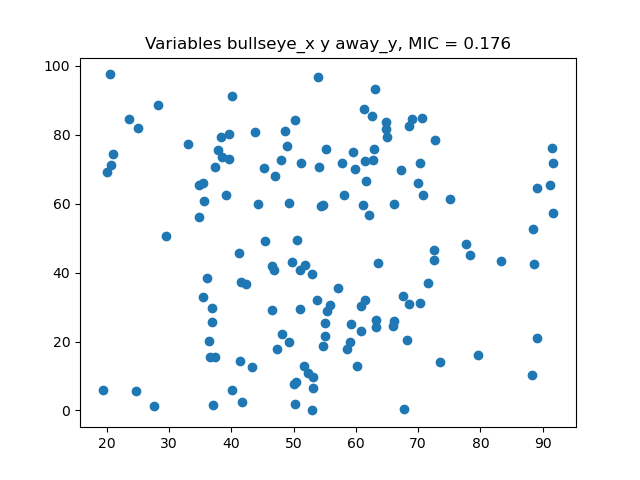
\includegraphics[scale=0.6]{bullseye_x_away_y_.png}
            \caption{ MIC = 0.176}
            \end{figure}
            
            \begin{figure}[H]
            \centering
            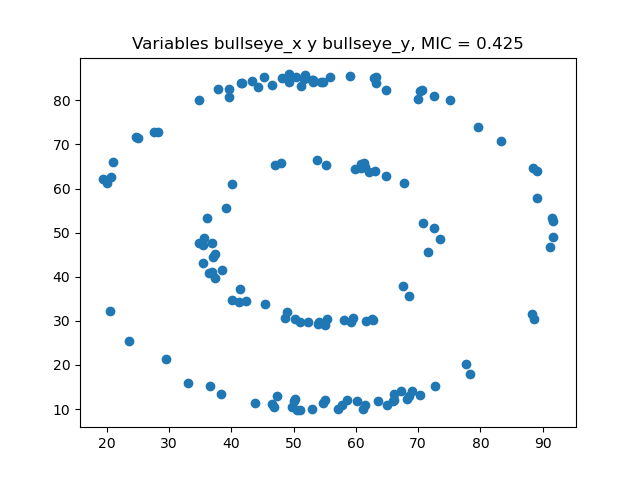
\includegraphics[scale=0.6]{bullseye_x_bullseye_y_.png}
            \caption{ MIC = 0.425}
            \end{figure}
            
            \begin{figure}[H]
            \centering
            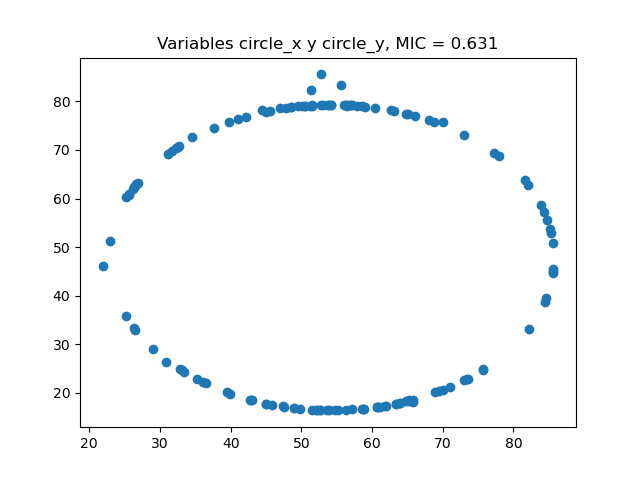
\includegraphics[scale=0.6]{circle_x_circle_y_.png}
            \caption{ MIC = 0.631}
            \end{figure}
            
            \begin{figure}[H]
            \centering
            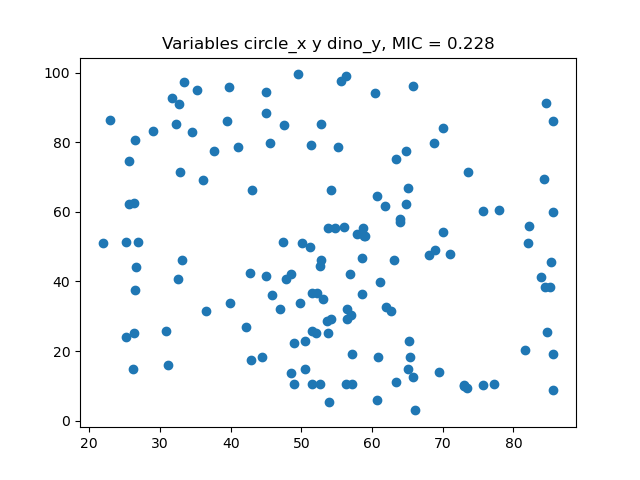
\includegraphics[scale=0.6]{circle_x_dino_y_.png}
            \caption{ MIC = 0.228}
            \end{figure}
            
            \begin{figure}[H]
            \centering
            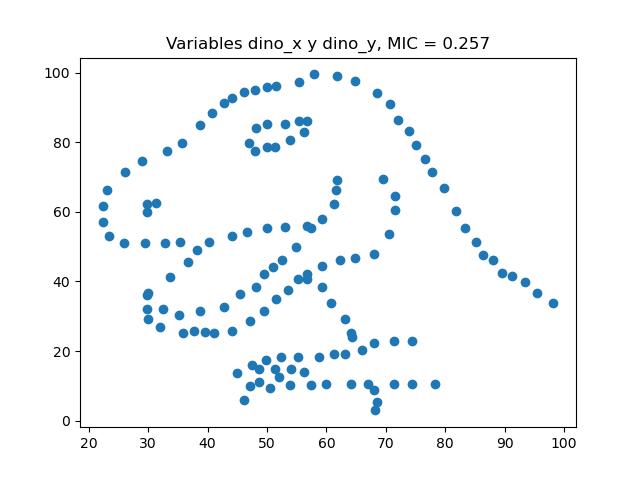
\includegraphics[scale=0.6]{dino_x_dino_y_.png}
            \caption{ MIC = 0.257}
            \end{figure}
            
            \begin{figure}[H]
            \centering
            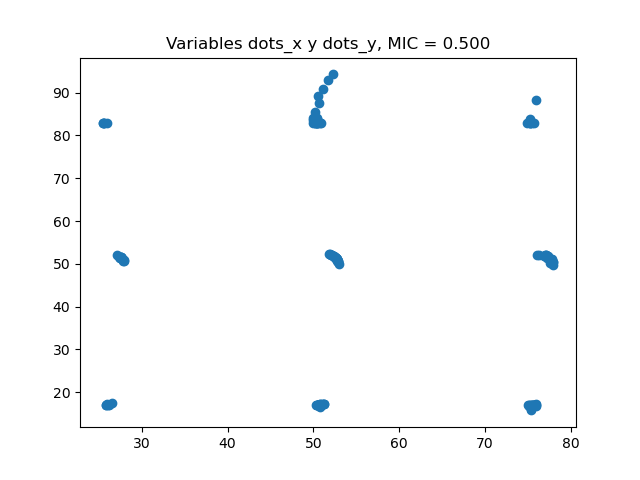
\includegraphics[scale=0.6]{dots_x_dots_y_.png}
            \caption{ MIC = 0.500}
            \end{figure}
            
            \begin{figure}[H]
            \centering
            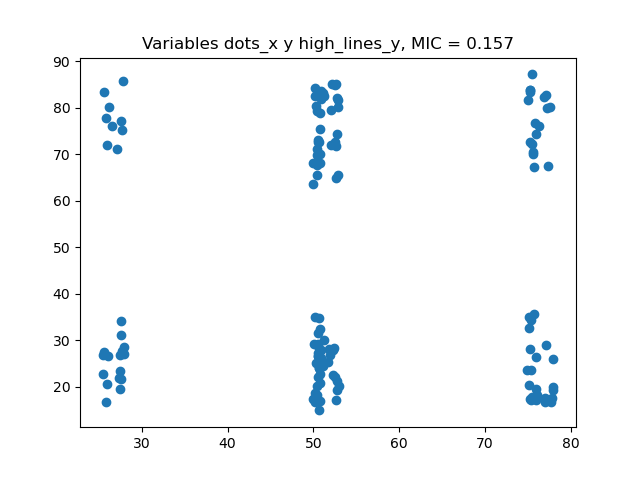
\includegraphics[scale=0.6]{dots_x_high_lines_y_.png}
            \caption{ MIC = 0.157}
            \end{figure}
            
            \begin{figure}[H]
            \centering
            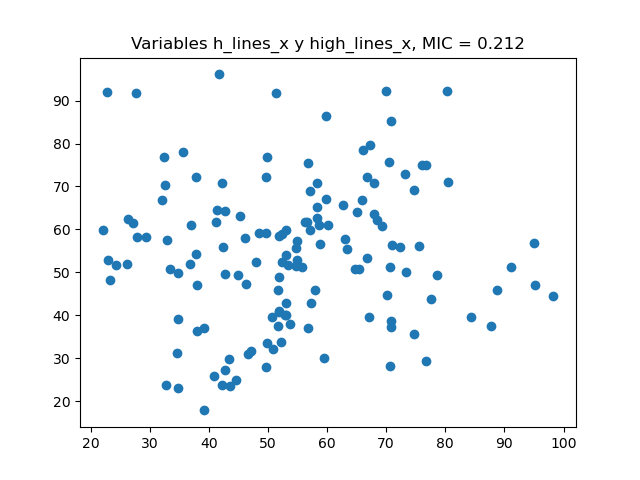
\includegraphics[scale=0.6]{h_lines_x_high_lines_x_.png}
            \caption{ MIC = 0.212}
            \end{figure}
    
            
        % ---------------------------------------------------------------------------------------
\section[Covarianza y Correlaci\'on por Distancia]{Covarianza y Correlaci\'on por Distancia} \label{chap3}

\subsection{Introducci\'on}

En la secci\'on anterior, discutimos el MIC y el TIC, dos medidas de asociaci\'on utilizadas para cuantificar relaciones no lineales entre datos, pero no es la \'unica, y de hecho es cr\'iticada por tener algunas falencias al momento de detectar la fuerza entre relaciones \cite{SimonTibshirani}. Por esto tambi\'en buscamos otra medida que nos ayudar\'a a complementar el an\'alisis de asociaci\'on entre variables, y por esto en este cap\'itulo estudiaremos la Covarianza y Correlaci\'on por Distancia.

La Covarianza por Distancia (cCor) y la Correlaci\'on por distancia (dCor) fueron propuestas por Sz\'ekely, Rizzo, y Bakirov en su trabajo \textit{''Measuring and testing independence by correlation of distances''} (2007) \cite{Szekely2007}, posteriormente tambi\'en propusieton la Covarianza por Distancia Browniana en su trabajo \textit{''Brownian Distance Covariance''} (2009) \cite{Szekely2009}, en donde tambi\'en se demostr\'o que esta coincide con la Covarianza por Distancia tradicional.

Estas son medidas de asociaci\'on no param\'etricas que buscan encontrar relaciones no lineales entre dos conjuntos de datos, en particular establecer una forma de caracterizar independenc\'ia entre dos distribuci\'ones. Dado esto es importante recalcar que, para distribuci\'on de primer momento fin\'ito, la Correlaci\'on por distancia ($\mathcal{R}$) generaliza la idea de correalci\'on en dos formas:

\begin{enumerate}
	\item $\mathcal{R}(X,Y)$ est\'a definido para $X,Y$ de dimensi\'on aleatoria.
	\item $\mathcal{R}(X,Y) = 0$ caracteriza la independenc\'a de $X$ e $Y$.	 
\end{enumerate}

La primera de estas afirmaciones es importante, ya que nos permite utulizar esta medida para comparar im\'agenes sin mayor problema, de todas formas en la secci\'on \ref{chap5} estudiaremos como adaptar est\'as medidas para im\'agnes. En esta secci\'on definiremos estos 3 coeficientes, la relaci\'on entre ellos y verificaremos la afirmaciones realizadas m\'as arriba, para esto comenzaremos con las definiciones. 

\subsection{Definiciones}

Sean $X$ en $\R^p$ y $Y$ en $\R^q$ vectores aleatorios, donde $p$ y $q$ son enteros positivos. Las funciones en min\'uscula $f_X$ y $f_Y$ se utilizarán para denotar las funciones caracter\'isticas de $X$ y $Y$, respectivamente, y su funci\'on caracter\'istica conjunta se denota como $f_{X, Y}$. 

\begin{defn}[Covarianza por distancia]
	La Covarianza por distancia (dCov) entre los vectores aleatorios $X$ e $Y$ con primeros momentos finitos es el n\'umero no negativo $\mathcal{V}(X, Y)$ definido por:
	\begin{equation}
		\begin{aligned}\label{dcov_formula}
			\mathcal{V}^2(X, Y) & =\left\|f_{X, Y}(t, s)-f_X(t) f_Y(s)\right\|^2 \\
			& =\frac{1}{c_p c_q} \int_{\R^{p+q}} \frac{\left|f_{X, Y}(t, s)-f_X(t) f_Y(s)\right|^2}{|t|_p^{1+p}|s|_q^{1+q}} d t d s .
			\end{aligned}
	\end{equation}

	\end{defn}

	Similarmente, la Varianza por distancia (dVar) se define como la raiz cuadrada:

	$$
	\mathcal{V}^2(X)=\mathcal{V}^2(X, X)=\left\|f_{X, X}(t, s)-f_X(t) f_X(s)\right\|^2 .
	$$

	Por definici\'on de la norma $\|\cdot\|$, es claro que  $\mathcal{V}(X, Y) \geq 0$ y $\mathcal{V}(X, Y)=0$ si y solo si $X$ e $Y$ son indepentes.

	\begin{defn} [Correlaci\'on por distancia]
		La correlaci\'on por distancia (dCor) entre los vectores aleatorios $X$ e $Y$ con primer momento finito es el n\'unero no negtivo $\mathcal{R}(X, Y)$ definido por:
		$$
		\mathcal{R}^2(X, Y)= \begin{cases}\frac{\mathcal{V}^2(X, Y)}{\sqrt{\mathcal{V}^2(X) \mathcal{V}^2(Y)}}, & \mathcal{V}^2(X) \mathcal{V}^2(Y)>0 \\ 0, & \mathcal{V}^2(X) \mathcal{V}^2(Y)=0\end{cases}.
		$$

	Algunas propiedades de $\mathcal{R}$ an\'alogo a $\rho$ ser\'an revisadas m\'as adelante. 
	\end{defn}

	Ahora, para el caso muestral, definimos los estad\'isticos de distancia de la siguiente forma. Para una muestra aleatoria $(\mathbf{X}, \mathbf{Y})=\left\{\left(X_k, Y_k\right): k=1, \ldots, n\right\}$ de $n$ ventores aleatorios $(X, Y)$ i.i.d., calculamos las matrices de distancia euclideana  $\left(a_{k l}\right)=\left(\left|X_k-X_l\right|_p\right)$ y $\left(b_{k l}\right)=\left(\left|Y_k-Y_l\right|_q\right)$. Definimos:

	$$
	A_{k l}=a_{k l}-\bar{a}_{k .}-\bar{a}_{. l}+\bar{a}_{. .}, \quad k, l=1, \ldots, n,
	$$
	donde
	$$
	\bar{a}_{k .}=\frac{1}{n} \sum_{l=1}^n a_{k l}, \quad \bar{a}_{. l},=\frac{1}{n} \sum_{k=1}^n a_{k l}, \quad \bar{a}_{. .}=\frac{1}{n^2} \sum_{k, l=1}^n a_{k l} .
	$$
	
	De forma similar, definimos $B_{k l}=b_{k l}-\bar{b}_{k .}-\bar{b}_{\cdot l}+\bar{b}_{. .}$, para $k, l=1, \ldots, n$.

	\begin{defn}[Covarianza y Correlaci\'on por distancia muestral]
		La no negativa Covarianza por distancia muestral $\mathcal{V}_n(\mathbf{X}, \mathbf{Y})$ y la Correlaci\'on por distancia muestral $\mathcal{R}_n(\mathbf{X}, \mathbf{Y})$ estan definidas por
		$$
		\mathcal{V}_n^2(\mathbf{X}, \mathbf{Y})=\frac{1}{n^2} \sum_{k, l=1}^n A_{k l} B_{k l},
		$$
		y
		$$
		\mathcal{R}_n^2(\mathbf{X}, \mathbf{Y})= \begin{cases}\frac{\mathcal{V}_n^2(\mathbf{X}, \mathbf{Y})}{\sqrt{\mathcal{V}_n^2(\mathbf{X}) \mathcal{V}_n^2(\mathbf{Y})}}, & \mathcal{V}_n^2(\mathbf{X}) \mathcal{V}_n^2(\mathbf{Y})>0 \\ 0, & \mathcal{V}_n^2(\mathbf{X}) \mathcal{V}_n^2(\mathbf{Y})=0\end{cases},
		$$
		respectivamente. Adem\'as la Varianza por distancia muestral $\mathcal{V}_n(\mathbf{X})$ est\'a definida por
		$$
		\mathcal{V}_n^2(\mathbf{X})=\mathcal{V}_n^2(\mathbf{X}, \mathbf{X})=\frac{1}{n^2} \sum_{k, l=1}^n A_{k l}^2 .
		$$
	\end{defn}

	Por ultimo, plantearemos los siguientes teoremas que nos entregan  propiedades importantes de la Correlaci\'on por distancia:

	\begin{thm}
		Si $(\mathbf{X}, \mathbf{Y})$ es una muestra aleatoria del vector aleatorio $(X, Y)$, entonces
		$$
		\mathcal{V}n^2(\mathbf{X}, \mathbf{Y})=\left\|f{X, Y}^n(t, s)-f_X^n(t) f_Y^n(s)\right\|^2 .
		$$
	\end{thm}
	\begin{thm}
		Si $E|X|_p<\infty$ and $E|Y|_q<\infty$, entonces casi seguramente
		$$
		\lim _{n \rightarrow \infty} \mathcal{V}_n(\mathbf{X}, \mathbf{Y})=\mathcal{V}(X, Y) .
		$$
	\end{thm}
	
	\begin{cor}
		If $E\left(|X|_p+|Y|_q\right)<\infty$, then almost surely
		$$
		\lim _{n \rightarrow \infty} \mathcal{R}_n^2(\mathbf{X}, \mathbf{Y})=\mathcal{R}^2(X, Y) \text {. }
		$$
	\end{cor}
	\begin{thm}\label{thm3_brcov}
		Para vectores aleatorios $X \in \mathbb{R}^p$ y $Y \in \mathbb{R}^q$ tal que $E\left(|X|_p+\right.$ $\left.|Y|_q\right)<\infty$, se tienen las siguientes propiedades:
		\begin{enumerate}
			\item $0 \leq \mathcal{R}(X, Y) \leq 1$, y $\mathcal{R}=0$ si y solo si $X$ e $Y$ son independientes.
			\item $\mathcal{V}\left(a_1+b_1 C_1 X, a_2+b_2 C_2 Y\right)=\sqrt{\left|b_1 b_2\right|} \mathcal{V}(X, Y)$, para todos los vectores constantes $a_1 \in \mathbb{R}^p, a_2 \in \mathbb{R}^q$, escalares $b_1, b_2$ y matrices ortogonales $C_1, C_2$ en $\mathbb{R}^p$ y $\mathbb{R}^q$, respectivamente.	
			\item Si el vector aleatorio $\left(X_1, Y_1\right)$ es ind. del vector aleatorio $\left(X_2, Y_2\right)$, se tiene
			 $$
			\mathcal{V}\left(X_1+X_2, Y_1+Y_2\right) \leq \mathcal{V}\left(X_1, Y_1\right)+\mathcal{V}\left(X_2, Y_2\right) .
			$$
			La igualdad se cumple si y solo si $X_1$ e $Y_1$ son constantes, o $X_2$ e $Y_2$ son constantes, o $X_1, X_2, Y_1, Y_2$ son mutuamente independientes.

			\item $\mathcal{V}(X)=0$ implica que $X=E[X]$, casi seguramente.
			\item $\mathcal{V}(a+b C X)=|b| \mathcal{V}(X)$, para todos los vectores constantes $a$ en $\mathbb{R}^p$, escalares $b$, y matrices ortogonales $p \times p$ $C$.
			\item Si $X$ e $Y$ son independientes, entonces $\mathcal{V}(X+Y) \leq \mathcal{V}(X)+\mathcal{V}(Y)$. La igualdad se cumple si y solo si uno de los vectores aleatorios $X$ o $Y$ es constante.
		\end{enumerate}
	\end{thm}
	\begin{thm}
	\begin{enumerate}
		\item $\mathcal{V}_n(\mathbf{X}, \mathbf{Y}) \geq 0$.
		\item $\mathcal{V}_n(\mathbf{X})=0$ si y solo si cada observaci\'on de la muestra es id\'entica.
		\item $0 \leq \mathcal{R}_n(\mathbf{X}, \mathbf{Y}) \leq 1$.
		\item $\mathcal{R}_n(\mathbf{X}, \mathbf{Y})=1$ implica que las dimensiones de los subespacios lineales generados por $\mathbf{X}$ y $\mathbf{Y}$ respectivamente son casi seguramente iguales, y si asumimos que estos subespacios son iguales, entonces en este subespacio
		\item $$
		\mathbf{Y}=a+b \mathbf{X} C,
		$$
		para alg\'un vector $a$, n\'umero real no nulo $b$, y matriz ortogonal $C$.
	\end{enumerate}	
	\end{thm}
	demostraci\'ones de todos estos teoremas pueden ser encontrados en Szekely y Rizzo (2009) \cite{Szekely2009}.


	\subsection{Covarianza Browniana}
		
		Para introducir la noci\'on de covarianza browniana, comenzaremos considerando la covarianza cuadrada del producto-momento. Recordemos que una variable prima $X'$ denota una copia independiente e id\'enticamente distribuida (i.i.d.) del símbolo no prima $X$. Para dos variables aleatorias continuas de valores reales, el cuadrado de su covarianza clásica es:

		$$\E[(X-\E(X))(Y-\E(Y))] = \E[(X-\E(X))(X'-\E(X'))(Y-\E(Y))(Y'-\E(Y'))]	$$

		Ahora generalizamos la covarianza al cuadrado y definimos el cuadrado de la covarianza condicional, dadas dos procesos estocásticos de valores reales, $U(\circ)$ y $V(*)$. Obtenemos un resultado interesante cuando U y V son procesos de Wiener independientes.


		Primero, para centrar la variable aleatoria $X$ en la covarianza condicional, necesitamos la siguiente definici\'on. Sea $X$ una variable aleatoria de valores reales y $\{U(t): t \in \R\}$ un proceso estoc\'astico de valores reales, independiente de $X$. La versi\'on centrada de $X$ respecto a $U$ se define por:

		$$
		X_U = U(X)-\int_{-\infty}^{\infty}U(t)dF_X(t)=U(X)-\E[U(X)|U],
		$$

		siempre que la esperanza condicional exista. Notemos que, si $id$ es la identidad, $X_{id}=X-\E[X]$. 

		Ahora, sea $\mathcal{W}$ un movimiento Browniano/Wiener de una dimensi\'on en ambos lados con esperanza cero y funci\'on de covarianza.
		\begin{equation}\label{brw_covariamce}
			|s|+|t|-|s-t|=2\min(s.t)
		\end{equation}
			

		Esto es dos veces la covarianza estandar para un proceso Wiener. Pero en adelante el factor de dos nos simplificar\'a algunos calculos, por lo que en el resto de la secci\'on asumiermos esta funci\'on de covarianza \ref{brw_covariamce} para $\mathcal{W}$. Ya con esto, podemos definir la Covarianza Browniana 

		\begin{defn}[Covarianza Browniana]
			La Covarianza Browniana (o covarianza Wiener) de dos variables aleatorias con valores reales $X$ e $Y$, con segundos monetos fin\'itos es el n\'umero no negativo definido por su cuadrado:
			\begin{equation}\label{brw_cov}
				\mathcal{W}^2(X,Y)={Cov}_{{W}^2}(X,Y)=\E[X_{W}X'_{W}Y_{W'}Y'_{W'}],
			\end{equation}

			donde $({W},{W'})$ no dependen de $(X,X',Y.Y')$.
		\end{defn}

		Tomemos en cuenta que si ${W}$ en ${Cov}_{{W}^2}$ es reemplazada por la funci\'on identidad (no aleatoria) $id$, entonces ${Cov}_{id}(X, Y) = |{Cov}(X, Y)| = |\sigma_{X,Y}|$, el valor absoluto de la covarianza del producto-momento de Pearson. Mientras que la covarianza del producto-momento estandarizada, la correlación de Pearson ($\rho$), mide el grado de relaci\'on lineal entre dos variables con valores reales, veremos que la covarianza estandarizada de Brownian mide el grado de todos los tipos posibles de relaciones entre dos variables aleatorias con valores reales.

		La definición de ${Cov}_{{W}^2}$ se puede extender a procesos aleatorios en dimensiones superiores de la siguiente manera. Si $X$ es una variable aleatoria con valores en $\R^p$ y $U(s)$ es un proceso aleatorio (campo aleatorio) definido para todos los $s \in \R^p$ e independiente de $X$, define la versión centrada en $U$ de $X$ como

		$$
			X_U=\E(X)-\E[U(X)|U]
		$$
		siempre que la expectativa condicional exista.

		\begin{defn}
			Si $X$ es un vector aleatorio con valores en $\R^p$ y $Y$ es un vector aleatorio con valores en $\R^q$, y $U(s)$ y $V(t)$ son procesos aleatorios, definamos para todo $s\in\R^p$, $t\in\R^q$, entonces la covarianza (U,V) de $X$ e $Y$ es el n\'umero no negativo definido por su cuadrado:
			\begin{equation}\label{eq_35_brcov}
				{Cov}^2_{(U,V)}(X,Y) = \E[X_U X'_U Y_V Y'_V],
			\end{equation}
				
			siempre que el lado derecho sea positivo y finito.
		\end{defn}

		En particular, si ${W}$ y ${W'}$ son procesos brownianos con funci\'on de covarianza \ref{brw_covariamce} en $\R^p$ y $\R^q$ respectivamente, la Covarianza Browniana de $X$ e $Y$ esta definida por:

		\begin{equation}
			\mathcal{W}^2(X,Y) = Cov^2_W(X,Y) = Cov^2_{W,W'}(X,Y).
		\end{equation}

		De la misma forma, para variables aleatorias con varianza finita podemos definir la Varianza Browniana:

		\begin{equation}
			\mathcal{W}(X) = Cov_W(X) = Cov_{W}(X,X).
		\end{equation}
		
		Y con esto, podemos definir la correlaci\'on Browniana:
		
		\begin{defn}[Correlaci\'on Browniana]
			Definimos la correalci\'on Browniana de dos variables aleatorias con valores reales $X$ e $Y$ con segundos momentos finitos como:
			\begin{equation}	
				Cor_W(X,Y) = \frac{\mathcal{W}}{\sqrt[]{\mathcal{W}(X)\mathcal{W}(Y)}},
			\end{equation}
			siempre que el denominador no sea 0; otro caso $Cor_W(X,Y) = 0$.
		\end{defn}

		Ahora, solo nos queda probar que $Cov_W(X,Y)$ existe para vectores aleatorios de segundos momentos finitos, y con esto derivar la Covarianza Browniana. Para esto, tenemos el siguiente teorema:

		\begin{thm}\label{thm_exists_cov_browniana}
			Si $X$ es un vector aleatorio con valores en $\R^p$, e $Y$ es un vector aleatorio con valores en $\R^q$, y $\E(|X|^2+|Y|^2)>\infty$, entonces $\E[X_{W}X'_{W}Y_{W'}Y'_{W'}]$ es no negativo y finito, y:
			\begin{align}
				\mathcal{W}^2(X,Y) &= \E[X_{W}X'_{W}Y_{W'}Y'_{W'}]\\
								   &= \E|X-X'||Y-Y'| + \E|X-X'|\E|Y-Y'| - \label{cov_browniana_exists} \\ 
								   &\qquad - \E|X-X'||Y-Y''|\E|X-X''||Y-Y'|,\label{eq_37_brcov}
 			\end{align}
			donde $(X,Y)$, $(X',Y')$, y $(X'',Y'')$ son iid.
		\end{thm}
		\begin{proof}
			Notemos que
			$$
			\begin{aligned}
			E\left[X_W X_W^{\prime} Y_{W^{\prime}} Y_{W^{\prime}}^{\prime}\right] & =E\left[E\left(X_W Y_{W^{\prime}} X_W^{\prime} Y_{W^{\prime}}^{\prime} \mid W, W^{\prime}\right)\right] \\
			& =E\left[E\left(X_W Y_{W^{\prime}} \mid W, W^{\prime}\right) E\left(X_W^{\prime} Y_{W^{\prime}}^{\prime} \mid W, W^{\prime}\right)\right] \\
			& =E\left[E\left(X_W Y_{W^{\prime}} \mid W, W^{\prime}\right)\right]^2,
			\end{aligned}
			$$
			y esto es siempre no negativo. Para finitud, es suficiente demostrar que todos los factores en la definici\'on de  $\operatorname{Cov}_W(X, Y)$ tienen cuartos momentos finitos. La ecuaci\'on \ref{cov_browniana_exists} se basa en la forma especial de la funci\'on de covarianza de \ref{brw_covariamce} de $W$. El resto de la demostraci\'on se puede encontrar en el ap\'endice de /Szehely and Rizzo (2009)\cite{Szekely2009}.	
		\end{proof}

	\subsection{Equivalencia entre covarianzas}
	
	Ahora estudiaremos la equivalencia entre la Covarianza por distancia y la Covarianza Browniana. Pero antes de esto necesitamos plantear el siguiente lema:

	\begin{lem}\label{lemma_1_brcov}
		Si $0<\alpha<2$, entonces para todo $x$ en $\R^d$
		$$
		\int_{\R^d} \frac{1-\cos \langle t, x\rangle}{|t|_d^{d+\alpha}} d t=C(d, \alpha)|x|_d^\alpha,
		$$
		donde
		$$
		C(d, \alpha)=\frac{2 \pi^{d / 2} \Gamma(1-\alpha / 2)}{\alpha 2^\alpha \Gamma((d+\alpha) / 2)},
		$$
		y $\Gamma(\cdot)$ es la funci\'on completea gamma. Las integrales en 0 y $\infty$ se entienden en el sentido de valor principal: $\lim_{\varepsilon \rightarrow 0} \int_{\R^d \backslash\left\{\varepsilon B+\varepsilon^{-1} B^c\right\}}$, donde $B$ es la bola unitaria (centrada en 0) en $\R^d$ y $B^c$ es el complemento de $B$.
	\end{lem}
	Una demostraci\'on de este lemma puede ser entontrada en Székely and Rizzo (2007) \cite{Szekely2007}. El Lemma \ref{lemma_1_brcov}
	sugiere que la funci\'on de pesos
	\begin{equation}\label{eq_23_brcov}
	w(t, s ; \alpha)=\left(\left.\left.C(p, \alpha) C(q, \alpha)|t|_p^{p+\alpha}\right|s\right|_q ^{q+\alpha}\right)^{-1}, \quad 0<\alpha<2 .	
	\end{equation}

	En el caso m\'as simple correspondiente a $\alpha=1$ y norma euclidiana $|x|$,
	\begin{equation}\label{eq_24_brcov}
		w(t, s)=\left(c_p c_q|t|_p^{1+p}|s|_q^{1+q}\right)^{-1},
		\end{equation}
	
	donde,
	\begin{equation}\label{eq_25_brcov}
		c_d=C(d, 1)=\frac{\pi^{(1+d) / 2}}{\Gamma((1+d) / 2)} .
	\end{equation}
	
	(La constante $2 c_d$ es el \'area de la esfera unitaria en $\R^{d+1}$).
	\begin{rem}
		El Lemma \ref{lemma_1_brcov} es aplicado para evaluar el integrando en \ref{dcov_formula} para las funciones de peso \ref{eq_23_brcov} y \ref{eq_24_brcov}. Por ejemplo, si $\alpha=1$ \ref{eq_24_brcov}, entonces por el Lemma \ref{lemma_1_brcov} existen constantes $c_p$ y $c_q$ tal que para $X$ en $\R^p$ y $Y$ en $\R^q$,
		$$
		\begin{gathered}
		\int_{\mathbb{R}^p} \frac{1-\exp \{i\langle t, X\rangle\}}{|t|p^{1+p}} d t=c_p|X|_p, \quad \int{\mathbb{R}^q} \frac{1-\exp \{i\langle s, Y\rangle\}}{|s|_q^{1+q}} d s=c_q|Y|_q, \\
		\int_{\mathbb{R}^p} \int_{\mathbb{R}^q} \frac{1-\exp \{i\langle t, X\rangle+i\langle s, Y\rangle\}}{|t|_p^{1+p}|s|_q^{1+q}} d t d s=c_p c_q|X|_p|Y|_q
		\end{gathered}
		$$
	\end{rem}
	
	Ya con esto, podemos pasar el resultado principal de esta secci\'on, con el siguiente teorema.
	

	\begin{thm}\label{thm_8_brcov}
		Para un $X \in \R^p, Y \in \R^q$ arbitrario, con segundos momentos finitos
			$$
			\mathcal{W}(X, Y)=\mathcal{V}(X, Y) .
			$$
			\end{thm}
	
	\begin{proof}
		
	Proof. Ambos $\mathcal{V}$ y $\mathcal{W}$ son no negativos, por tanto, basta por demostrar que sus cuadrados coinciden. Para esto, primero notemos Lemma \ref{lemma_1_brcov} puede ser aplicado para evaluar $\mathcal{V}^2(X, Y)$. En el numerador de la integral tenemos t\'erminos como:
	
	$$
	E\left[\cos \left\langle X-X^{\prime}, t\right\rangle \cos \left\langle Y-Y^{\prime}, s\right\rangle\right],
	$$

	donde $X, X^{\prime}$ son i.i.d. y $Y, Y^{\prime}$ son i.i.d. Ahora, aplicando la identidad:
	$$
	\cos u \cos v=1-(1-\cos u)-(1-\cos v)+(1-\cos u)(1-\cos v)
	$$
	y el Lemma \ref{lemma_1_brcov} para simplificar el integrando. Despu\'es de cancelar en el numerador del integrando, queda por evaluar integrales del tipo:

	$$
	\begin{aligned}
	& E \int_{\R^{p+q}} \frac{\left.\left[1-\cos \left\langle X-X^{\prime}, t\right\rangle\right]\left[1-\cos \left\langle Y-Y^{\prime}, s\right\rangle\right)\right]}{|t|^{1+p}|s|^{1+q}} d t d s \\
	& \quad=E\left[\int_{\R^p} \frac{1-\cos \left\langle X-X^{\prime}, t\right\rangle}{|t|^{1+p}} d t \times \int_{\R^q} \frac{1-\cos \left\langle Y-Y^{\prime}, s\right\rangle}{|s|^{1+q}} d s\right] \\
	& =c_p c_q E\left|X-X^{\prime}\right| E\left|Y-Y^{\prime}\right|
	\end{aligned}
	$$
	Luego de esto, y simplificando, obtenemos:
	$$
	\begin{aligned}
	\mathcal{V}^2(X, Y)= & E\left|X-X^{\prime}\right|\left|Y-Y^{\prime}\right|+E\left|X-X^{\prime}\right| E\left|Y-Y^{\prime}\right| \\
	& -E\left|X-X^{\prime}\right|\left|Y-Y^{\prime \prime}\right|-E\left|X-X^{\prime \prime}\right|\left|Y-Y^{\prime}\right|,
	\end{aligned}
	$$
	y esta es exactamente igual a la expresi\'on \ref{eq_37_brcov} obtenida para $\mathcal{W}^2(X, Y)$ en el Teorema \ref{thm_exists_cov_browniana}.
	\end{proof}

	Como corolario del Teorema \ref{thm_8_brcov}, tenemos que las propiedades de la Covarianza Browniana para vectores aleatorios $X$ e $Y$ con segundos momentos finitos son las mismas propiedades establecidas para la Covarianza por distancia $\mathcal{V}(X, Y)$ en el Teorema \ref{thm3_brcov}.
	
	El sorpredente resultado de que la Covarianza Browniana es igual a la Covarianza por distancia, exactamente como se define en \ref{dcov_formula} para $X \in \R^p$ e $Y \in \R^q$, es paralelo a un caso especial familiar cuando $p=q=1$. Para bivariados $(X, Y)$ encontramos que $\mathcal{R}(X, Y)$ es un contraparte natural del valor absoluto de la correlaci\'on de Pearson. Es decir, si en \ref{eq_35_brcov} $U$ y $V$ son la funci\'on no aleatoria m\'as simple $id$, entonces obtenemos el cuadrado de la covarianza de Pearson $\sigma_{X, Y}^2$. Luego, si consideramos los procesos aleatorios m\'as fundamentales, $U=W$ y $V=W^{\prime}$, obtenemos el cuadrado de la covarianza por distancia, $\mathcal{V}^2(X, Y)$.

\subsection{Ejemplos}

	\todo{usar datasaurus para mostrar los coeficientes}

	\newpage
\blankpage
% ---------------------------------------------------------------------------------------
\chapter{Otros M\'etodos de Comparaci\'on de Im\'agenes}\label{chap3}


\section{Introducci\'on}

En la secci\'on anterior nos enfocamos en describir con detalle el Coeficiente de Informaci\'on M\'axima (MIC), esta medida de correalci\'on es una de las m\'as poderosas al momento de encontrar relaciones entre varibales, y tambi\'en una de las m\'as complejas, motivo por el cu\'al una secci\'on fue dedicada a esta. A pesar de eso, tenemos otros coeficientes tambi\'en poderosos y que nos ayduar\'an a caracterizar la relaci\'on que existe entre las im\'agenes transformadas y sus primitivas. 

En este cap\'itulo estudiaremos 3 medidas de correalci\'on, las que finalmente usaremos en la compraci\'on de las im\'agenes, estas las podemos separar en dos categorías. La primera, que corresponde a la Correlaci\'on M\'axima Local\cite{Chen2012} y la Correlaci\'on por Distancia \cite{Szekely2009}, estas son dos medidas avanzados que buscan relaciones no lineales entre conjuntos de datos. La segunda categor\'ia corresponde unicamente a la Correlaci\'on de Pearson la cu\'al es la medida m\'as utilizada para comparar dos conjuntos, pero est\'a limitada a solo encontrar relaciones lineales entre los datos.

Definiremos los coeficientes, revisaremos algunas de sus propiedades y finalmente discutiremos la inefectividad del coeficiente de Pearson para comparar im\'agenes. Luego en la secci\'on posterior estdiaremos el concepto de Equitatibilidad y lo usaremos para comparar los coeficientes. 

\section[]{Correlaci\'on M\'axima local} 

	%chen2010.pdf

	\subsection{Introducci\'on}


	La correlaci\'on local, tamb\'ien conodica como coeficiente no param\'etrico de Chen, o coeficiente de Chen, es un coeficiente que busca detectar relaciones no lineales basado en la integral de correlaci\'on. Este fue propuesto por Chen et al. en su trabajo \textit{A Nonparametric Approach to Detect Nonlinear Correlation in Gene Expression} (2012) \cite{Chen2012}. Este coeficiente es una medida de asociaci\'on no param\'etrica que puede detectar relaciones no lineales entre dos variables, esto lo hace a trav\'es de un m\'etodo similar al de aproximaci\'on lineal por secci\'ones. 

	La integral de correlaci\'on examina la distribuci\'on acumulativa de distancias entre puntos en una serie de tiempo, en base a esto y con algunas modificaciones, se puede utilizar para estimar patrones y asociaciones globales. 


	\subsection{Definiciones}

	Defnimamos primero el coraz\'on del coeficiente, la integral de correlaci\'on:

	\begin{defn}[Correlaci\'on Integral]
		Sea $z_1,\dots,z_N$ una serie de tiempo de $N$ observaciones y sea $r\in\R_{>0}$. Definimos la integral de correlaci\'on $I(r)$ una funci\'on indicadora definida como:
		$$
		I(r)=\lim _{N \rightarrow \infty}\left\{\frac{1}{N^{2}} \sum_{i, j=1}^{N} I\left(\left|z_{i}-z_{j}\right|<r\right)\right\}.
		$$
	\end{defn}

	La integral de correlaci\'on cuantifica el el n\'umero promedio de vecinos dentro de un radio $r$. Notemos que esta definici\'on sigue teniendo sentido cuando los datos no son series de tiempo, solo requerimos de una indexaci\'on de los estos.

	Para desarrollar una medida de asociaci\'on entre vectores, $x$ e $y$, modificamos la definici\'on de $I(r)$ como sigue. Sean $z_i=(x_i,y_i)$ con $i=1,\dots, N$ las observaciones en el conjunto de datos. Con esto definimos:

	\begin{defn}[Correlaci\'on Integral entre vectores]
		Sean $x= \{x_1,\dots,x_N\} $ e $y=\{y_1,\dots,y_N\}$ dos vectores de $N$ observaciones y sea $r\in\R_{>0}$. Definimos la integral de correlaci\'on $\hat{I}(r)$ entre $x$ e $y$ como:
		$$\hat{I}(r)=\frac{1}{N^{2}} \sum_{i, j=1}^{N} I\left(\left|\begin{pmatrix}
			x_{i} \\
			y_{i}
		  \end{pmatrix}-\begin{pmatrix}
			x_{j} \\
			y_{j}
		  \end{pmatrix}\right|<r\right)$$,
		donde $|\cdot|$ es la norma euclidiana. En adelante, al referirnos a la Integral de Correlaci\'on nos referiremos a esta definici\'on, a menos que se indique lo contrario.

	\end{defn}
	
	Notemos que las distancias obsevadas son adem\'as linealmente transformadas para que se encuentren entres 0 y 1 antes de calcular $\hat{I}$. Es importante destacar que $\hat{I}$a tiene las propiedades de una funci\'on de distribuci\'on acumulativa. Es no decreciente entre 0 y 1 y continua por la derecha. La funci\'on $\hat{I}(r)$ descrive el patr\'on global de distancias entre vecinos. 

	El inter\'es principal es la definici\'on de una metrica para cuantificar la asosiaci\'on no lineal estudiando patrones locales. Dado esto, definimos la densidad de vecinos $D$ de forma similar a la derivada de $\hat{I}$: 
	\begin{defn} [Densidad de Vecinos]
		Dados $x= \{x_1,\dots,x_N\} $, $y=\{y_1,\dots,y_N\}$ y su respectiva Integral de correalci\'on $\hat{I}(r)$
		$$
		\hat{D}(r)= \frac{\vartriangle\hat{I}(r)}{\vartriangle r},
		$$
		donde $\vartriangle\hat{I}(r)$ denota un cambio en $\hat{I}(r)$ y $\vartriangle r$ la magnitud de este.
	\end{defn}
	
	La densidad de vecinos observada es evaluada en radio distreto r, con $r=0,1/m, 2/m, \dots, 1$, con $m$ es un grosor de malla arbitrario que determina $\vartriangle r = \frac{1}{m}$. Una funci\'on de suavizado autom\'atico usando validaci\'on cruzada es usada para elegir un \'optimo el tama\~no $m$ (Vilela et al. 2007) y se aplica para suavizar $D(r)$. En el paper, el tama\~no predeterminado $m$ se establece como $N$, el n\'umero de observaciones y en este trabajo usaremos el mismo $m$. El estad\'istico $\hat{D}$ es una aproximaci\'on discreta de $d\hat{I}(r)/d r$, la cual tiene las propiedades formales de una probabilidad funci\'on de densidad. Por lo tanto, con un ligero abuso de terminolog\'ia nos referimos a $\widehat{D}(r)$ como una distribuci\'on.

	En base a esto definimos la correlaci\'on local. Intuitivamente, las distancias entre los puntos de datos entre dos variables correlacionadas diferir\'ian de las distancias entre dos variables no correlacionadas. 
	
	\begin{defn}[Correlaci\'on Local]
	
		Sea $\widehat{D_0}(r)$ la estimaci\'on de una distribuci\'on nula, que se compone de dos vectores sin asociaci\'on. Definimos la correlaci\'on local ($\ell(r)$) como la desviaci\'on de D de la de la distribuci\'on nula a una distancia vecina dada r:

		$$
			\ell(r)=\widehat{D}(r)-\widehat{D}_{0}(r),
		$$	

		donde $\widehat{D}(r)$ es la distribuci\'on asociada a los vectores que queremos comparar.

	\end{defn}

	Este enfoque no asume ninguna distribuci\'on param\'etrica. La flexibilidad de este m\'etodo facilita el cambio de la distribuci\'on nula a cualquier distribuci\'on de inter\'es. 
	
	Por ultimo, definimos el coficiente como de correlaci\'on local m\'axima, o coeficiente de Chen como:

	\begin{defn}
		Sea $\ell(r)$ la funci\'on de correlaci\'on local entre dos vectores, definimos el coeficiente de correlaci\'on local m\'axima como:

		$$
		M=\max _{r}\{|\ell(r)|\}
		$$

		con $r\in[0,1]$. Recordemos que las distancias fueron nomralizadas.
		
	\end{defn}
	La interpretaci\'on de $\ell(r)$ como la diferencia de dos distribuciones implica que $M$ puede interpretarse como la distancia bajo la norma del supremo entre $\widehat{D}$ y $\widehat{D_0}$. En otras palabras, definimos el estad\'istico M como la desviaci\'on m\'axima entre dos densidades vecinas subyacentes.

\section[]{\textit{Distance Covariance \& Distance Correlation}} 

\subsection{Introducci\'on}


La Covarianza por Distancia  y la Correlaci\'on por distancia  fueron propuestas por Sz\'ekely, Rizzo, y Bakirov en su trabajo \textit{''Measuring and testing independence by correlation of distances''} (2007) \cite{Szekely2007}, posteriormente tambi\'en propusieton la Covarianza por Distancia Browniana en su trabajo \textit{''Brownian Distance Covariance''} (2009) \cite{Szekely2009}, en donde tambi\'en se demostr\'o que esta coincide con la Covarianza por Distancia tradicional.

De la misma forma que las medidas que hemos visto anteriormente, estas son medidas de asociaci\'on no param\'etricas que buscan encontrar relaciones no lineales entre dos conjuntos de datos, en particular establecer una forma de caracterizar independenc\'ia entre dos distribuci\'ones. Dado esto es importante recalcar que, para distribuci\'on de primer momento fin\'ito, la Correlaci\'on por distancia ($\mathcal{R}$) generaliza la idea de correalci\'on en dos formas:

\begin{enumerate}
	\item $\mathcal{R}(X,Y)$ est\'a definido para $X,Y$ de dimensi\'on aleatoria.
	\item $\mathcal{R}(X,Y) = 0$ caracteriza la independenc\'a de $X$ e $Y$.	 
\end{enumerate}

La primera de estas afirmaciones es importante, ya que nos permite utulizar esta medida para comparar im\'agenes sin mayor problema, de todas formas en la secci\'on \ref{chap5} estudiaremos como adaptar est\'as medidas para im\'agnes. En esta secci\'on definiremos estos 3 coeficientes, la relaci\'on entre ellos y verificaremos la afirmaciones realizadas m\'as arriba, para esto comenzaremos con las definiciones. 

\section[]{Correlaci\'on de Pearson}

	\subsection{Introducci\'on}
	
		donde se publico, como su ocupa, despcion en palabras
	 
	\section{Definiciones}
	
	El coef. se define como:
	\begin{equation}\label{pearson_orig}
		\rho_{X,Y}=\frac{cov(X,Y)}{\sigma_X\sigma_Y}
	\end{equation}
	
	Para una muestra de tama\~no $N$, tenemos:
	
	\begin{equation}\label{pearson_r}
		r=\frac{\sum_{i}^N\left(x_{i}-\bar{x}\right)\left(y_{i}-\bar{y}\right)}{\sqrt{\sum_{i}^n\left(x_{i}-\bar{x}\right)^{2}} \sqrt{\sum_{i}^n\left(y_{i}-\bar{y}\right)^{2}}}
	\end{equation}
	
	Con $x_i,y_i$ elementos de la muestra y $\bar{x},\bar{y}$ sus respectivos promedios.
	
	Hablar de The Ineffectiveness of the Correlation Coefficient for Image Comparisons
	
	\newpage
\blankpage
\chapter{Equitabilidad}\label{chap4}

	\section{Introducci\'on}

	La equitabilidad ha sido descrita de manera informal por Reshef et al. como la capacidad de una estad\'istica para "asignar puntuaciones similares a relaciones igualmente ruidosas de diferentes tipos" \cite{Reshef2011}. Aunque \'util, esta definici\'on informal es imprecisa en el sentido de que no especifica lo que se entiende por "ruidoso" o "similar", y no especifica para qu\'e relaciones debe cumplirse la propiedad mencionada.

	En su trabajo posterior \textit{''Equitability, interval estimation, and statistical power''}, Reshef et al. (2015) \cite{Reshef2015}, se formaliz\'o la idea de Equitabilidad a travez del concepto del intervalo interpretativo, que funciona como estimaci\'on en intervalos de la cantidad de ruido presente en una relaci\'on de tipo desconocida. 

	En el contexto de este trabajo, nos interesa que las medidas de dependencia sean equitativas puesto que esto nos asegura que la medida de dependencia no est\'a sesgada hacia un tipo de relaci\'on en particular, y por lo tanto, nos ser\'a \'util para comprar comparar las distintas versi\'on de la transformac\'ion Box-Cox que definiremos en la secci\'on \ref{chap6}.

	En esta secci\'on se presentar\'a la definici\'on de Intercalo Interpretativo formal, y para luego poder definir equitabilidad y  equitabilidad con respecto a $R^2$. Posteriormente, recrearemos el experimento realizado por Reshef et al. (2016) \cite{Reshef2016} sobre la equitabilidad del $MIC_e$, y junto con esto se estudiar\'a la equitabilidad de las otras medidas propuestas en la Secci\'on \ref{chap4}. 

	\subsection[equidefiniciones]{Intervalos interpretativos.}

	Sea $\hat{\varphi}$ una estad\'istico que toma valores en el intervalo $[0,1]$, sea $\mathcal{Q}$ un conjunto de distribuciones, y sea $\Phi: \mathcal{Q} \rightarrow [0,1]$ una medida de la fuerza de la relaci\'on. Nos referimos a $\mathcal{Q}$ como el conjunto de relaciones est\'andar y a $\Phi$ como la propiedad de inter\'es. Para construir los intervalos interpretables de $\hat{\varphi}$ con respecto a $\Phi$, primero debemos preguntar cu\'anto puede variar $\hat{\varphi}$ al ser evaluado en una muestra de alguna $\mathcal{Z}$ en $\mathcal{Q}$ con $\Phi(\mathcal{Z})=x$. La siguiente definici\'on nos proporciona una forma de medir esto. (En esta definici\'on y en las definiciones en el resto de este trabajo, asumimos impl\'icitamente un tama\~o de muestra fijo de $n$.)


	\begin{defn}[Fiabilidad de un estad\'istico]
		Sea $\hat{\varphi}$ una estad\'istico que toma valores en $[0,1]$, y sean $x, \alpha \in [0,1]$. El intervalo $\alpha$-fiable de $\hat{\varphi}$ en $x$, denotado como $R_\alpha^{\hat{\varphi}}(x)$, es el intervalo cerrado m\'as peque\~no $A$ con la propiedad de que, para todas las $\mathcal{Z}$ en $\mathcal{Q}$ con $\Phi(\mathcal{Z})=x$, tenemos
		$$
		\mathbf{P}(\hat{\varphi}(Z)<\min A)<\alpha / 2 \text { and } \mathbf{P}(\hat{\varphi}(Z)>\max A)<\alpha / 2,
		$$
		
		donde $Z$ es una muestra de tama\~o $n$ de $\mathcal{Z}$.
	\end{defn}

	El estad\'istico $\hat{\varphi}$ se dice $\frac{1}{d}$-fiable con respecto a $\Phi$ en $\mathcal{Q}$ en $x$ con una probabilidad de $1-\alpha$ si y solo si el di\'ametro de $R_\alpha^{\hat{\varphi}}(x)$ es como m\'aximo $d$.
	
		
	Ver la Figura \ref{reshef_2015_f1}a para una ilustraci\'on. El intervalo confiable en $x$ es una regi\'on de aceptaci\'on de una prueba de tama\~no $\alpha$ de la hip\'otesis nula $H_0: \Phi(\mathcal{Z})=x$. Si solo hay un $\mathcal{Z}$ que satisface $\Phi(\mathcal{Z})=x$, esto equivale a un intervalo central de la distribuci\'on de muestreo de $\hat{\varphi}$ en $\mathcal{Z}$. Si hay m\'as de un $\mathcal{Z}$ que satisface esta condici\'on, el intervalo confiable se expande para incluir los intervalos centrales relevantes de las distribuciones de muestreo de $\hat{\varphi}$ en todas las distribuciones $\mathcal{Z}$ en cuesti\'on. Por ejemplo, cuando $\mathcal{Q}$ es un conjunto de relaciones funcionales ruidosas con varios tipos de funciones diferentes y $\Phi$ es $R^2$, el intervalo confiable en $x$ es el intervalo m\'as peque\~no $A$ tal que, para cualquier relaci\'on funcional $\mathcal{Z} \in \mathcal{Q}$ con $R^2(\mathcal{Z})=x$, $\hat{\varphi}(Z)$ cae en $A$ con alta probabilidad en la muestra $Z$ de tama\~no $n$ de $\mathcal{Z}$.

	Dado que el intervalo confiable $R_\alpha^{\hat{\varphi}}(x)$ se puede ver como la regi\'on de aceptaci\'on de una prueba de nivel $\alpha$ de $H_0: \Phi(\mathcal{Z})=x$, la equivalencia entre las pruebas de hip\'otesis y los intervalos de confianza proporciona estimaciones de intervalos de $\Phi$ en t\'erminos de $R_\alpha^{\hat{\varphi}}(x)$. Estos intervalos son los intervalos interpretables, definidos a continuaci\'on.

	\begin{defn}[Interpretabilidad de un estad\'istico]
		Sea $\hat{\varphi}$ un estad\'istico que toma valores en $[0,1]$, y sean $y, \alpha \in [0,1]$. El intervalo $\alpha$-interpretable de $\hat{\varphi}$ en $y$, denotado por $I_\alpha^{\hat{\varphi}}(y)$, es el intervalo cerrado m\'as peque\~no que contiene el conjunto:

		$$
		\left\{x \in[0,1]: y \in R_\alpha^{\hat{\varphi}}(x)\right\} .
		$$

		El estad\'istico $\hat{\varphi}$ es $1/d$-interpretable con respecto a $\Phi$ en $\mathcal{Q}$ en $y$ con una confianza de $1-\alpha$ si y solo si el di\'ametro de $I_\alpha^{\hat{\varphi}}(y)$ es a lo sumo $d$.
	\end{defn}

	Ver la Figura \ref{reshef_2015_f1} para una ilustraci\'on. La correspondencia entre pruebas de hip\'otesis y estimaciones de intervalos [20] nos proporciona la siguiente garant\'ia sobre la probabilidad de cobertura del intervalo interpretable, cuya prueba omitimos.

	\begin{prop}
		Sea $\hat{\varphi}$ un estad\'istico que toma valores en $[0,1]$, y sea $\alpha \in [0,1]$. Para todo $x \in [0,1]$ y para todo $\mathcal{Z} \in \mathcal{Q}$,

		$$
		\mathbf{P}\left(\Phi(\mathcal{Z}) \in I_\alpha^{\hat{\varphi}}(\hat{\varphi}(Z))\right) \geq 1-\alpha
		$$
	\end{prop}

	Las definiciones reci\'en presentadas tienen contrapartes no estoc\'asticas naturales en el caso l\'imite de muestras grandes, que resumimos a continuaci\'on.

	\begin{defn}[Confiabilidad e interpretabilidad en el l\'imite]
		Sea $\varphi:\mathcal{Q} \rightarrow [0,1]$ una funci\'on de distribuciones. Para $x \in [0,1]$, el intervalo cerrado m\'as peque\~no que contiene el conjunto $\varphi\left(\Phi^{-1}({x})\right)$ se llama el intervalo confiable de $\varphi$ en $x$ y se denota como $R^{\varphi}(x)$. Para $y \in [0,1]$, el intervalo cerrado m\'as peque\~no que contiene el conjunto $\left\{ x: y \in \R^{\varphi} (x) \right\}$ se llama el intervalo interpretable de $\varphi$ en $y$ y se denota como $I^{\varphi}(y)$.

	\end{defn}

	Mira la Figura \ref{reshef_2015_f1}b para una ilustraci\'on.

	\begin{figure}[H] 
		\centering
		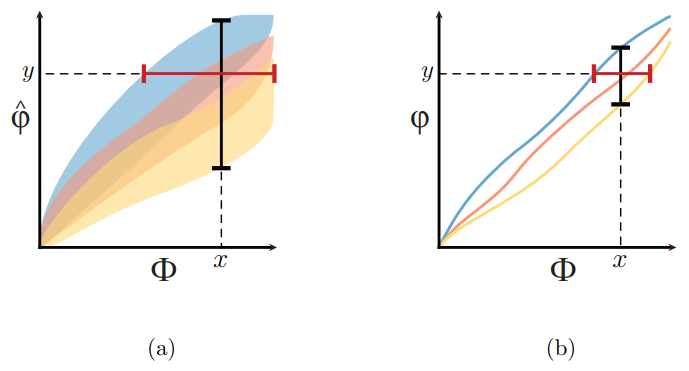
\includegraphics[scale = 0.4]{reshef_2015_fig1.png}
		\caption{
			Una ilustraci\'on esquem\'atica de intervalos confiables e interpretables. En ambas partes de la figura, $\mathcal{Q}$ consiste en relaciones ruidosas de tres tipos diferentes representados en tres colores distintos. (a) La relaci\'on entre un estad\'istico $\hat{\varphi}$ y $\Phi$ en $\mathcal{Q}$ en un tama\~no de muestra finito. Los l\'imites inferior y superior de cada regi\'on sombreada indican los percentiles $(\alpha / 2) \cdot 100 \%$ y $(1 - \alpha / 2) \cdot 100 \%$ de la distribuci\'on de muestreo de $\hat{\varphi}$ para cada tipo de relaci\'on en varios valores de $\Phi$. El intervalo vertical (en negro) es el intervalo confiable $R_\alpha^{\hat{\varphi}}(x)$, y el intervalo horizontal (en rojo) es el intervalo interpretable $I_\alpha^{\hat{\varphi}}(y)$. (b) En el l\'imite de muestra grande, reemplazamos $\hat{\varphi}$ por una cantidad poblacional $\varphi$. El intervalo vertical (en negro) es el intervalo confiable $R^{\varphi}(x)$, y el intervalo horizontal (en rojo) es el intervalo interpretable $I^{\varphi}(y)$.}
		\label{reshef_2015_f1}
	\end{figure}

	\section{Definiendo Equitabilidad}

	\todo{definir $\alpha$-fiabilidad y $\alpha$-interpretabilidad, y finalmente equitatibilidad }

	\subsection[equitabilidadmice]{Equitabilidad del las medidas}

	\todo{esta secci\'on está extraida de la secci\'on en el paper, la idea es hacer un an\'alisis similar para todas medidas propuestas
	}
	
	Como se mencion\'o previamente, una de las principales motivaciones para la introducci\'on de $MIC$ fue la equidad, es decir, hasta qu\'e punto una medida de dependencia captura \'utilmente alguna noci\'on de la fuerza de una relaci\'on en un conjunto de relaciones est\'andar. En esto contexto en Reshef et al. (2016) \cite{Reshef2016} se realiz\~o un an\'alisis emp\'irico de la equidad de $MIC_e$ con respecto a R2 y su desempe\~no fue comparado con la correlaci\'on de distancia (Sz\'ekely et al., (2007)\cite{Szekely2007}; Sz\'ekely and Rizzo, (2009)\cite{Szekely2009}), la estimaci\'on de la informaci\'on mutua (Kraskov et al., 2004) y la estimaci\'on de la correlaci\'on m\'axima (Breiman and Friedman, 1985).

	Se comenz\'o evaluando la equidad en el conjunto de relaciones $Q$ definido anteriormente, un conjunto que ha sido analizado en otros trabajos previos (Reshef et al., 2011, 2015a; Kinney and Atwal, 2014). Los resultados, mostrados en la Figura \ref{reshef_2016_f3}, confirman la superior equidad del estimador $MIC_e$ en este conjunto de relaciones.

	Para evaluar la equidad de manera m\'as objetiva sin depender de un conjunto de funciones curado manualmente, se analizaron 160 funciones aleatorias extra\'idas de una distribuci\'on de proceso Gaussiano con un kernel de funci\'on radial con una de ocho posibles anchuras en el conjunto $\{0.01, 0.025, 0.05, 0.1, 0.2, 0.25, 0.5, 1\}$ para representar una variedad de complejidades de relaciones posibles. Los resultados, mostrados en la Figura \ref{reshef_2016_f4}, muestran que $MIC_e$ supera a los m\'etodos existentes en t\'erminos de equidad con respecto a $R^2$ en estas funciones tambi\'en. Tambi\'en se examin\'o el efecto de las relaciones at\'ipicas en los resultados al muestrear repetidamente subconjuntos aleatorios de 20 funciones de este gran conjunto de relaciones y medir la equidad de cada m\'etodo en promedio sobre los subconjuntos; los resultados fueron similares.

	Una caracter\'istica del desempe\~no de $MIC_e$ en estas relaciones elegidas al azar, como se muestra en la Figura \ref{reshef_2016_f4}, es que parece ser m\'inimamente sensible a la anchura del proceso Gaussiano del cual se extrae una relaci\'on dada. Esto contrasta, por ejemplo, con la estimaci\'on de la informaci\'on mutua, que muestra una sensibilidad pronunciada a este par\'ametro que le impide ser altamente equitativa cuando hay relaciones con diferentes anchuras en el mismo conjunto de datos.

	\begin{figure}[H] 
		\centering
		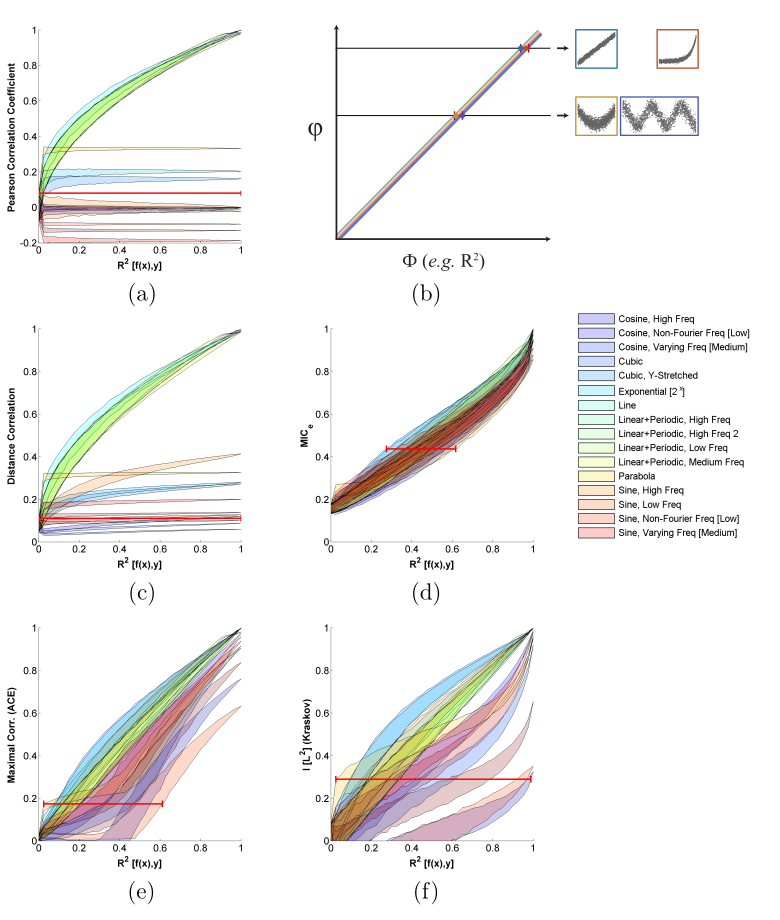
\includegraphics[scale = 0.4]{reshef_2016_fig3.png}
		\caption{Equitabilidad con respecto a $R^2$ en un conjunto de relaciones funcionales ruidosas de $(a)$ el coeficiente de correlaci\~on de Pearson, $(b)$ una medida hipot\~etica de dependencia $\varphi$ con equitabilidad perfecta, $(c)$ la correlaci\~on de distancia, $(d)$ $\mathrm{MIC}_e$, $(e)$ estimaci\~on de correlaci\~on m\~axima y $(f)$ estimaci\~on de informaci\~on mutua. Para cada relaci\~on, una regi\~on sombreada denota los valores estimados en el percentil 5 y 95 de la distribuci\~on muestral de la estad\~istica en cuesti\~on en esa relaci\~on en cada valor de $R^2$. El gr\~afico resultante muestra qu\~e valores de $R^2$ corresponden a un valor dado de cada estad\~istica. El intervalo rojo en cada gr\~afico indica el rango m\~as amplio de valores de $R^2$ que corresponden a un valor de la estad\~istica; cuanto m\~as estrecho sea el intervalo rojo, mayor ser\~a la equitabilidad. Un intervalo rojo con ancho 0, como en $(b)$, significa que la estad\~istica refleja solo $R^2$ sin depender del tipo de relaci\~on, como se demuestra en los pares de miniaturas de relaciones de diferentes tipos con valores id\~enticos de $R^2$.}
		\label{reshef_2016_f3}
	\end{figure}

	\begin{figure}[H] 
		\centering
		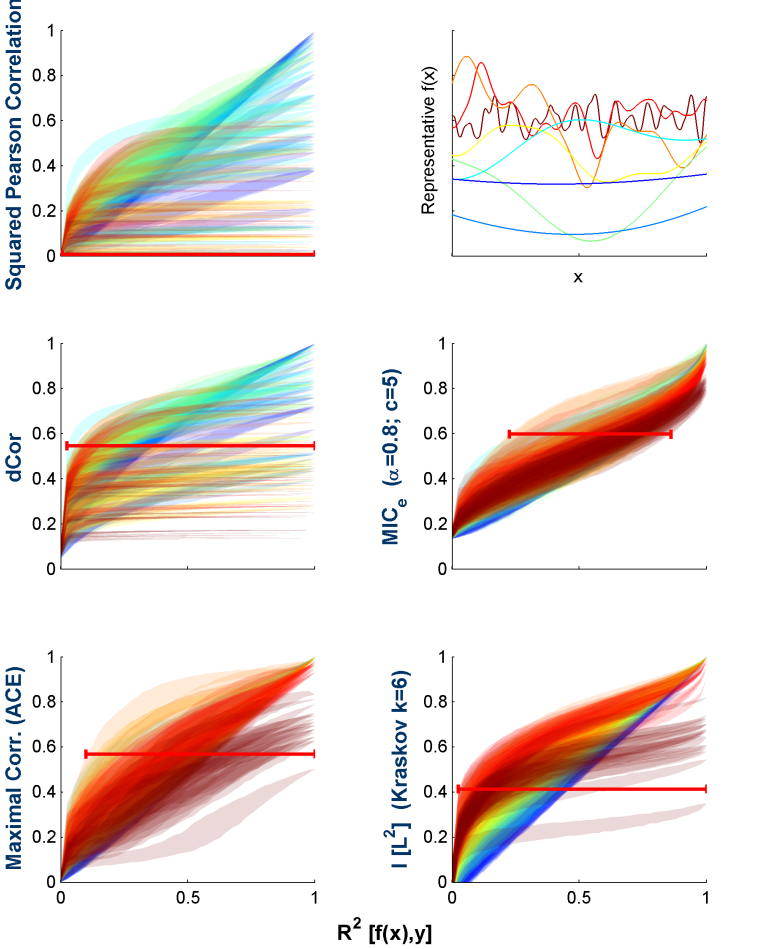
\includegraphics[scale = 0.4]{reshef_2016_fig4.png}
		\caption{Equitabilidad de los m\~etodos examinados en funciones extra\~idas al azar de una distribuci\~on de proceso gaussiano. Cada m\~etodo se eval\~ua como se muestra en la Figura \ref{reshef_2016_f3}, con un intervalo rojo que indica el rango m\~as amplio de valores de $R^2$ correspondiente a cualquier valor de la estad\~istica; cuanto m\~as estrecho sea el intervalo rojo, mayor ser\~a la equitabilidad. Cada regi\~on sombreada corresponde a una relaci\~on, y las regiones est\~an coloreadas seg\~un el ancho de banda del proceso gaussiano del que se muestrearon. Las relaciones de muestra para cada ancho de banda se muestran en la esquina superior derecha con colores correspondientes.}
		\label{reshef_2016_f4}
	\end{figure}
\blankpage
% ---------------------------------------------------------------------------------------
\chapter{Comprarando una Imgaen con su tranformada}\label{chap5}

\section{Introducci\'on}

    Como ya mencionamos en el cap\'itulo \ref{chap4} se utilizaron im\'agenes de la base de datos ''\textit{Kodak Lossless TrueColor Image Suite}''\ref{fig:rgb2gray_2} \cite{KodakLosslessTrueColorImageSuite}. A cada una de las correspondientes im\'agenes ser\'an pasadas a blanco y negro, como fue descrito en \ref{eq:grayscale}, y posteriormente se le aplicar\'a la transformaci\'on de Box-Cox con los tr\'es m\'etodos de selecci\'on de $\lambda$ descritos en el cap\'itulo anteror.

    \begin{figure}[H]
        \centering
        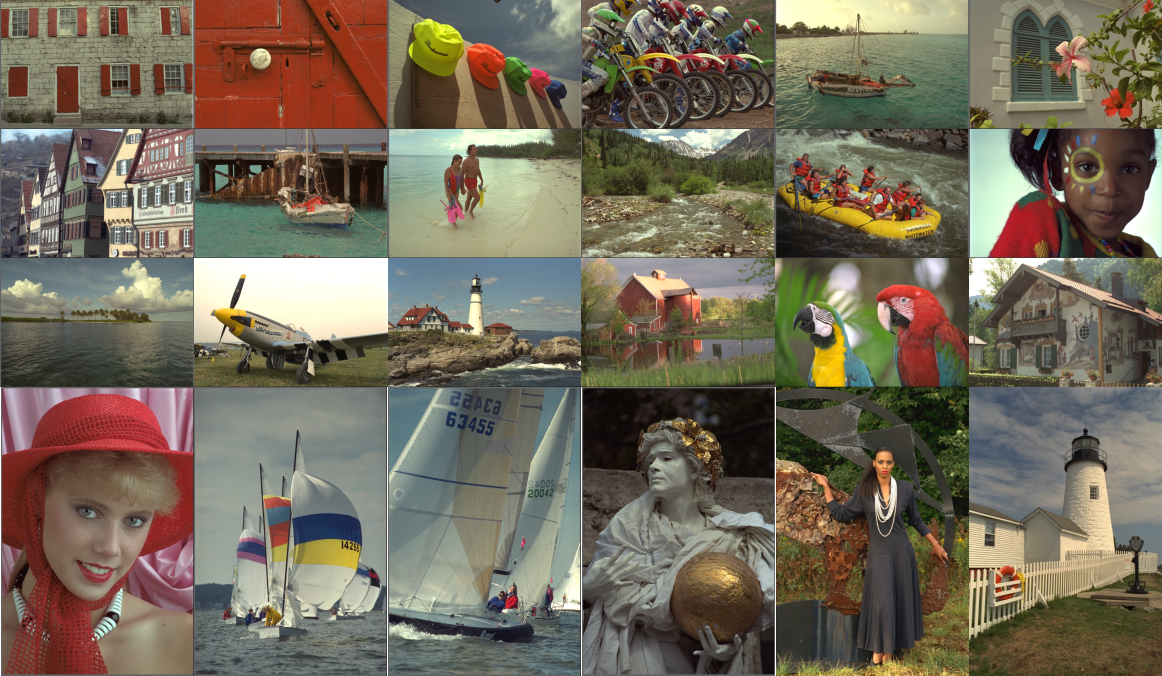
\includegraphics[width=0.5\textwidth]{all_images_grid.png}
        \caption{Banco de imagenes en blanco y negro.}
        \label{fig:rgb2gray_2}
    \end{figure}
    
    Ya revisamos el efecto que en general tiene cada $\lambda$ en la im\'agen, y como la selecci\'on de este afecta a cada una, en la siguientes secci\'ones discutiremos la relaci\'on que existe entre una im\'agen y su transformada para $\lambda$ cualquiera en el conjunto $[-2, 5]\subset\R$ y posteriormente como se ve la relaci\'on entre una im\'agen y su transformada usando los distintos lamdba entregados 
    
\section[Comparando imagenes vs. lambda]{Comparando imagenes vs. $\lambda$}

    Antes de comparar las im\'agenes con su tranformada dado el $\lambda$ eleguido por algunos de los m\'etodos estudiados, queremos revisar si hay una relaci\'on com\'un entre las im\'agnes y su transformada para un $\lambda$ cualquiera en $[-2, 5]\subset\R$. Veamos los resultados \todo{ref figura, crear una solo figura con todo}. Veamos primero los resultados sobre las im\'agenes completas


    \begin{figure}[H]
        \centering
        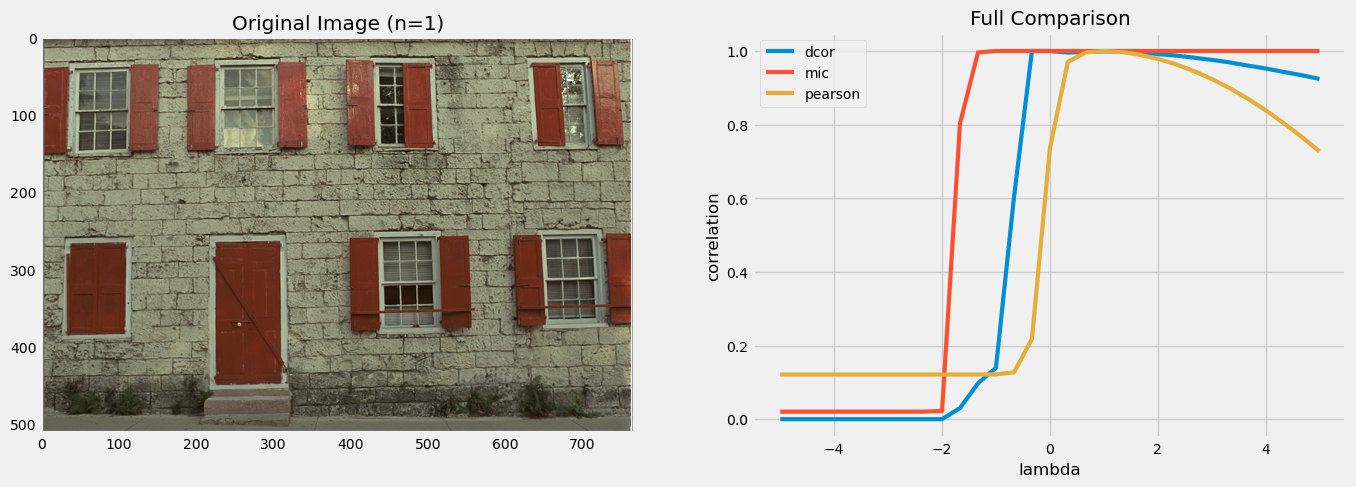
\includegraphics[width=0.5\textwidth]{lam_v_com_1.png}
        \caption{Im\'agen 1 junto con su correlaci\'on vs. $\lambda$}
    \end{figure}

    \begin{figure}[H]
        \centering
        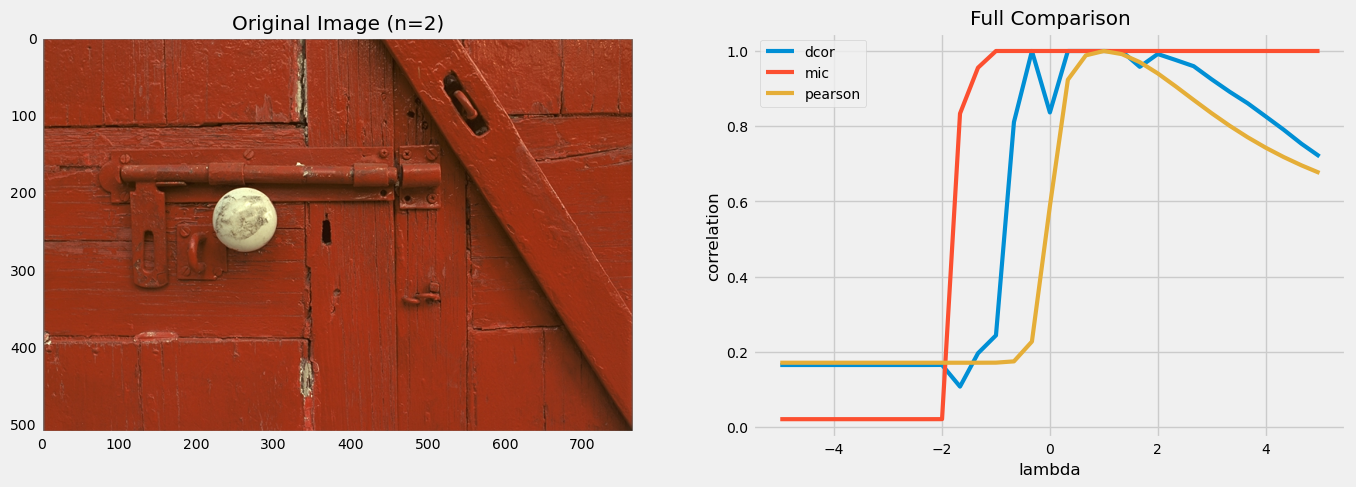
\includegraphics[width=0.5\textwidth]{lam_v_com_2.png}
        \caption{Im\'agen 2 junto con su correlaci\'on vs. $\lambda$}
    \end{figure}

    \begin{figure}[H]
        \centering
        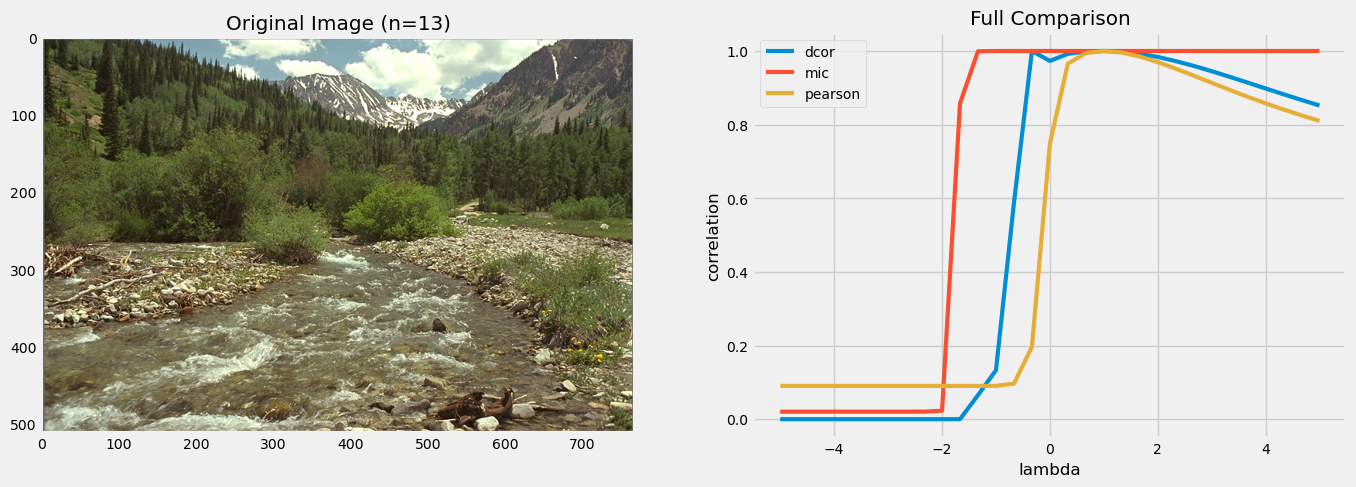
\includegraphics[width=0.5\textwidth]{lam_v_com_13.png}
        \caption{Im\'agen 13 junto con su correlaci\'on vs. $\lambda$}
    \end{figure}

    \begin{figure}[H]
        \centering
        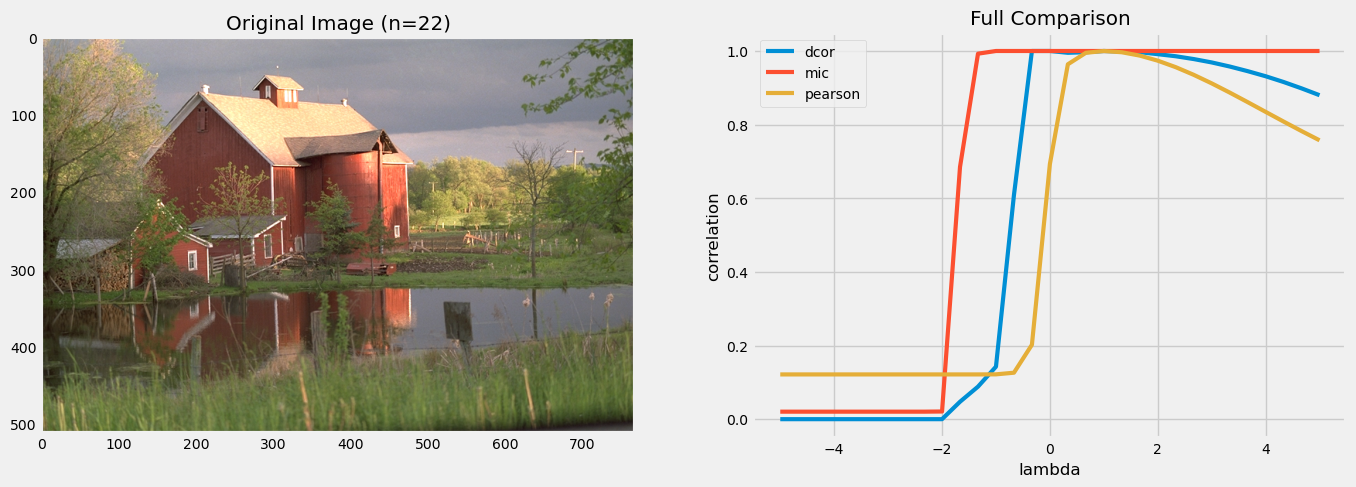
\includegraphics[width=0.5\textwidth]{lam_v_com_22.png}
        \caption{Im\'agen 22 junto con su correlaci\'on vs. $\lambda$}
    \end{figure}

    Podemos ver que todas las curvas se comportan de forma similar, pero cabe descatar que el el MIC el cual detecta la relaci\'on de forma m\'as temprana, con dCor siguiendo no mucho m\'as atr\'as. Otra cosa que vale la pena mencionar es que el MIC mantiene una correlaci\'on alta con la im\'agen original, incluso para valores altos de $\lambda$, cosa que no ocurre con dCor, el cual disminuyemientas los valores de $\lambda$ van aumentando.

    Repitiendo lo anterior, pero ahora con el m\'etodo del histograma tenemos: 

    \begin{figure}[H]
        \centering
        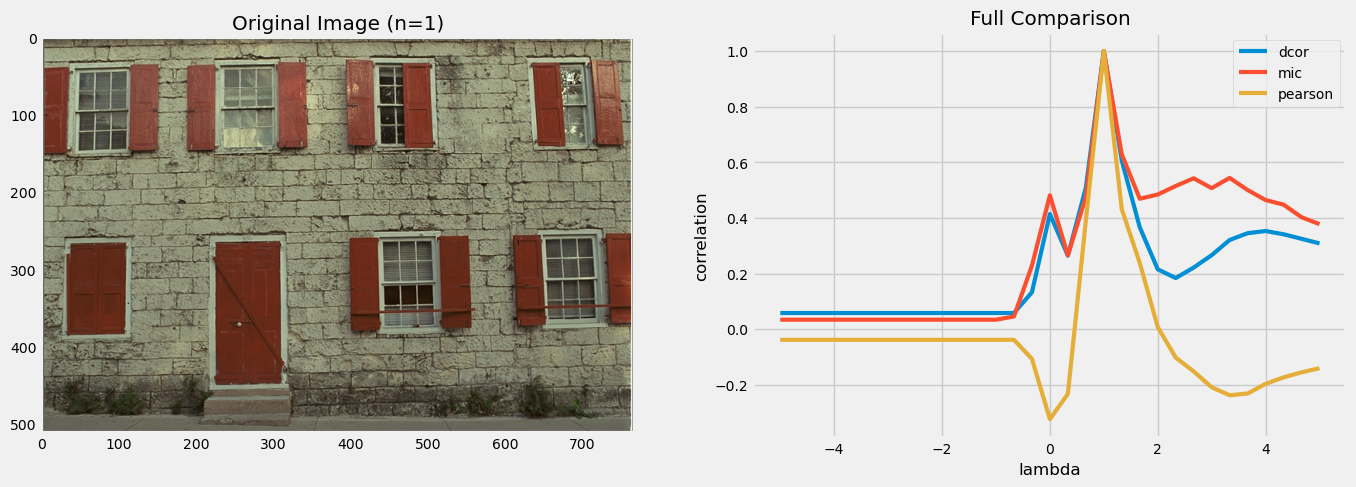
\includegraphics[width=0.5\textwidth]{lam_v_com_1_hist.png}
        \caption{Im\'agen 1 junto con su correlaci\'on vs. $\lambda$}
    \end{figure}

    \begin{figure}[H]
        \centering
        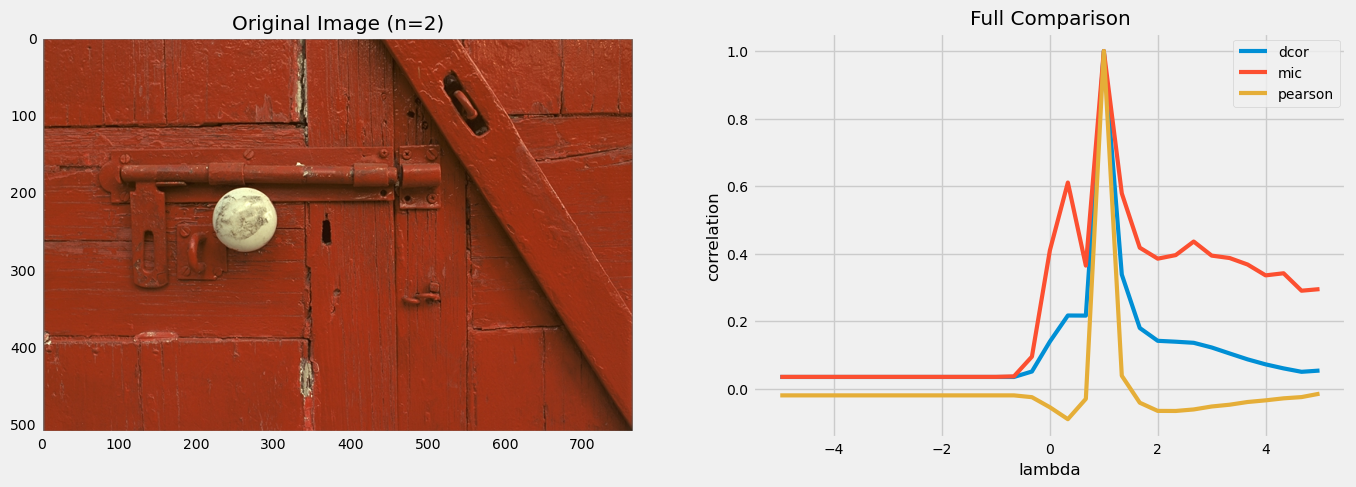
\includegraphics[width=0.5\textwidth]{lam_v_com_2_hist.png}
        \caption{Im\'agen 2 junto con su correlaci\'on vs. $\lambda$}
    \end{figure}

    \begin{figure}[H]
        \centering
        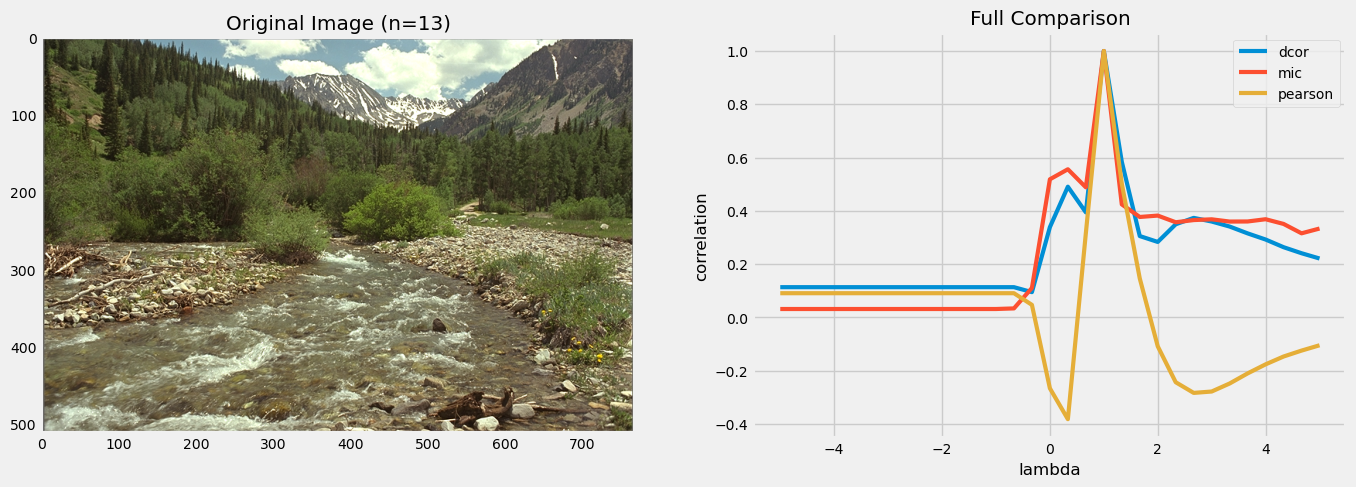
\includegraphics[width=0.5\textwidth]{lam_v_com_13_hist.png}
        \caption{Im\'agen 13 junto con su correlaci\'on vs. $\lambda$}
    \end{figure}

    \begin{figure}[H]
        \centering
        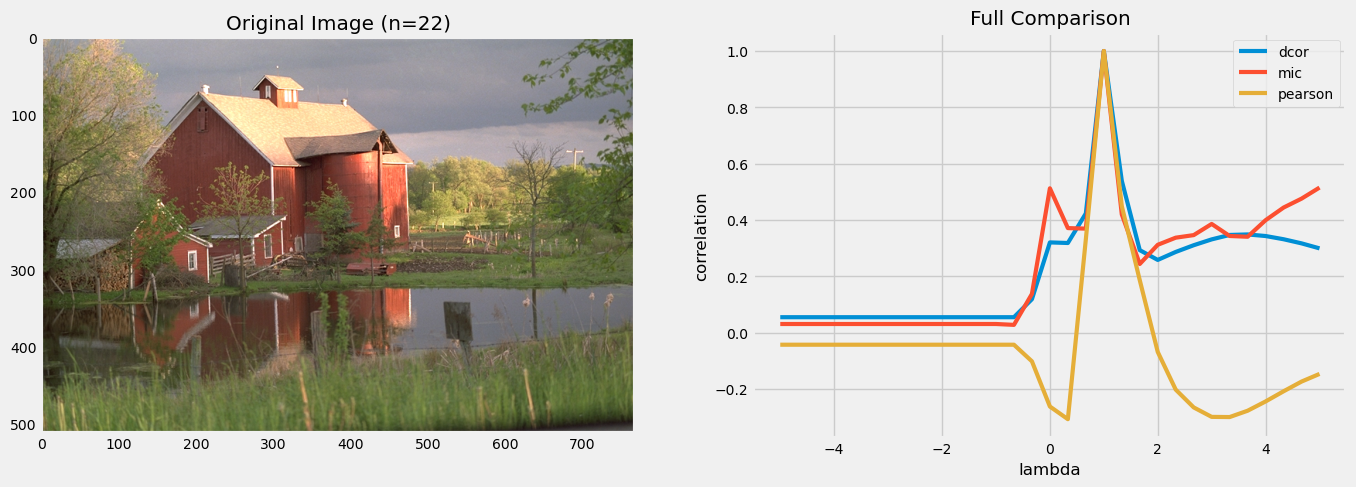
\includegraphics[width=0.5\textwidth]{lam_v_com_22_hist.png}
        \caption{Im\'agen 22 junto con su correlaci\'on vs. $\lambda$}
    \end{figure}

    Podemos ver que tenemos un efecto similar, \todo{ampliar conclusion}



\section{Comparando imagenes con su tranformada}
todo{necesita un mejor titulo}

    \todo{todo esto}

    Esta es la parte en la que comparamos el valor de la correlaci\'on entre la im\'agen y su transformada para cada m\'etodo de selecci\'on de $\lambda$. 

    Es en donde m\'as dudas tengo sobre concluir, que mencionar, etc. dejo un resumen de los resultados y quedo atento a los compentarios
    
    Al comparar las imagenes suando sus histogramas obtener los siguientes promedios (full, hist y grid se refieren al m\'etodo de selecci\'on de $\lambda$)

    \begin{table}[H]
        \begin{tabular}{ll}
        mic\_full     & 0.483314  \\
        dcor\_full    & 0.453417  \\
        mic\_hist     & 0.450874  \\
        dcor\_hist    & 0.424125  \\
        mic\_grid     & 0.409863  \\
        dcor\_grid    & 0.357291  \\
        pearson\_full & 0.161884  \\
        pearson\_grid & 0.114137  \\
        pearson\_hist & -0.233827 \\
        pearson\_hist & -0.233827
        \end{tabular}
    \end{table}

    noteamos que la mayor relacion la encontramos al usar toda la imagen parabuscar un lamdba

    en el caso de comparar las imagenes usando todo el vector, tenemos

    \begin{table}[H]
        \begin{tabular}{ll}
        dcor\_full    & 1.000000  \\
        mic\_full     & 1.000000  \\
        mic\_hist     & 1.000000  \\
        pearson\_full & 0.987437  \\
        mic\_grid     & 0.970955  \\
        dcor\_hist    & 0.947233  \\
        pearson\_hist & 0.924601  \\
        pearson\_hist & 0.924601  \\
        dcor\_grid    & 0.865844  \\
        pearson\_grid & 0.842625  \\
        pearson\_hist & -0.233827
        \end{tabular}
    \end{table}

    en donde vemos que la mayor relaci\'on la encontramos al usar todo el vector para buscar un $\lambda$, pero no es muy distinto a usar el histograma.

    En general usar grid para buscar un $\lambda$ es el peor m\'etodo, pero no es muy distinto a usar el histograma.

    Veamos como se ven los valores para cada imagen, primero comparando los histogramas y luego comparando todo el vector

    \begin{figure}[H]
        \centering
        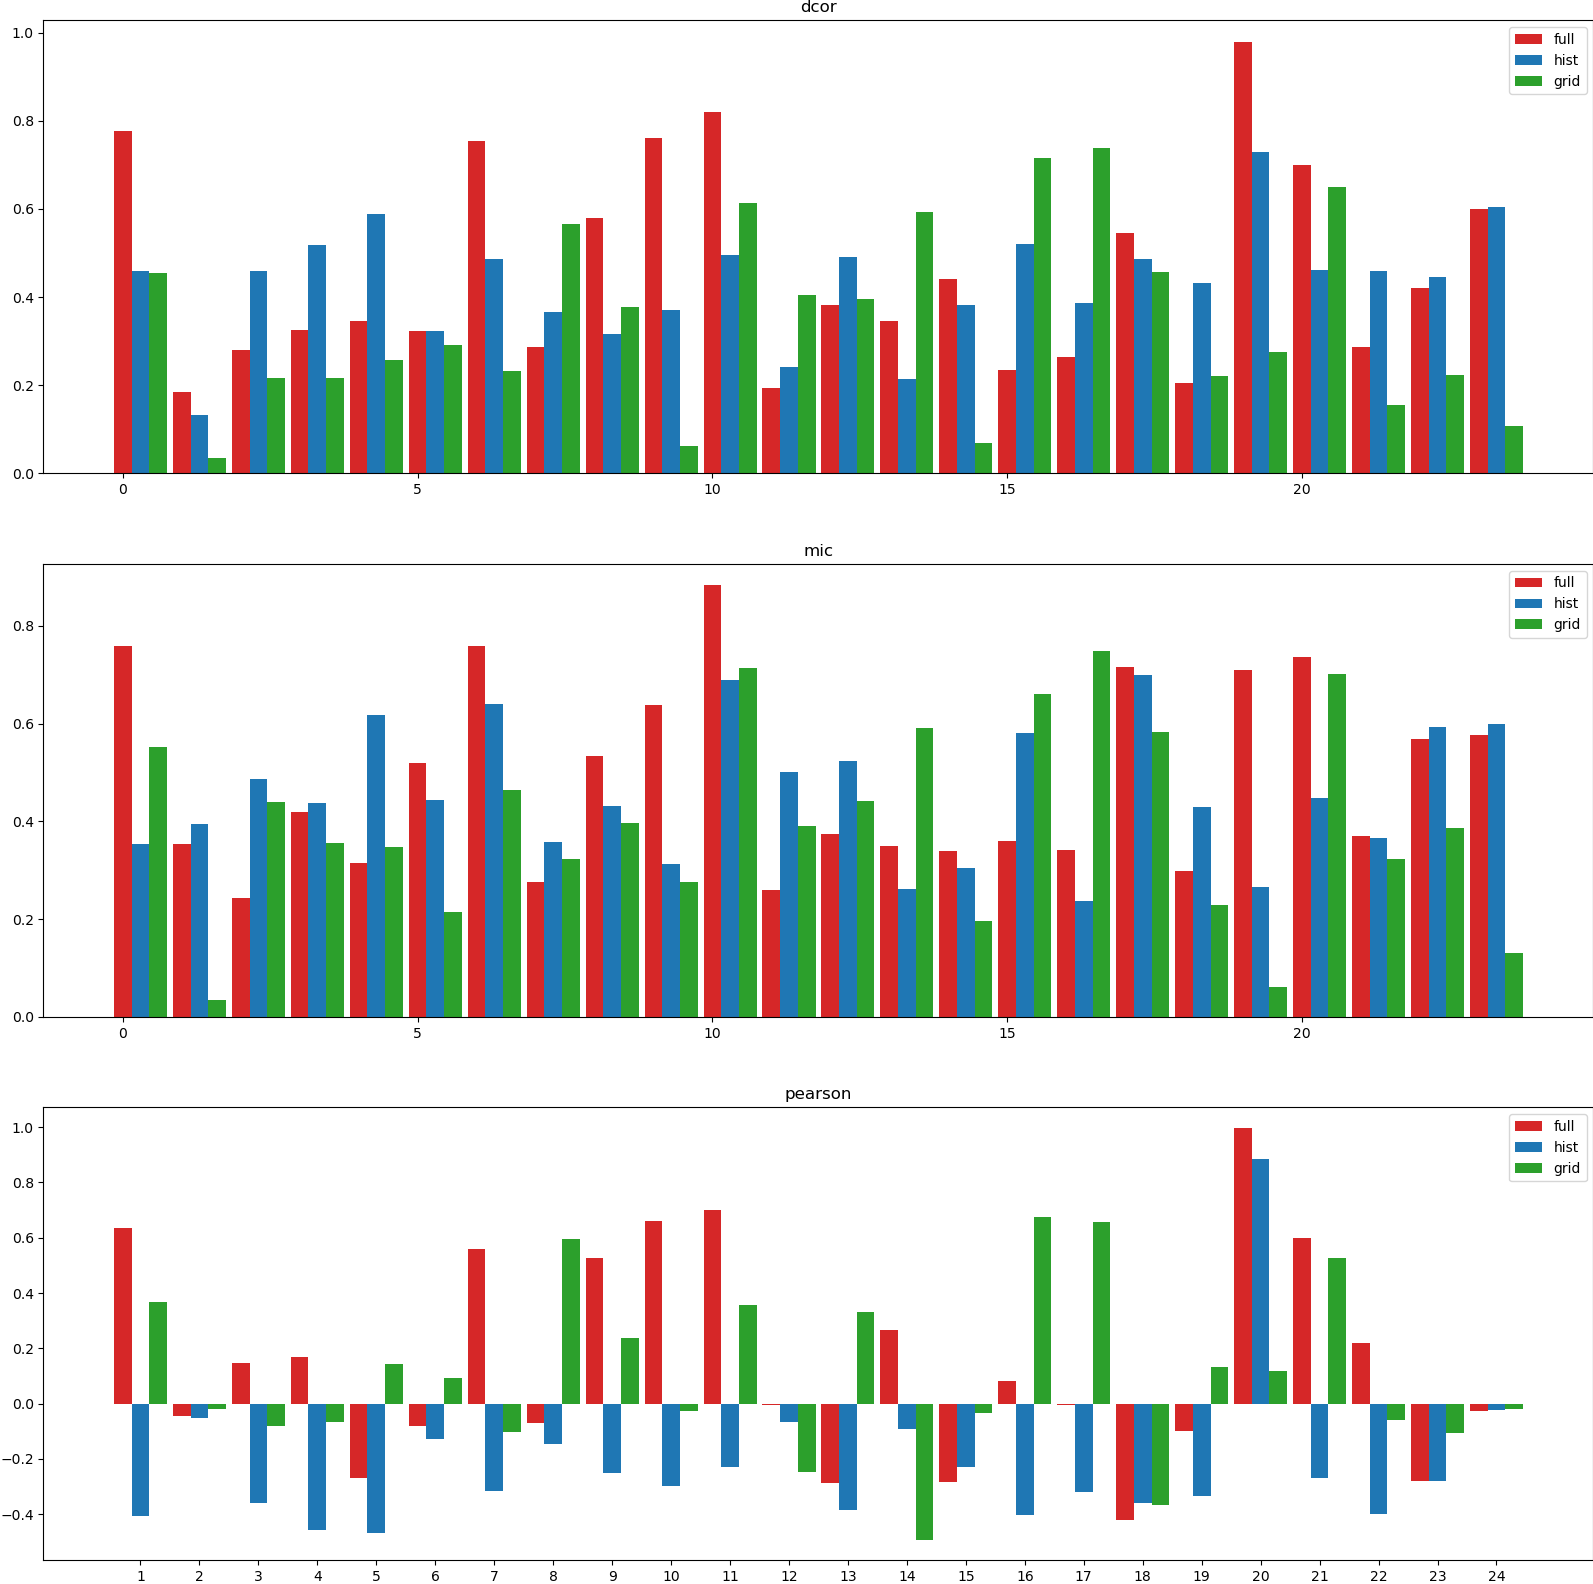
\includegraphics[width=0.6\textwidth]{plot_comparison_hist.png}
        \caption{Valores de dcor, mic y pearson para cada imagen usando el histograma, azul es el metodo para encontrar $\lambda$ con toda la imagen, rojo es el histograma y amarillo es el grid}
    \end{figure}


    \begin{figure}[H]
        \centering
        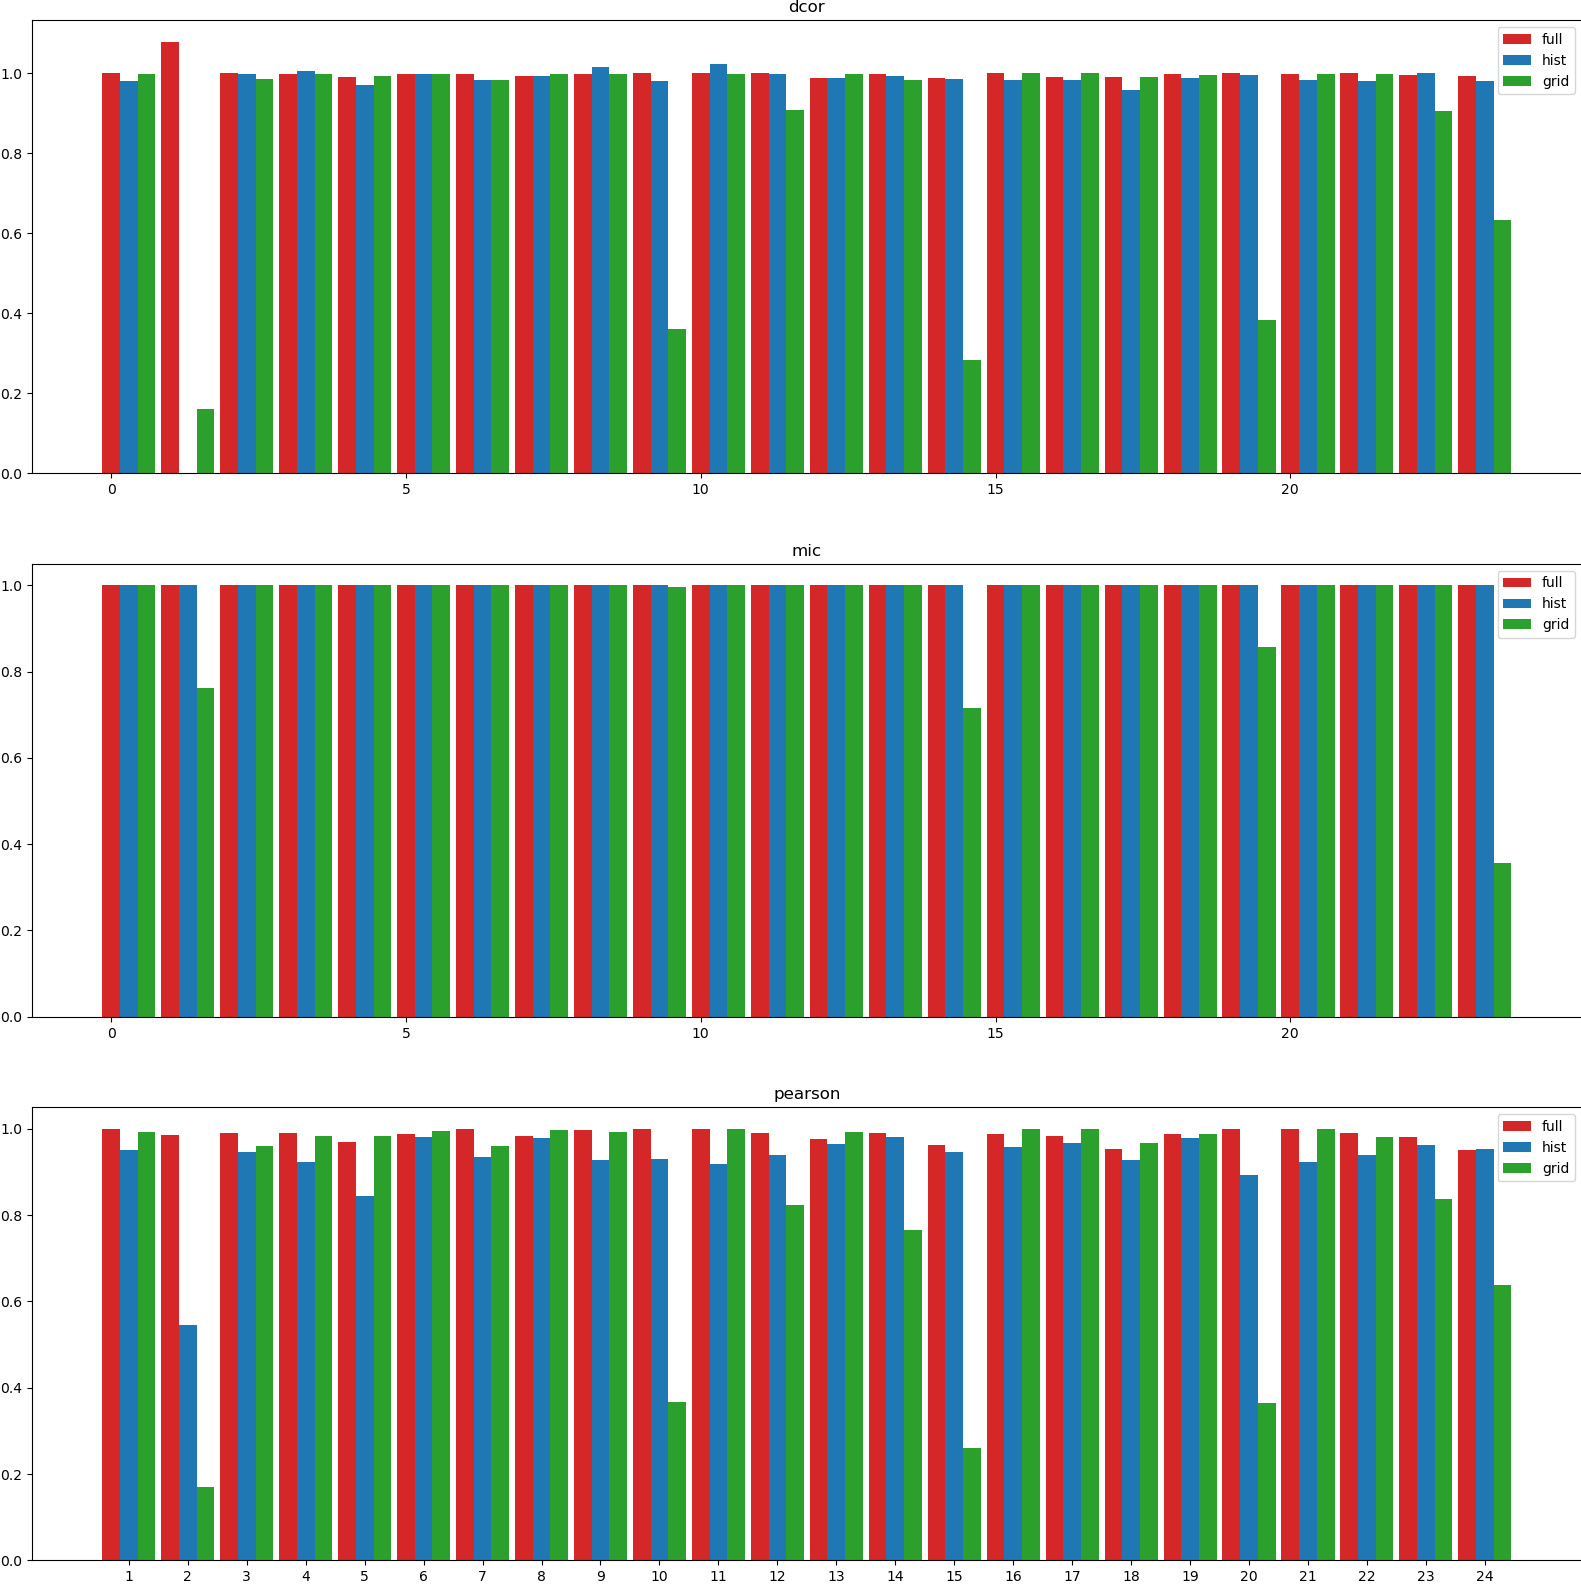
\includegraphics[width=0.6\textwidth]{plot_comparison_full.png}
        \caption{Valores de dcor, mic y pearson para cada imagen usando todo el vector, azul es el metodo para encontrar $\lambda$ con toda la imagen, rojo es el histograma y amarillo es el grid}
    \end{figure}

\section{Concluciones}

\todo{concluir}
\blankpage
% ---------------------------------------------------------------------------------------
\chapter{La transformaci\'on de Box y Cox}\label{chap6}

    \section{Introducci\'on}
 
    La transformaci\'on de Box y Cox, conocida como Box-Cox, es una t\'ecnica de transformaci\'on no lineal que fue propuesta por George Box y David Cox en 1964 en su trabajo \textit{''An Analysis of Transformations''}\cite{boxcox64}. Cuenta la historia que el Profesor cox estaba visitando al doctor Box en Wisconsin, y decidieron que deberían escribir un artículo juntos dada la similitud de sus nombres, y que ambos eran británicos \cite{lane2003introduction}. 
    Muchos importantes resultados y t\'ecnicas en el an\'alisis estad\'istico de datos toman el supuesto de que los datos poseen una distribuc\'on normal, en los casos cuando este supuesto no se sostiene, una de las alternativas es transformar los datos para que se acerquen a una distribuci\'on normal. En este contexto la transformaci\'on de Box-Cox fue propuesta para convertir un conjunto de datos en una distribuci\'on que se asemeja a la normal, dejando una distribuci\'on con menos sesgo que es un poco m\'as sim\'etrica, esto suele ser determinado en base a un test de m\'axima verosimilitud, m\'as adeltante discutiremos el motivo de esto. La transformaci\'on de Box-Cox pertenece una familia de t\'ecnicas conocidas como transformaciones de potencia. Estas transformaciones buscan modificar los datos de entrada elev\'andolos a una potencia determinada, identificada por el par\'ametro $\lambda$.
    
    Box y Cox desarrollaron este m\'etodo con la intenci\'on de crear una t\'ecnica de transformaci\'on flexible que pudiera adaptarse a diversas distribuciones de datos, esto permite adaptar el coeficiente para funcionar en distintos contextos, y de nuestro interes particular es en el contexto de im\'agenes. En general la transformaci\'on solo es utilizada sobre vectones 1-dimensional. En 2020 Abbas Cheddad p\'ublico \textit{''On Box-Cox Transformation for Image Normality and Pattern Classification''}\cite{boxcoximg}, donde se discut\'io el coeficiente como un paso de preprocesamiento de im\'agenes, tanto para mejoramiento visual, como para mejorar el desempe\~no de algoritmos de clasificaci\'on. En este trabajo se propuso una nueva forma de aplicar la transformaci\'on, que consiste en utilizar el histograma de la imagen como proxy comprimido de la matriz de datos, y as\'i poder aplicar la transformaci\'on de forma r\'apida.
    
    En este cap\'itulo vamos a discutir la transformaci\'on de Box-Cox, presentaremos su definici\'on, y discutiremos el motivo de su uso. Luego vamos a discutir el trabajo de Cheddad\cite{boxcoximg}, y como este puede ser aplicado sobre imagenes. Finalmente discutiremos alternativas para calcular $\lambda$ sobre im\'agenes.
    
    \section{Definiciones}
    Para un $\lambda\in\R$ dado, la transformaci\'on de Box-Cox se define como:
    \begin{equation}\label{Box-Cox}
        y^{(\lambda)}= \begin{cases}\frac{y^{\lambda}-1}{\lambda} & (\lambda \neq 0) \\ \log y & (\lambda=0)\end{cases}
    \end{equation}
    
    $\forall y\in\R_{>0}$. En la pr\'actica los valores de $\lambda$ se restringen a un intervalo, normalmente $[-2,2]$ o $[-5,5]$, notemos adem\'as que en la practica se toma la segunda forma cuando $|\lambda|<0.01$\cite{boxcoximg}.
    
    Adem\'as existe una versi\'on para datos no positivos dada por:

    $$
    y^{(\lambda)}= \begin{cases}\frac{\left(y+\lambda_{2}\right)^{\lambda_{1}}-1}{\lambda_{1}} & \left(\lambda_{1} \neq 0\right), \\ \log \left(y+\lambda_{2}\right) & \left(\lambda_{1}=0\right) .\end{cases}
    $$

    Esta versi\'on es menos utilizada en la pr\'actica, dado que se suelen realizar otros pasos de preprocesamiento que dejan los datos entre 0 y 1.
    
    Cabe notar que Bicego y Baldo (2016)\cite{bicego2016} demostraron que, dado un vector $\textbf{y}=(y_1,\dots,y_n)\in\R^n_{>0}$, la transformaci\'on no cambia dado el orden de los elementos en el vector, por lo tanto al momento de aplicar la transformaci\'on sobre una imagen, o en general una matriz d-dimensional, se puede aplicar la cualquier ordenamiento sobre los datos, y luego aplicar la transformaci\'on sobre el vector unidimensional resultante. Dado esto tambi\'en cabe notar que al ser agn\'ostica con respecto al orden de los datos, la transformaci\'on no altera la relaci\'on espacial entre los datos.
    
    Este no es el caso para la definici\'on de lambda, que es lo que discutiremos en la siguiente secci\'on.

    \section[eliguiendo lambda]{Elguiendo $\lambda$}

    Como mencionamos anteriormente, el objetivo de la transformaci\'on es encontrar el valor de $\lambda$ que proporciona el mejor ajuste a una distribuci\'on normal. Para esto, Box y Cox proponen un criterio de m\'axima verosimilitud, el cual se define como:

    \begin{equation}
        \mathcal{L}(\lambda) \equiv-\frac{n}{2} \log \left[\frac{1}{n} \sum_{j=1}^{n}\left(x_{j}^{\lambda}-\overline{x^{\lambda}}\right)^{2}\right] +(\lambda-1) \sum_{j=1}^{n} \log x_{j}
    \end{equation}
    donde $\overline{x^{\lambda}}$ es el promedio muestral del vector transformado.

    La verosimilitud juega un papel crucial en el proceso de transformaci\'on de Box-Cox. En t\'erminos simples, la verosimilitud se refiere a la probabilidad de que un conjunto de datos observados se derive de una distribuci\'on estad\'istica particular. En este caso, la verosimilitud se utiliza para medir qu\'e tan bien una distribuci\'on normal se ajusta a los datos transformados para diferentes valores de $\lambda$. El valor de $\lambda$ que maximiza esta verosimilitud es el que se selecciona para la transformaci\'on.

    
    La transformaci\'on de Box-Cox persigue un objetivo esencial en el an\'alisis estad\'istico: garantizar el cumplimiento de los supuestos necesarios para la aplicaci\'on de modelos lineales. Esta garant\'ia posibilita el uso de t\'ecnicas de an\'alisis de varianza est\'andar en los datos transformados. En este sentido, Bicego y Bald\'o \cite{bicego2016} resaltan que esta transformaci\'on no altera el ordenamiento de los datos, manteniendo intacta la relaci\'on inherente entre ellos.

    Es importante aclarar, sin embargo, que no todos los conjuntos de datos pueden ser transformados de tal manera que resulten en una distribuci\'on normal perfecta. A pesar de esta limitaci\'on, Draper y Cox \cite{draper1969}argumentan que la transformaci\'on de potencia puede ser efectiva en muchos casos. Incluso en situaciones donde la transformaci\'on no logra una normalidad exacta, las estimaciones habituales del par\'ametro $\lambda$ pueden desempe\~nar un papel vital en la regularizaci\'on de los datos.

    Este proceso de regularizaci\'on conduce a una distribuci\'on que cumple con ciertos criterios deseables, como la simetr\'ia o la homocedasticidad. Esta \'ultima caracter\'istica, que se refiere a la constancia de la varianza a lo largo del conjunto de datos, es especialmente \'util en campos como el reconocimiento de patrones y el aprendizaje autom\'atico. Por ejemplo, en el an\'alisis discriminante lineal de Fisher, la homocedasticidad facilita la diferenciaci\'on entre diferentes clases de datos, potenciando la eficacia de este tipo de t\'ecnicas de aprendizaje autom\'atico.


    \section[]{Box-Cox sobre imagenes} 

    En su art\'iculo del 2020 \cite{boxcoximg}, Abbas Cheddad resalta una notable brecha en la aplicaci\'on de la transformaci\'on de Box-Cox a im\'agenes digitales. Seg\'un Cheddad, existe una carencia significativa de estudios en este \'ambito, destacando el trabajo de JD Lee en 2009 como una excepci\'on\cite{lee2009mr}. En el estudio de Lee, se present\'o un m\'etodo de segmentaci\'on para im\'agenes de resonancia magn\'etica cerebral a trav\'es de una t\'ecnica de transformaci\'on de distribuci\'on. En este enfoque, la transformaci\'on de Box-Cox se aplic\'o a las im\'agenes de resonancia magn\'etica cerebral para normalizar la distribuci\'on de intensidad de los p\'ixeles. Es relevante se\~nalar que, en este estudio, las im\'agenes se trataron como un vector de datos en lugar de una matriz, lo que implica un enfoque unidimensional en la manipulaci\'on y an\'alisis de la imagen.

    Cabe destacar que el proceso de aplicar la tranformaci\'on es iterativo, en el cual se ha de buscar un parametro $\lambda$, esto hace que aplicar esta la transformaci\'on en grandes bancos de imagenes sea demoroso. Una alternativa propuesta por A. Cheddad \cite{boxcoximg} es utilizar el histograma como proxy comprido de la matriz de datos, dado que este refleja la probabilidad estimada de que un pixel esa de un tono en particular. En lo que continua de la secci\'on discutiremos este m\'etodo.

    Dada una imagen en el espacio de color RGB, como fue defininda en el cap\'itulo \ref{chap5}, definimos:
    
    $$
    \mathcal{F}(u, v)=\{R(u, v), G(u, v), B(u, v)\}
    $$

    donde $(u, v)$ son las coordenadas en el espacio de pixeles que cumplen $u=1, \ldots U$, $v=1, \ldots V$ y $(U, V)$ son las dos dimensiones de la foto. Notemos que cada elemento de la imagen es vector de tres dimensiones con los canales rojo, verde, y azul, pero en la literatura se suele trabajar con imagenes en escala de grises, para esto utilizaremos la siguiente formula.

    $$
    \mathcal{F}^{\prime} =(0.299 \mathrm{R}+0.587 \mathrm{G}+0.114 \mathrm{~B})
    $$

    Que corresponde al canal de escala de grises como est\'a definido por el espacio de color $\mathrm{YC}_{\mathrm{b}} \mathrm{C}_{\mathrm{r}}$ lo calcula. En la figrua 
    
    Ahora, antes de pasar a la siguiente secci\'on, podemos ver algunos ejemplos de como afecta a una imagen la aplicaci\'on de la transformaci\'on a lo largo de un rango de valores para $lambda$. En la

    \section[prpuestas de lambda]{Propuestas de $\lambda$ para imagenes.}\label{}

    En base a esto definimos la funci\'on de probabilidad de im\'agen, i.e., el histograma como:
    
    $$\chi(i)=\sum_{i=0}^{255}\mathcal{F}^{\prime}_i,$$

    donde $i$ es el nivel de gris.
    
    Ahora, denotemos por $\hat{\lambda}_{\chi}$ al parametro de la transformaci\'on Box-Cox seleccionado usando el histograma, y de forma analoga definamos $\lambda_{\mathcal{F}^{\prime}}$ al seleccionado usando los datos completos. Fue obserado por Cheddad que estos no coinciden (de hecho la correlaci\'on entre estos es $r^2=-0.3022$) pero aun as\'i este calculo se ha desmostrado util en problemas de clasificaci\'on.

    Ahora definimos $\mathcal{F}^{\prime}(u, v)^{\lambda_{\chi}}$ como los datos siendo aplicada la transformaci\'on Box-Cox definida en (\ref{Box-Cox}), y por ultimo vamos a definir Box-Cox para imagenes o BCI como:

    $$    
    \begin{aligned}
        &B C I=\frac{\left(\mathcal{F}^{\prime \prime}(u, v)-\min \left(\mathcal{F}^{\prime \prime}(u, v)\right)\right)}{\left(\max \left(\mathcal{F}^{\prime \prime(u, v)}\right)-\min \left(\mathcal{F}^{\prime \prime(u, v)}\right)\right)}\\
        &\text { con } \mathcal{F}^{\prime \prime}(u, v)=\mathcal{F}^{\prime}(u, v)^{\hat{\lambda}_{\chi}}
    \end{aligned}
    $$
    
    Notemos que este ultimo paso se realiza para que los datos esten entre 0 y 1, y as\'i poder ser representados en una imagen. En la Figura se puede ver un ejemplo de la transformaci\'on aplicada sobre una imagen, con ambas versiones de $\lambda$.


    

\blankpage
\appendix
% ---------------------------------------------------------------------------------------
\chapter{Resultados sobre el banco de im\'agenes}\label{appA}

En este ap\'endice incluimos los resultados obtenidos sobre el banco de im\'agenes, para los distintos experimentos y otras figuras de interes. 


\begin{figure}[H]
    \centering
    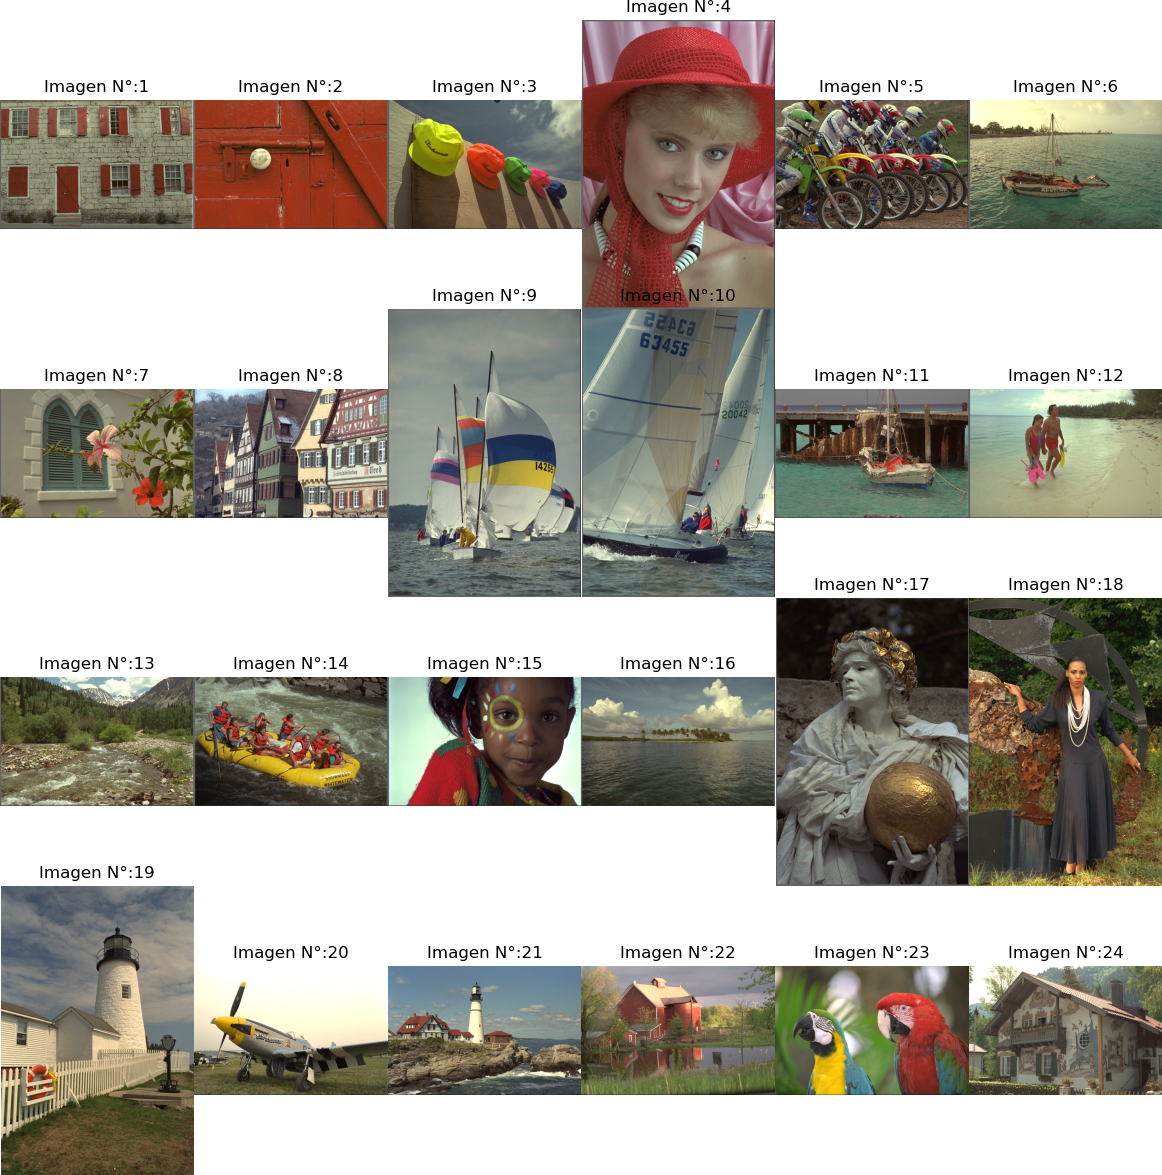
\includegraphics[width=0.7\textwidth]{figuras/all_images_in_order.png}
    \caption{imagenes en el orden original del Banco.}
\end{figure}


\begin{figure}
    \centering
    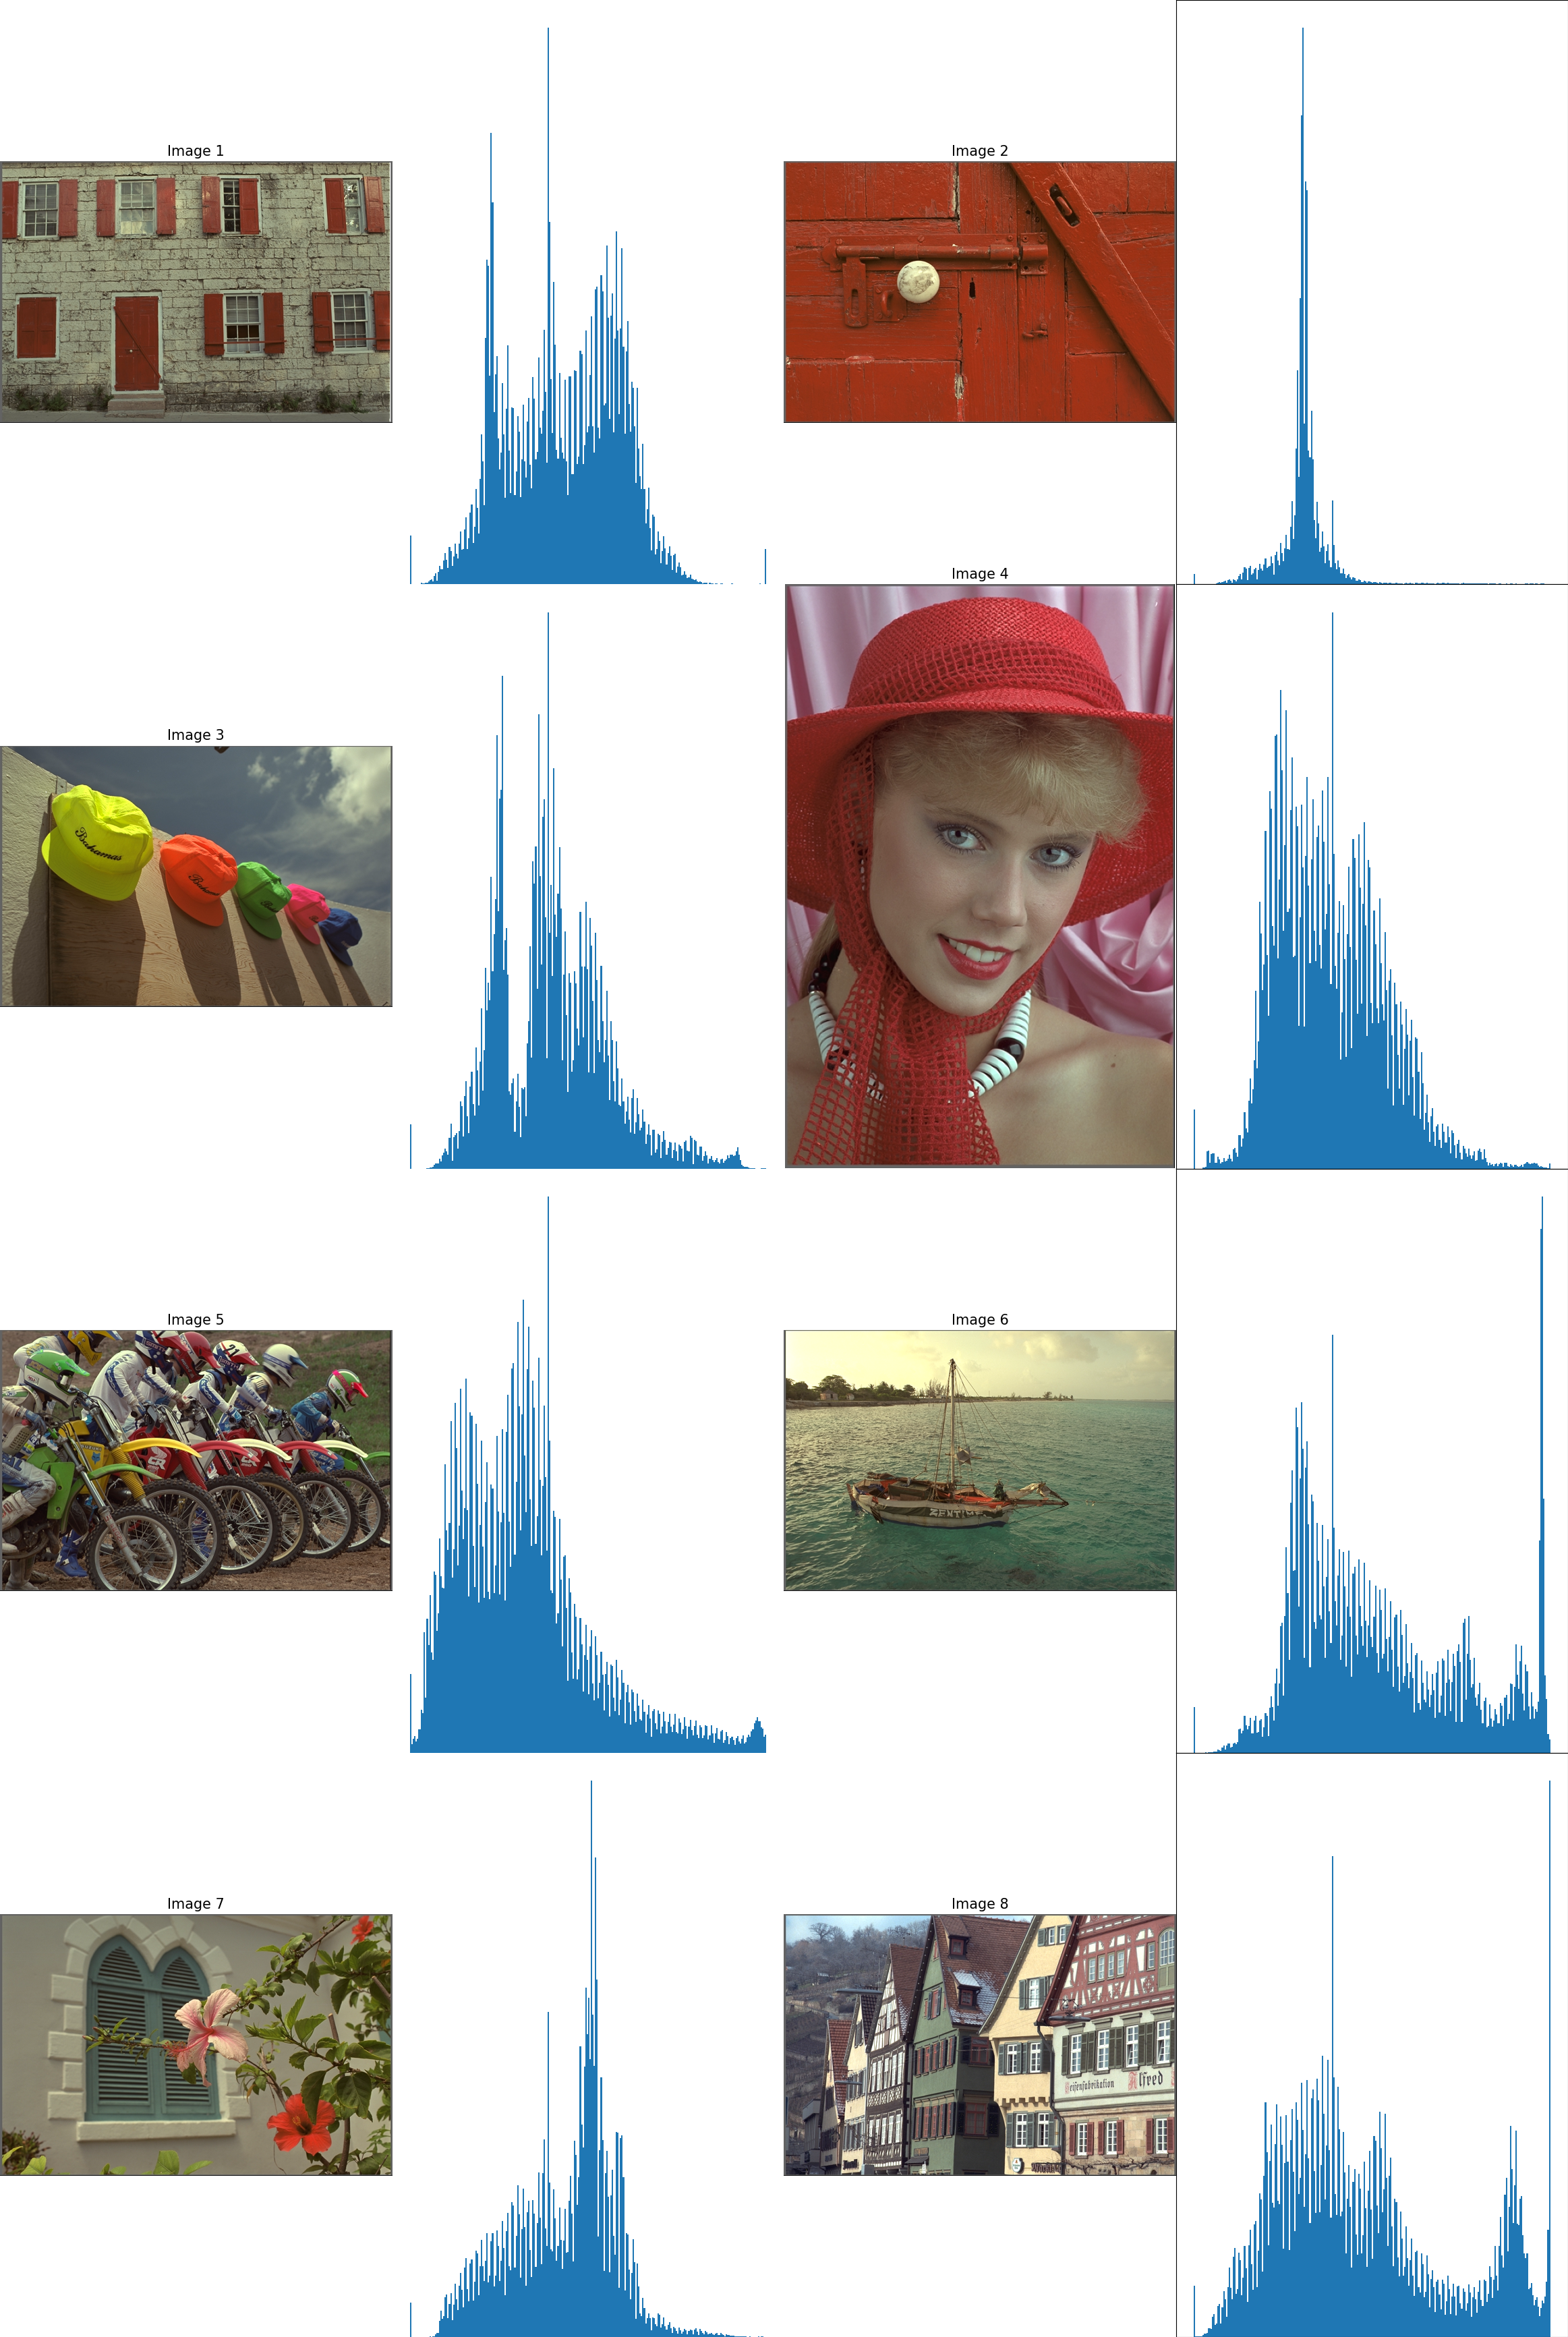
\includegraphics[width=0.8\textwidth]{figuras/img_hist_1.png}
    \caption{Imagen original e histomgrama para todas imagenes del banco, en orden im\'agen 1 hasta 8.}
\end{figure}

\begin{figure}
    \centering
    \includegraphics[width=0.8\textwidth]{figuras/img_hist_2.png}
    \caption{Imagen original e histomgrama para todas imagenes del banco, en orden im\'agen 9 hasta 16.}
\end{figure}

\begin{figure}
    \centering
    \includegraphics[width=0.8\textwidth]{figuras/img_hist_3.png}
    \caption{Imagen original e histomgrama para todas imagenes del banco, en orden im\'agen 17 hasta 24.}
\end{figure}

\begin{figure}
    \centering
    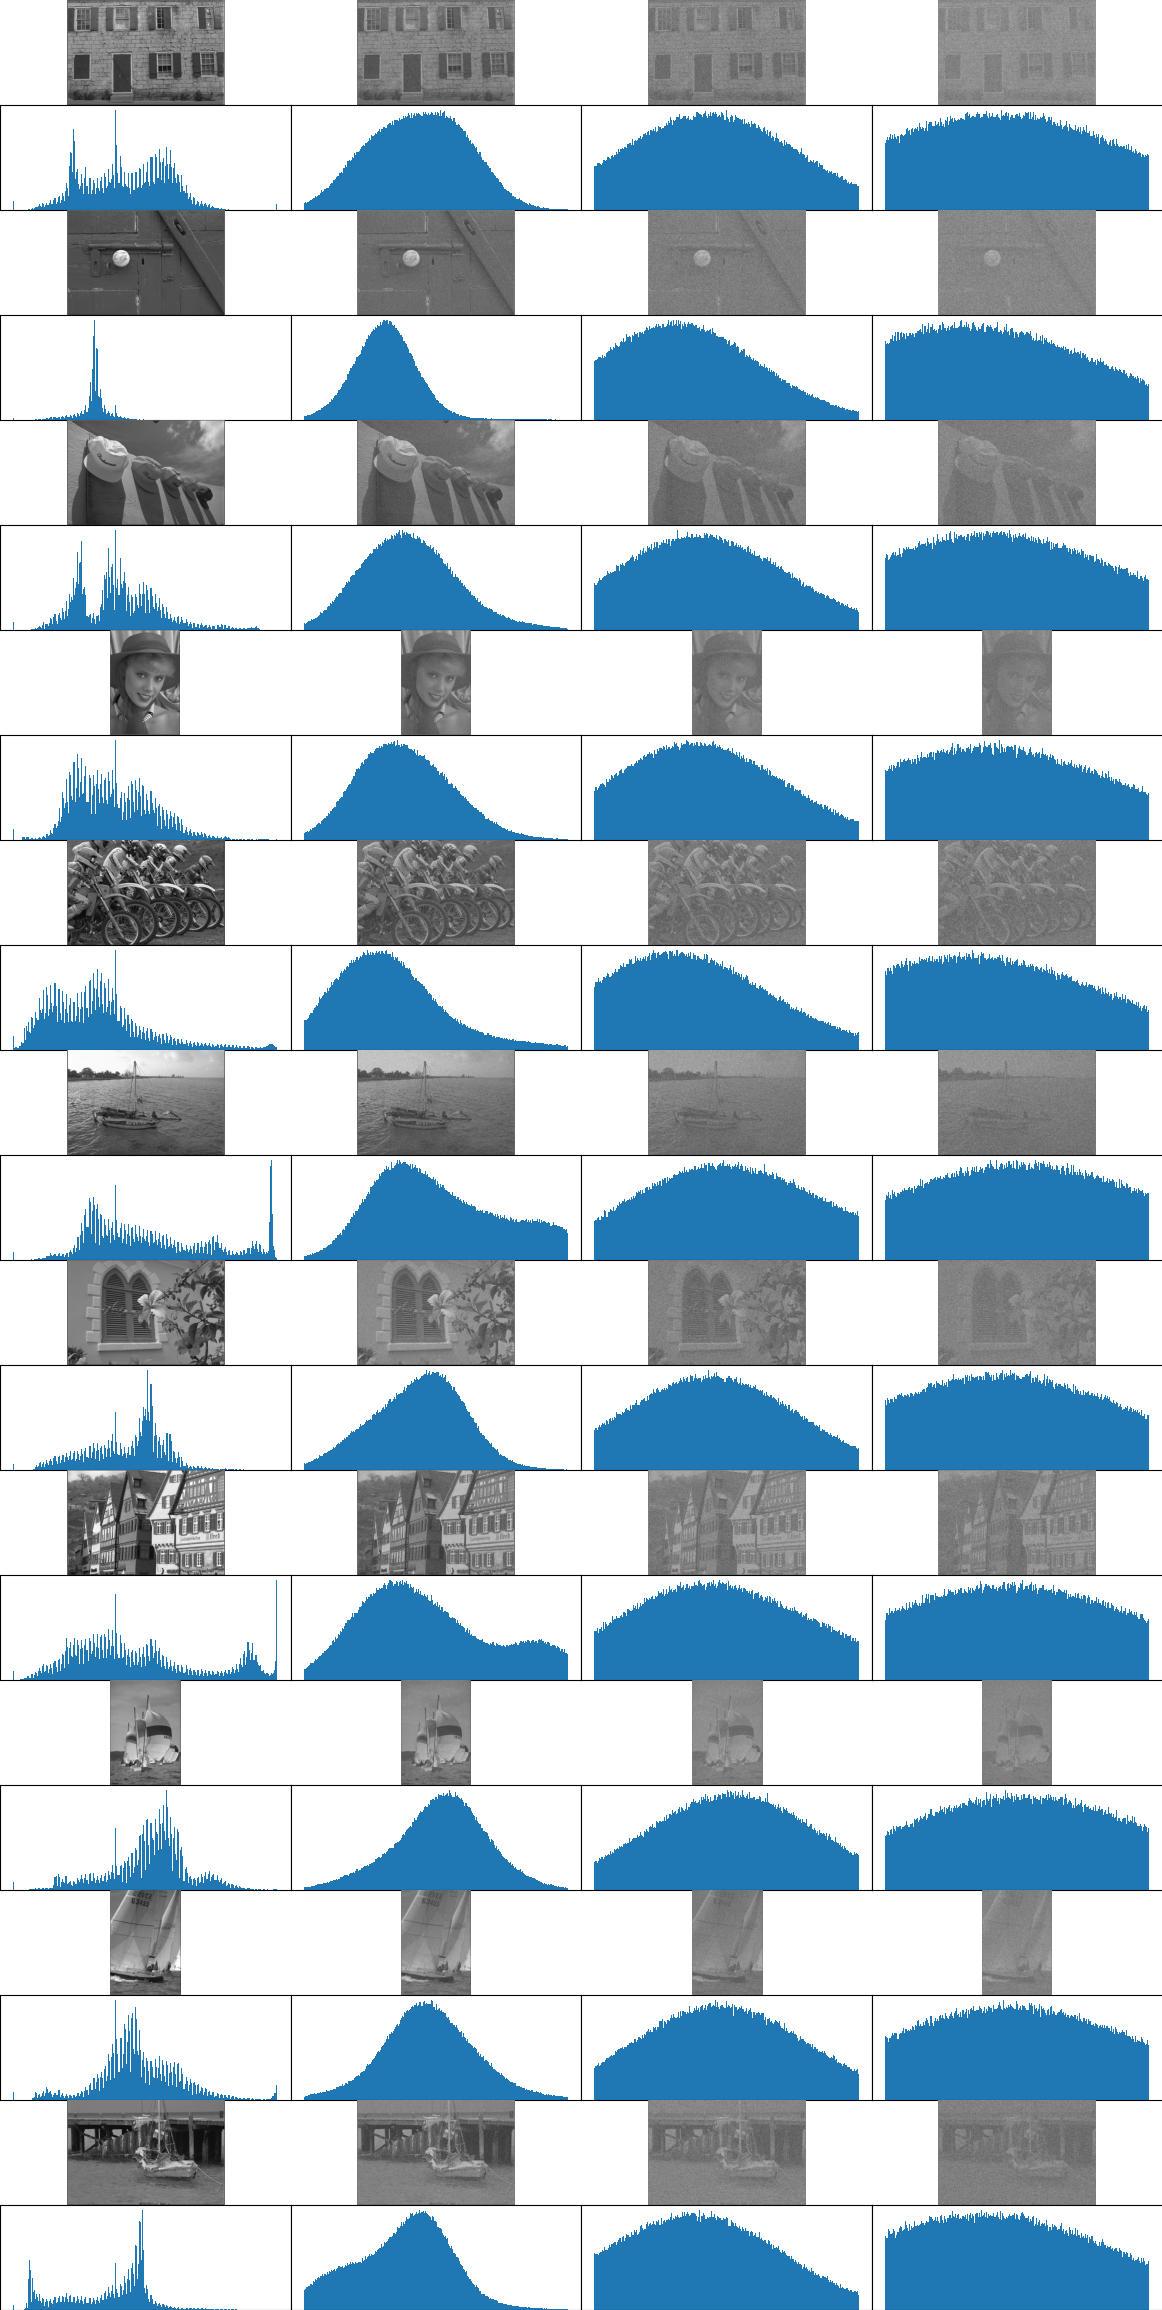
\includegraphics[width=\textwidth]{figuras/img_hist_noise_1.png}
    \caption{Imagen original junto con su histograma con distintos niveles de ruido, imagenes 1 a 5.}
\end{figure}


\begin{figure}
    \centering
    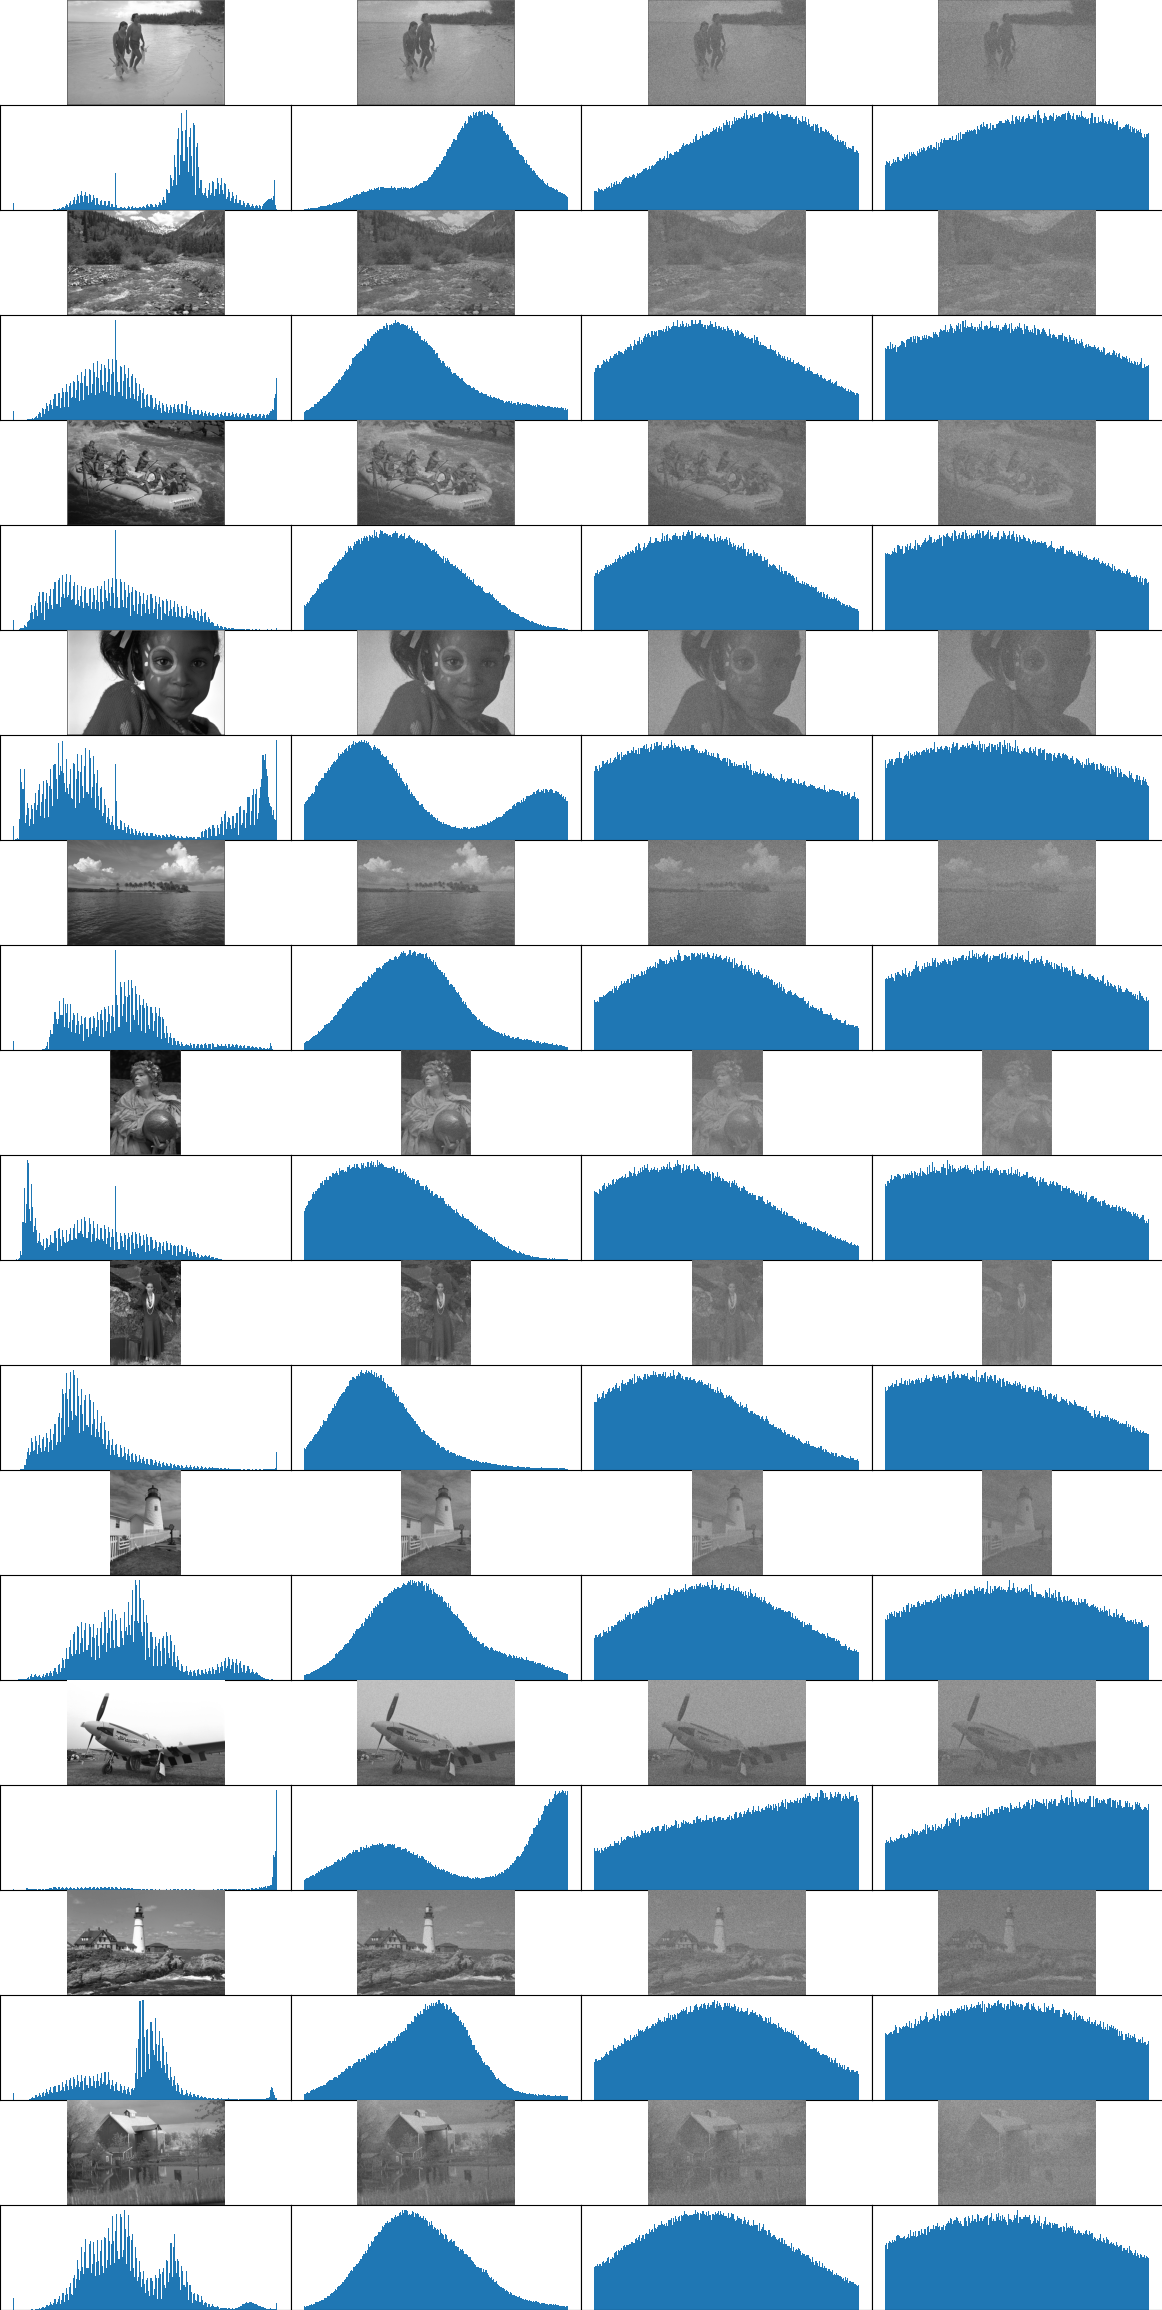
\includegraphics[width=\textwidth]{figuras/img_hist_noise_2.png}
    \caption{Imagen original junto con su histograma con distintos niveles de ruido, imagenes 6 a 10.}
\end{figure}


\begin{figure}
    \centering
    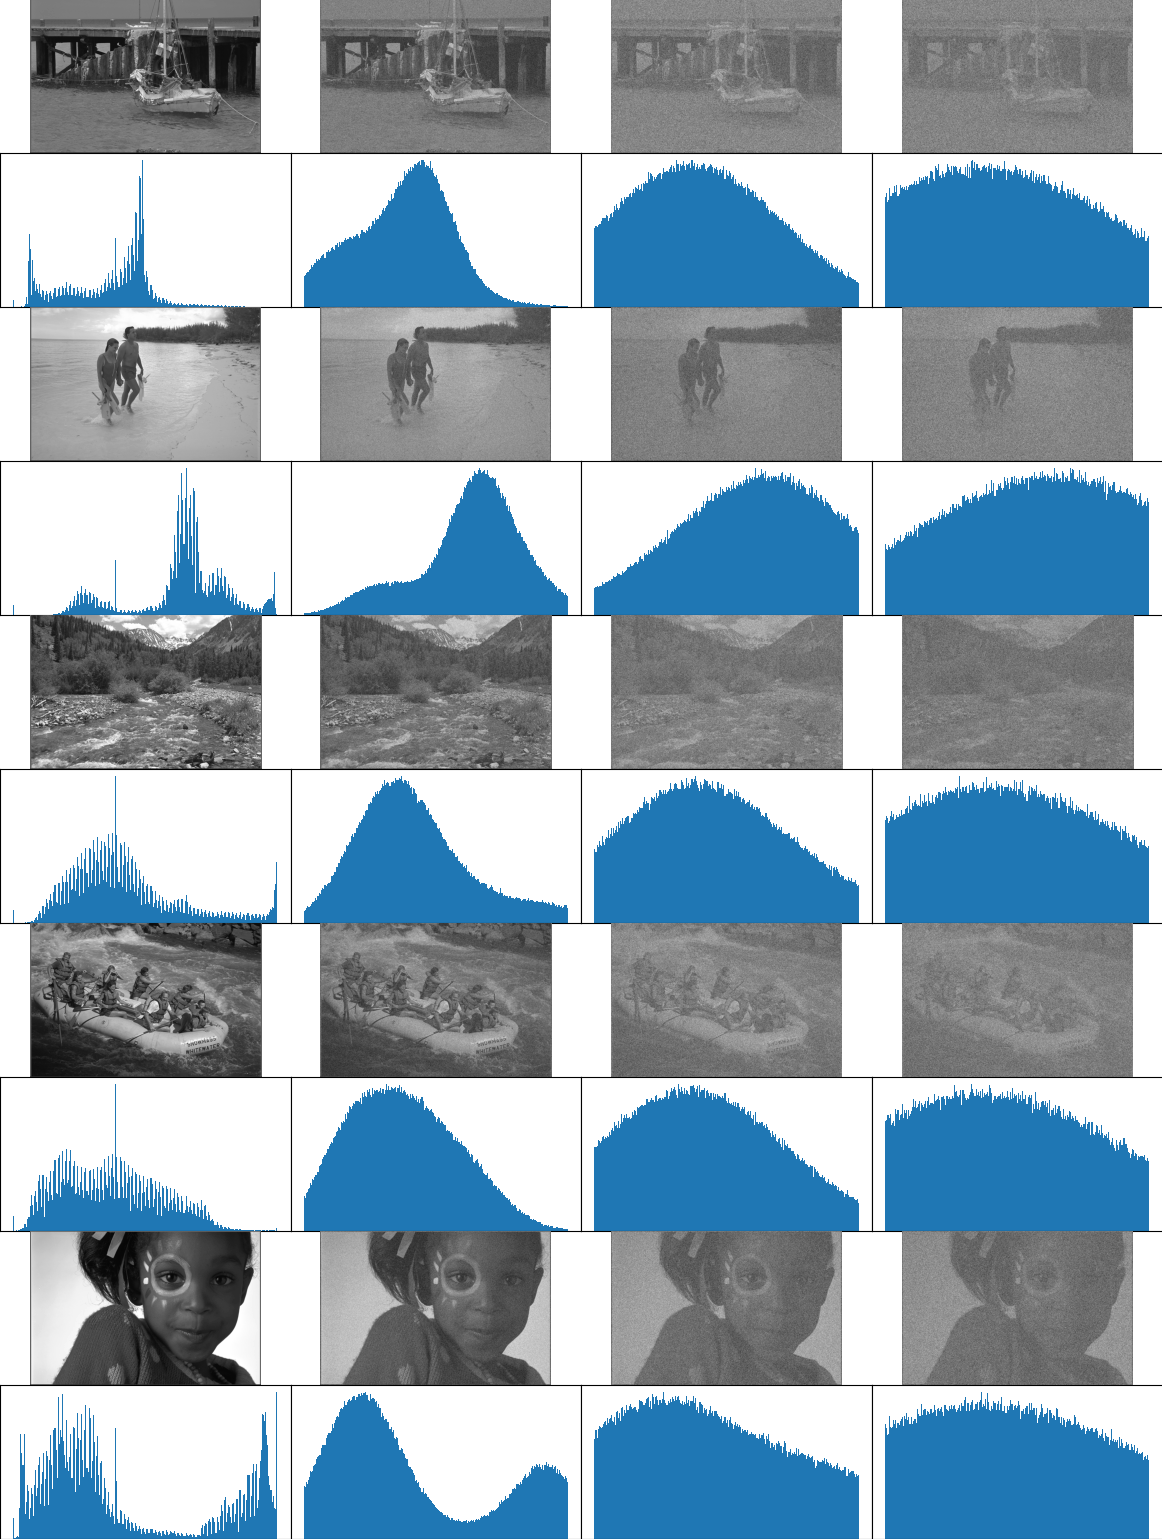
\includegraphics[width=\textwidth]{figuras/img_hist_noise_3.png}
    \caption{Imagen original junto con su histograma con distintos niveles de ruido, imagenes 11 a 15.}
\end{figure}


\begin{figure}
    \centering
    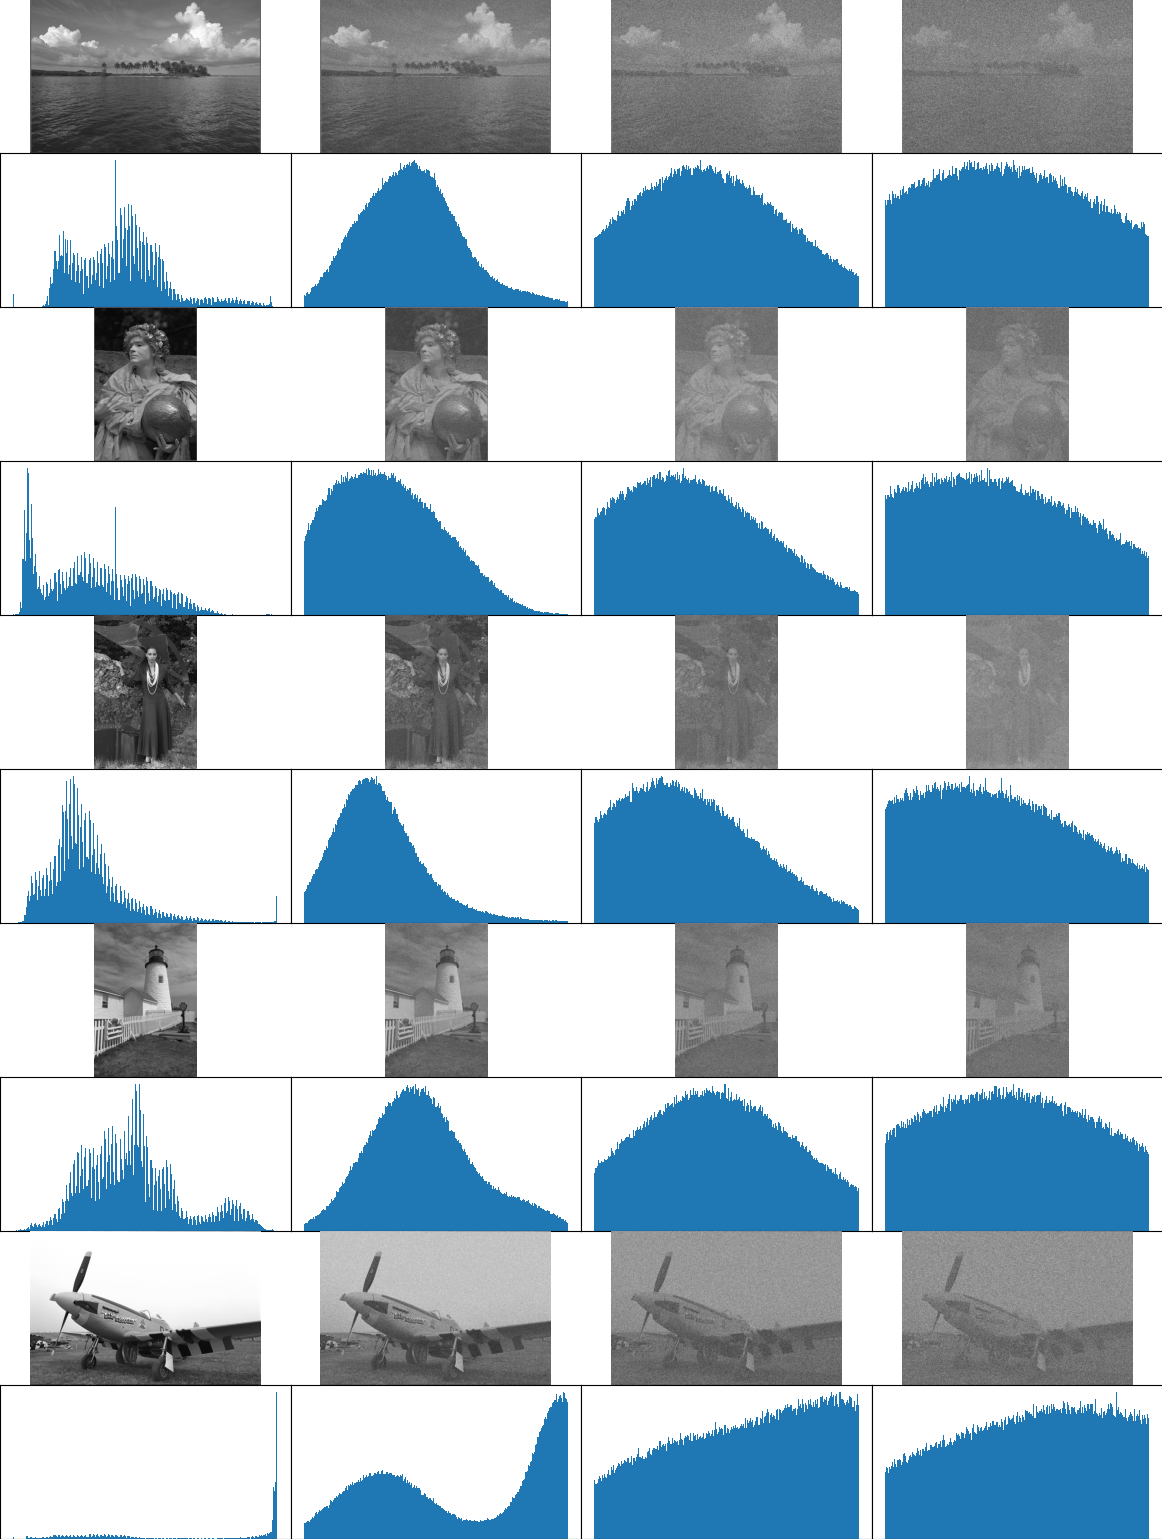
\includegraphics[width=\textwidth]{figuras/img_hist_noise_4.png}
    \caption{Imagen original junto con su histograma con distintos niveles de ruido, imagenes 16 a 20.}
\end{figure}


\begin{figure}
    \centering
    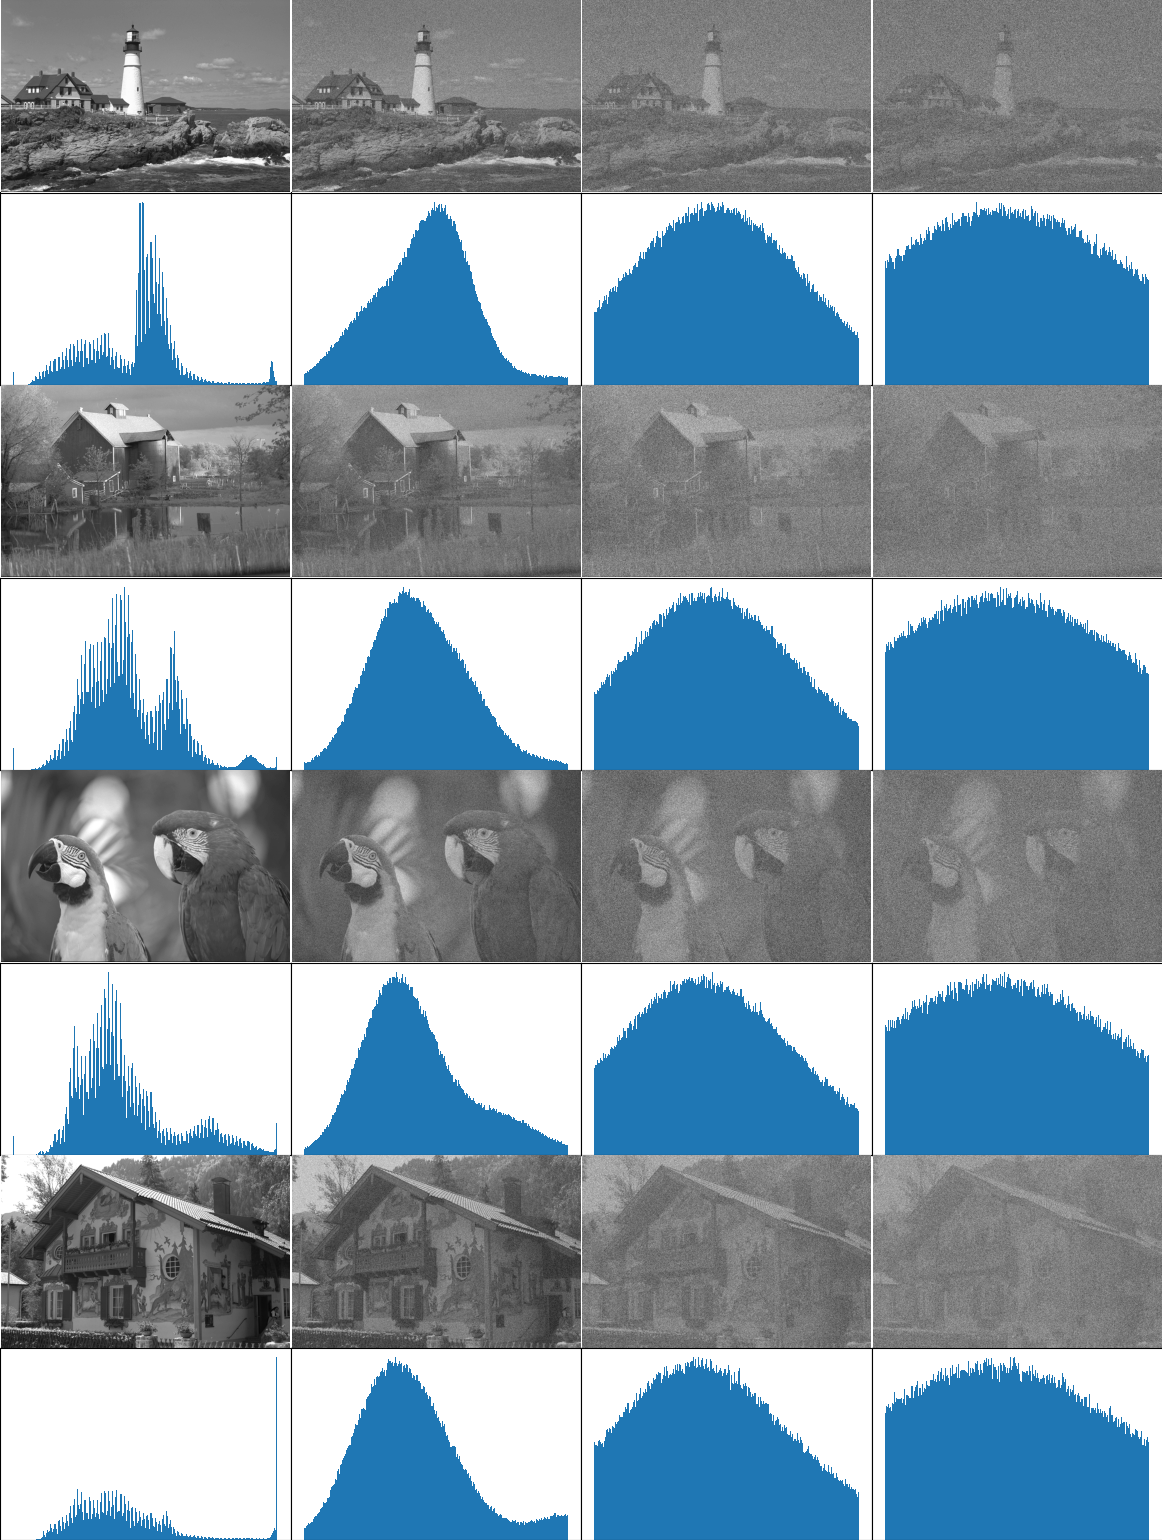
\includegraphics[width=\textwidth]{figuras/img_hist_noise_5.png}
    \caption{Imagen original junto con su histograma con distintos niveles de ruido, imagenes 21 a 25.}
\end{figure}

\begin{figure}
    \centering
    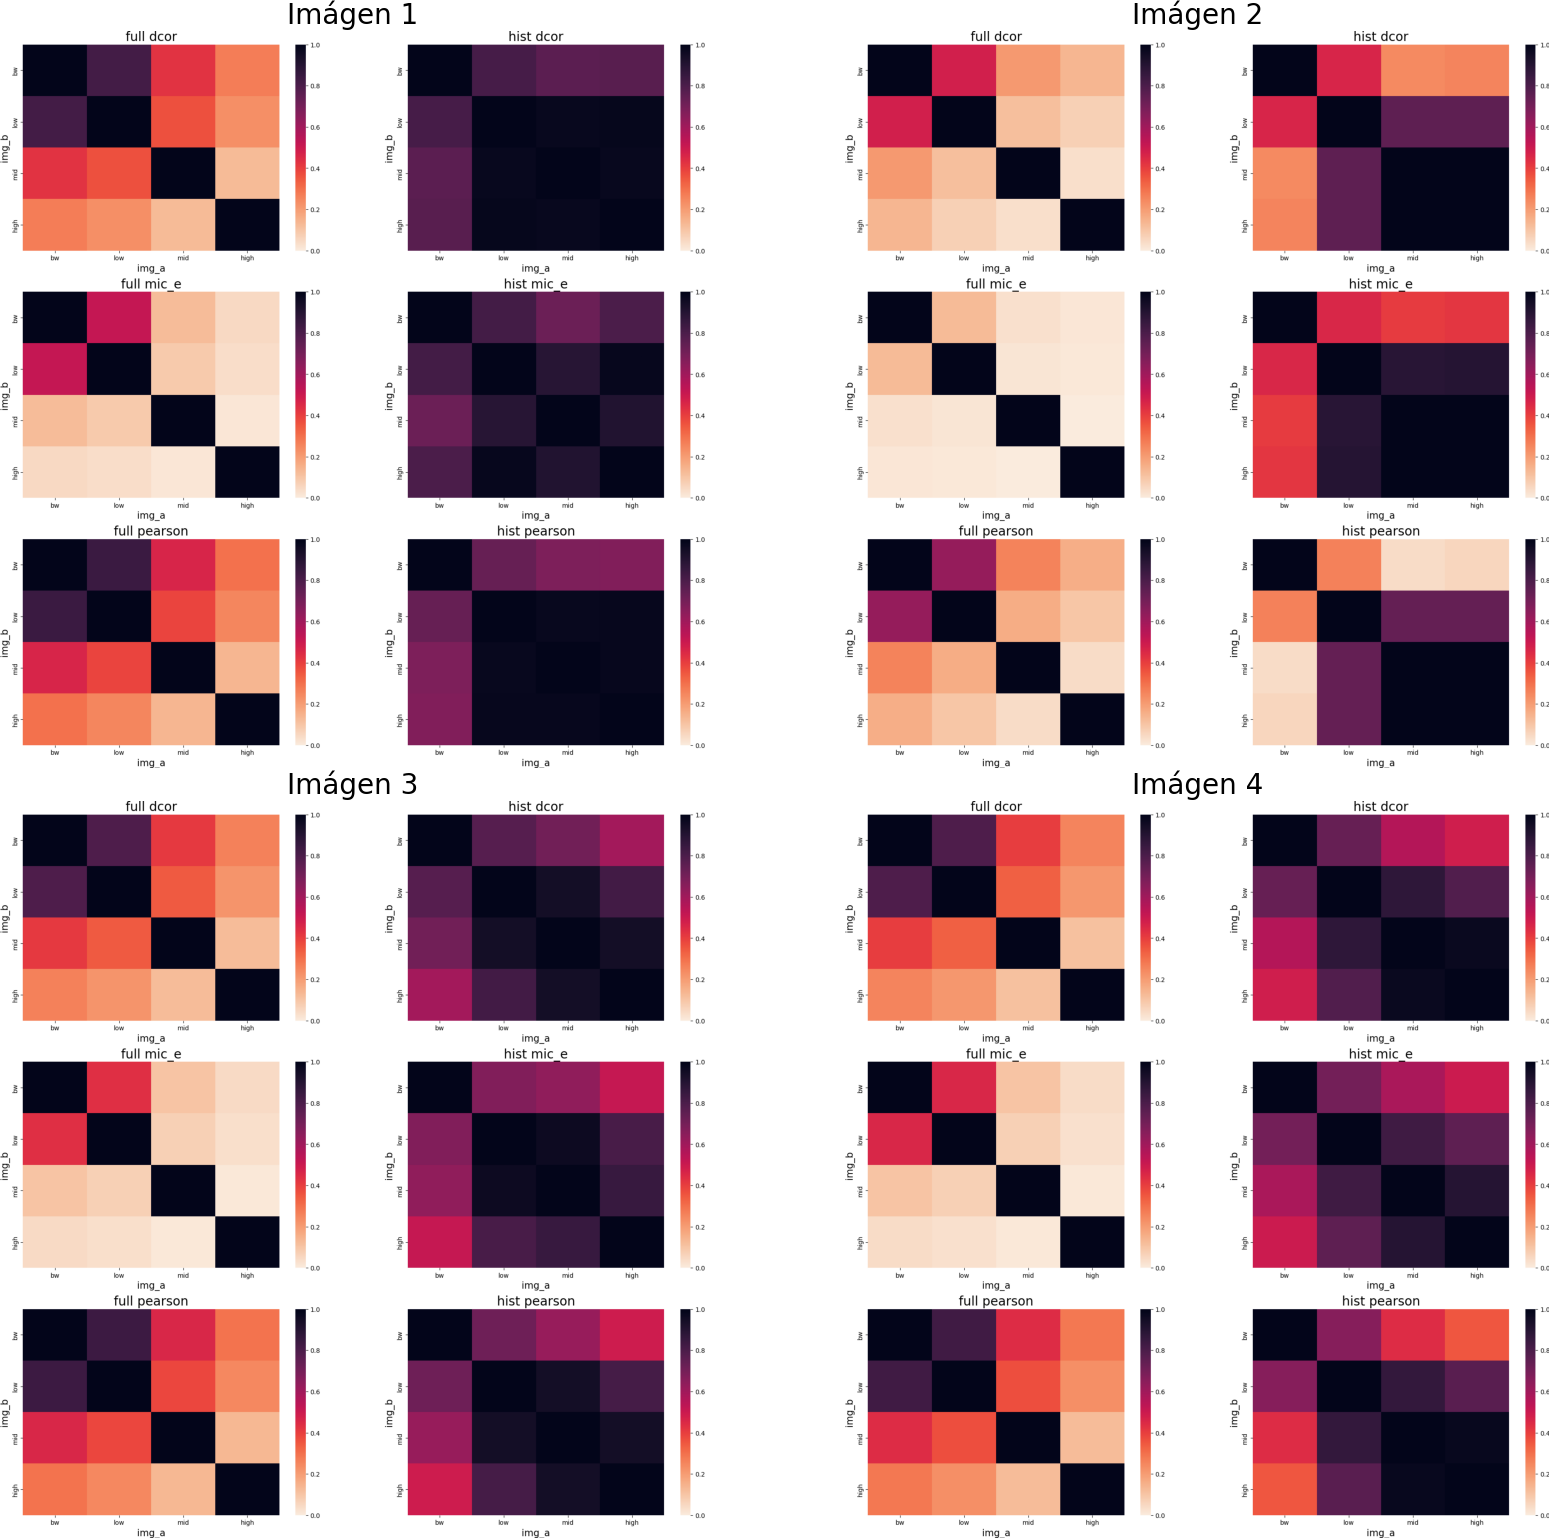
\includegraphics[width=\textwidth]{figuras/heatmaps/heatmaps_app_0.png}
    \caption{Matriz de calor para las imagenes 1, 2, 3, y 4, cada mapa de calor corresponde a un m\'etodo de comparaci\'on, ya sea comparando el total de la im\'agen (izquierda), o el histograma de estas (derecha). La cantidad de ruido aumenta de izquierda a derecha, y de arriba hacía abajo.}
\end{figure}

\begin{figure}
    \centering
    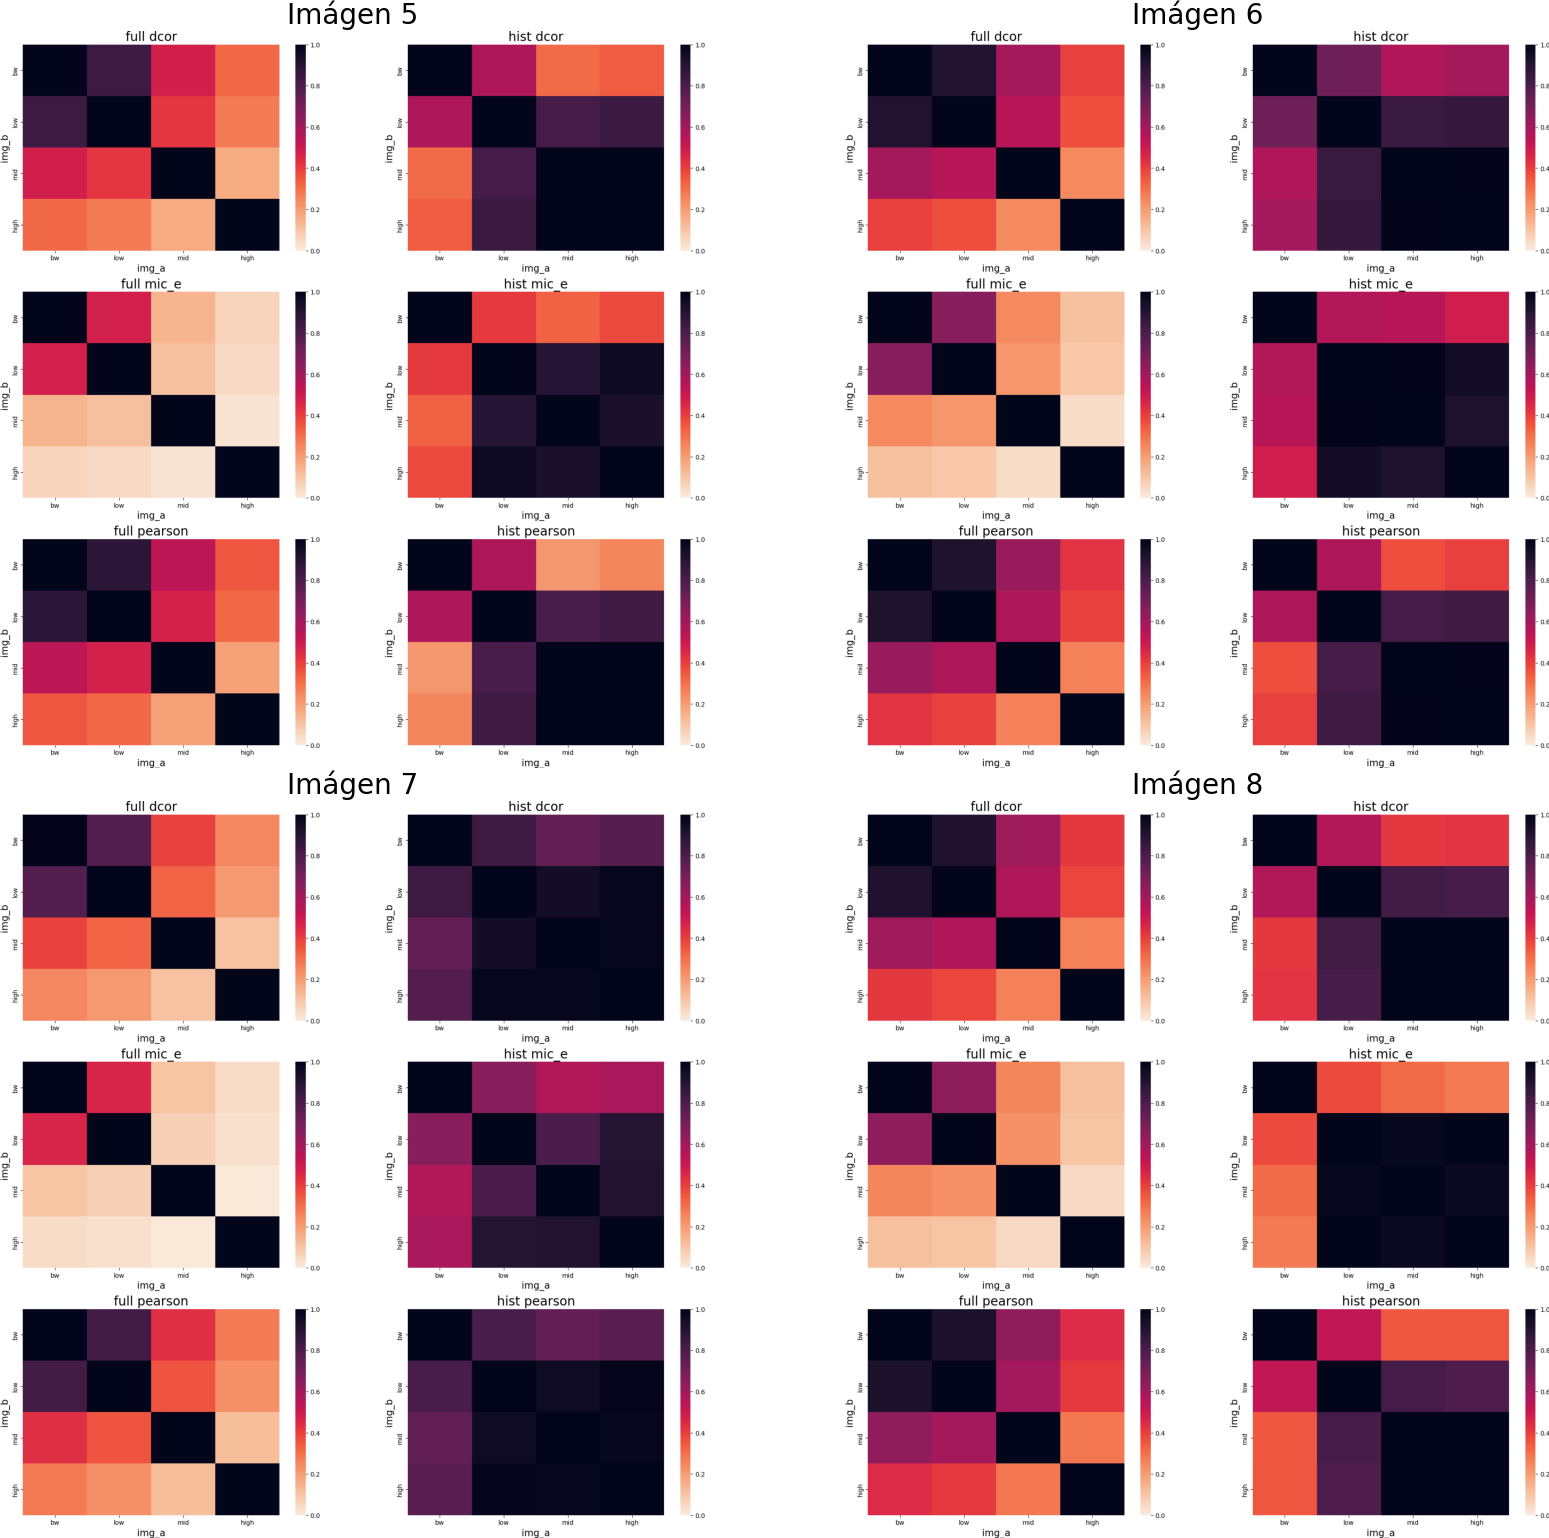
\includegraphics[width=\textwidth]{figuras/heatmaps/heatmaps_app_1.png}
    \caption{Matriz de calor para las imagenes 5, 6, 7, y 8, cada mapa de calor corresponde a un m\'etodo de comparaci\'on, ya sea comparando el total de la im\'agen (izquierda), o el histograma de estas (derecha). La cantidad de ruido aumenta de izquierda a derecha, y de arriba hacía abajo.}
\end{figure}


\begin{figure}
    \centering
    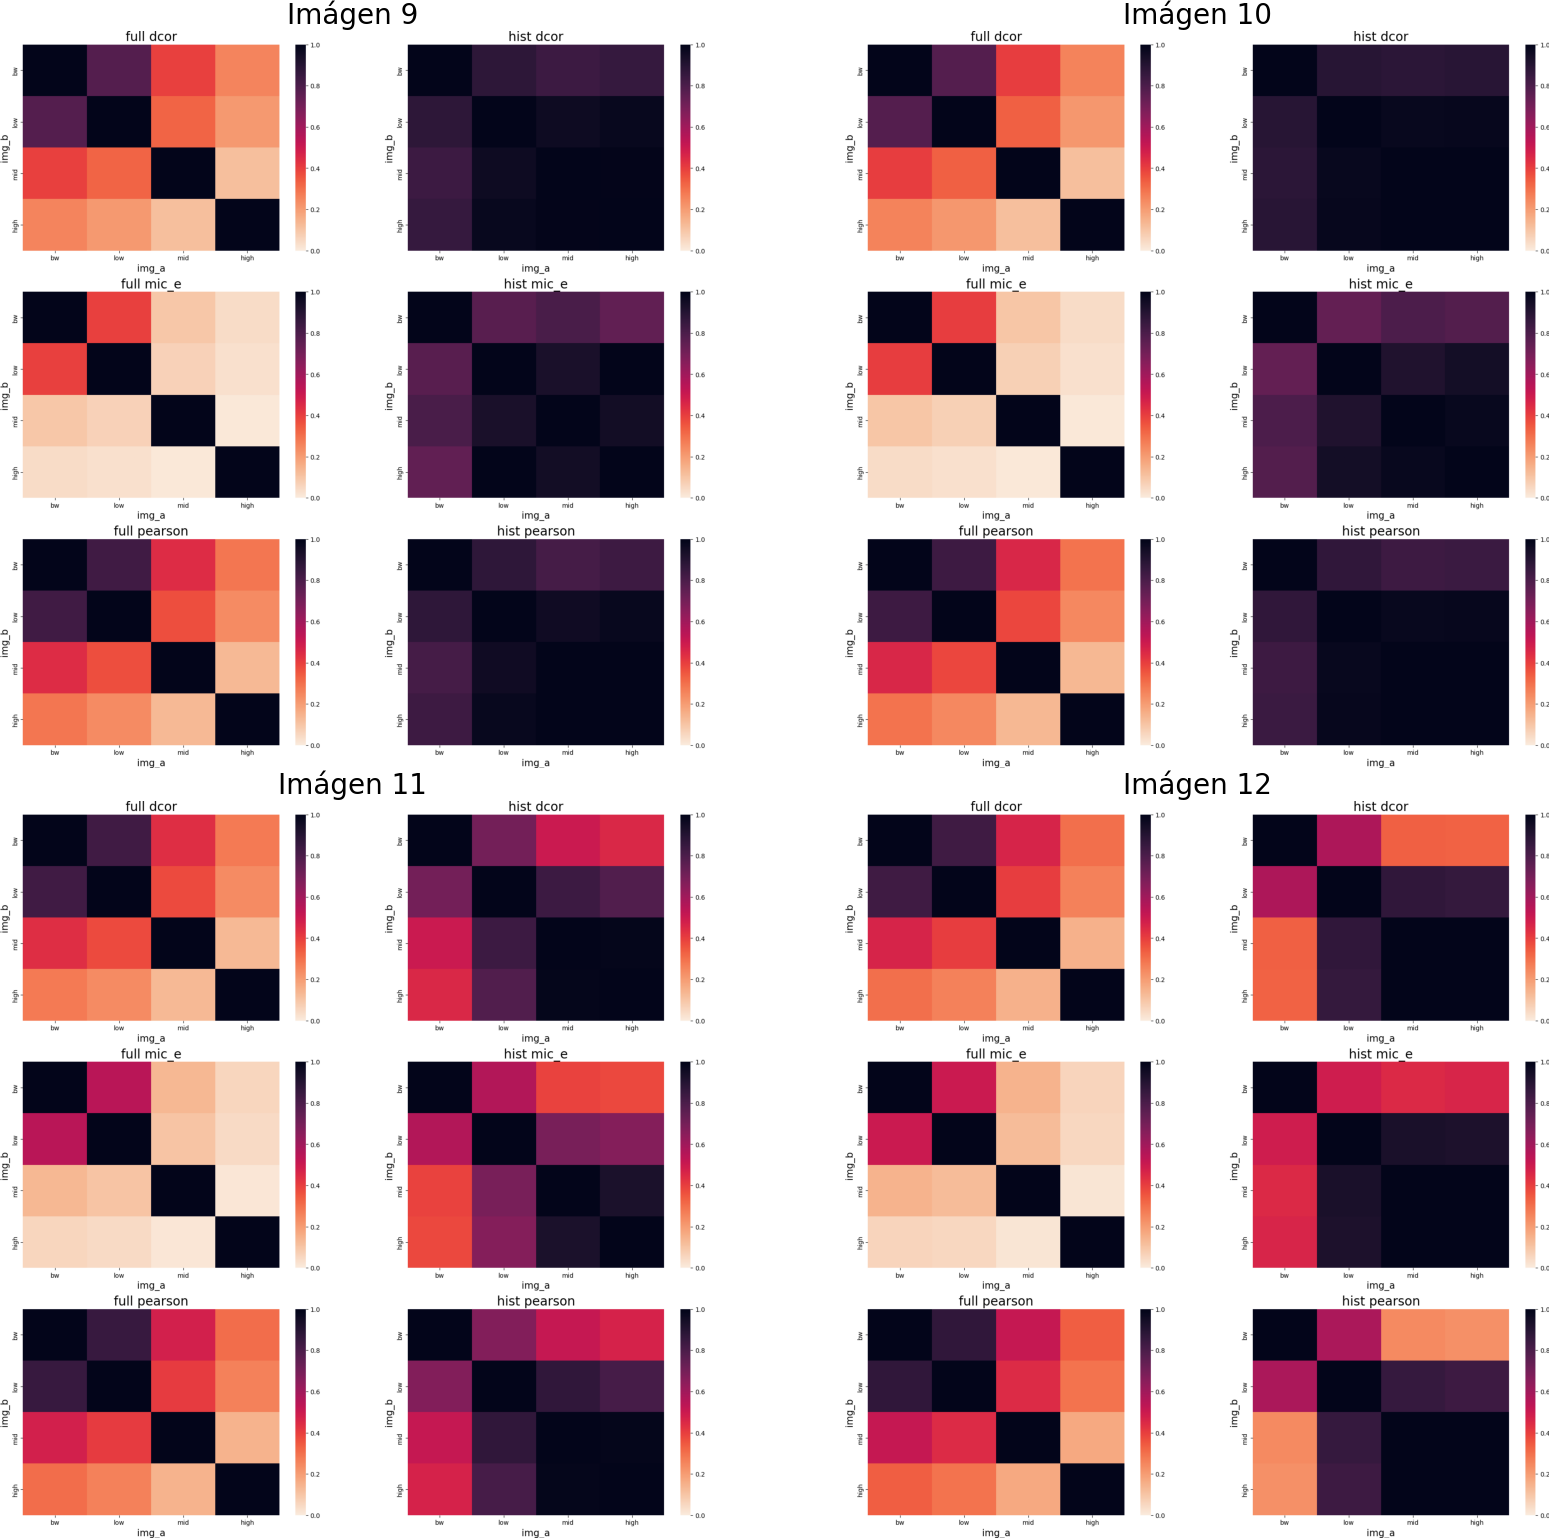
\includegraphics[width=\textwidth]{figuras/heatmaps/heatmaps_app_2.png}
    \caption{Matriz de calor para las imagenes 9, 10, 11, y 12, cada mapa de calor corresponde a un m\'etodo de comparaci\'on, ya sea comparando el total de la im\'agen (izquierda), o el histograma de estas (derecha). La cantidad de ruido aumenta de izquierda a derecha, y de arriba hacía abajo.}
\end{figure}


\begin{figure}
    \centering
    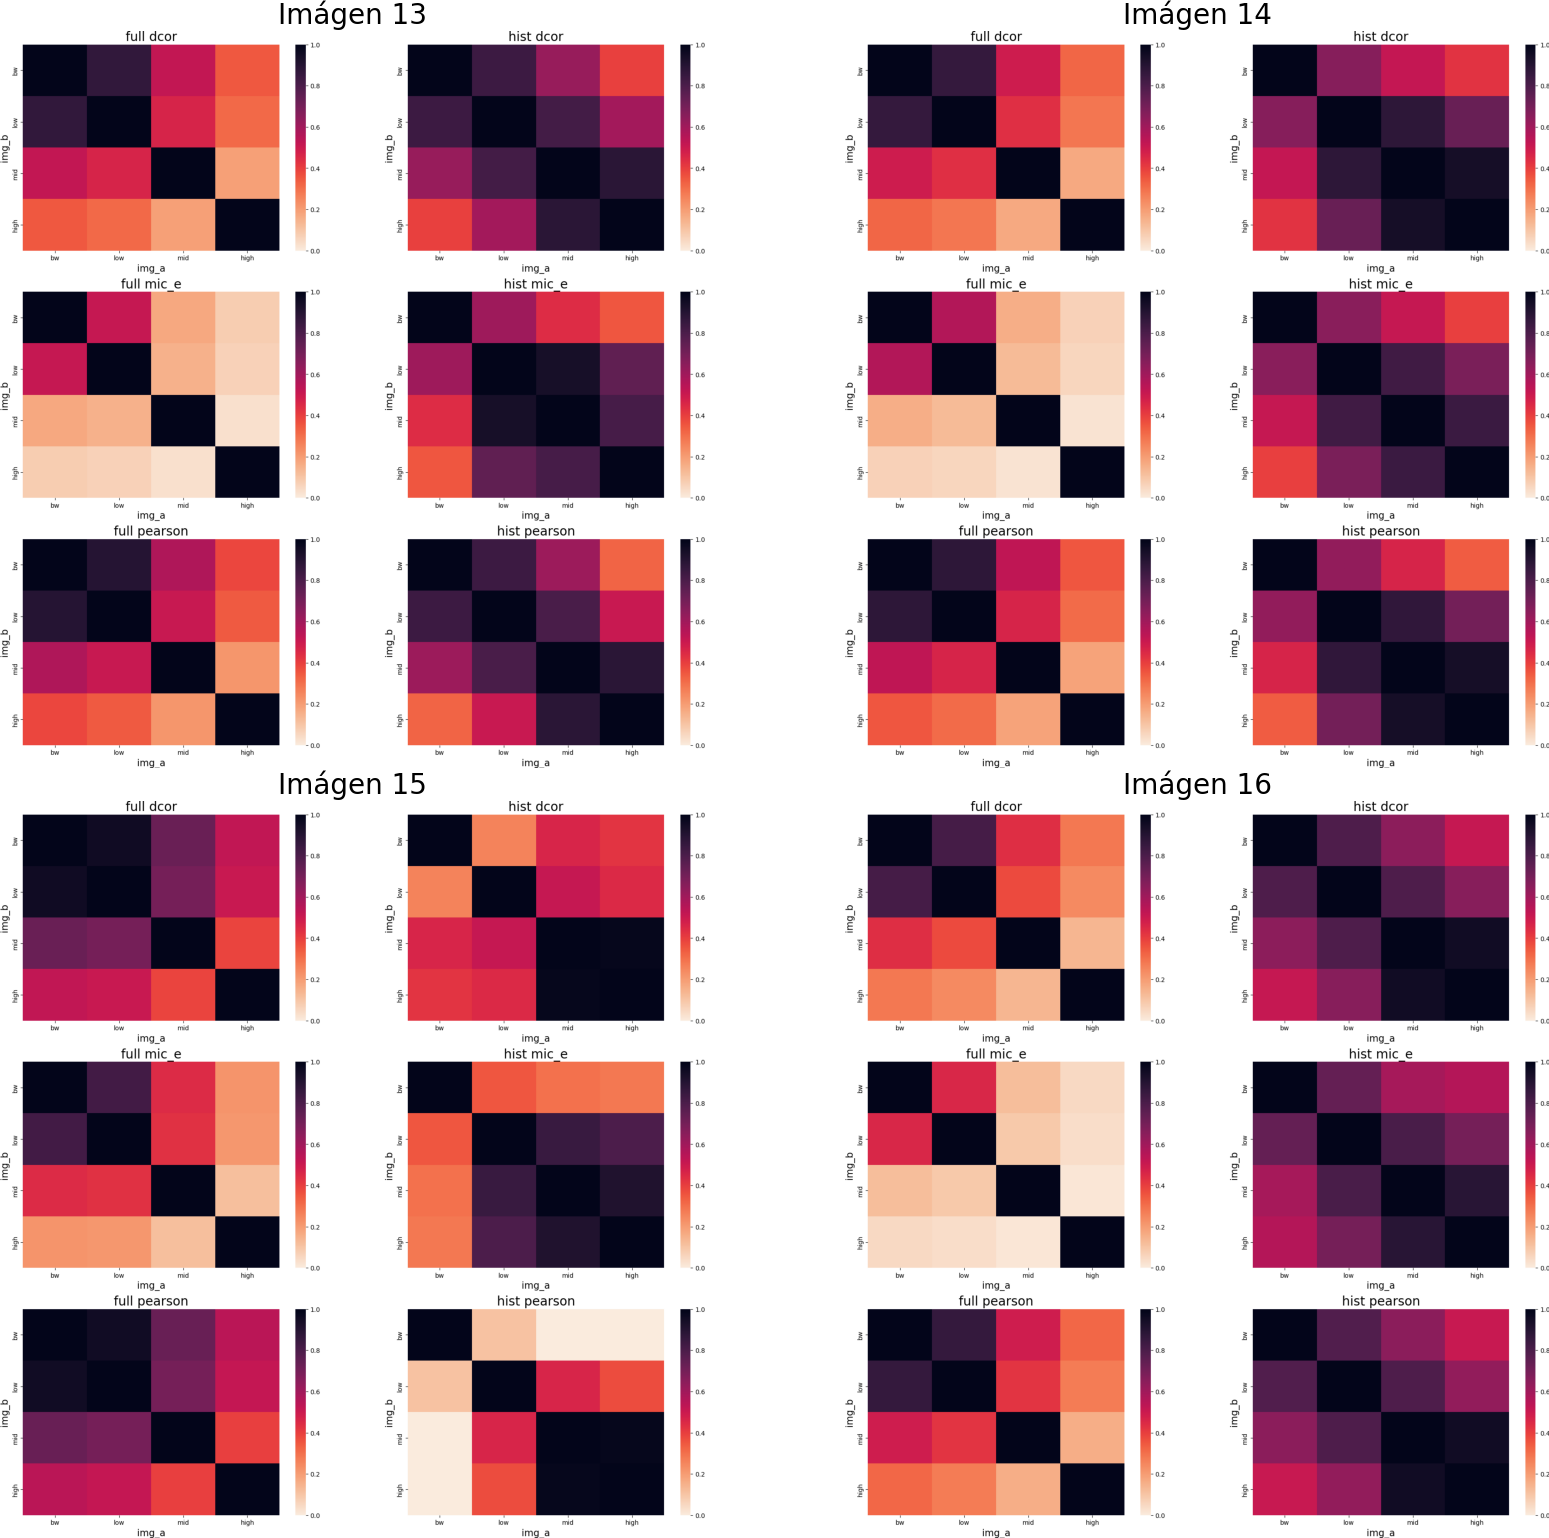
\includegraphics[width=\textwidth]{figuras/heatmaps/heatmaps_app_3.png}
    \caption{Matriz de calor para las imagenes 13, 14, 15, y 16, cada mapa de calor corresponde a un m\'etodo de comparaci\'on, ya sea comparando el total de la im\'agen (izquierda), o el histograma de estas (derecha). La cantidad de ruido aumenta de izquierda a derecha, y de arriba hacía abajo.}
\end{figure}


\begin{figure}
    \centering
    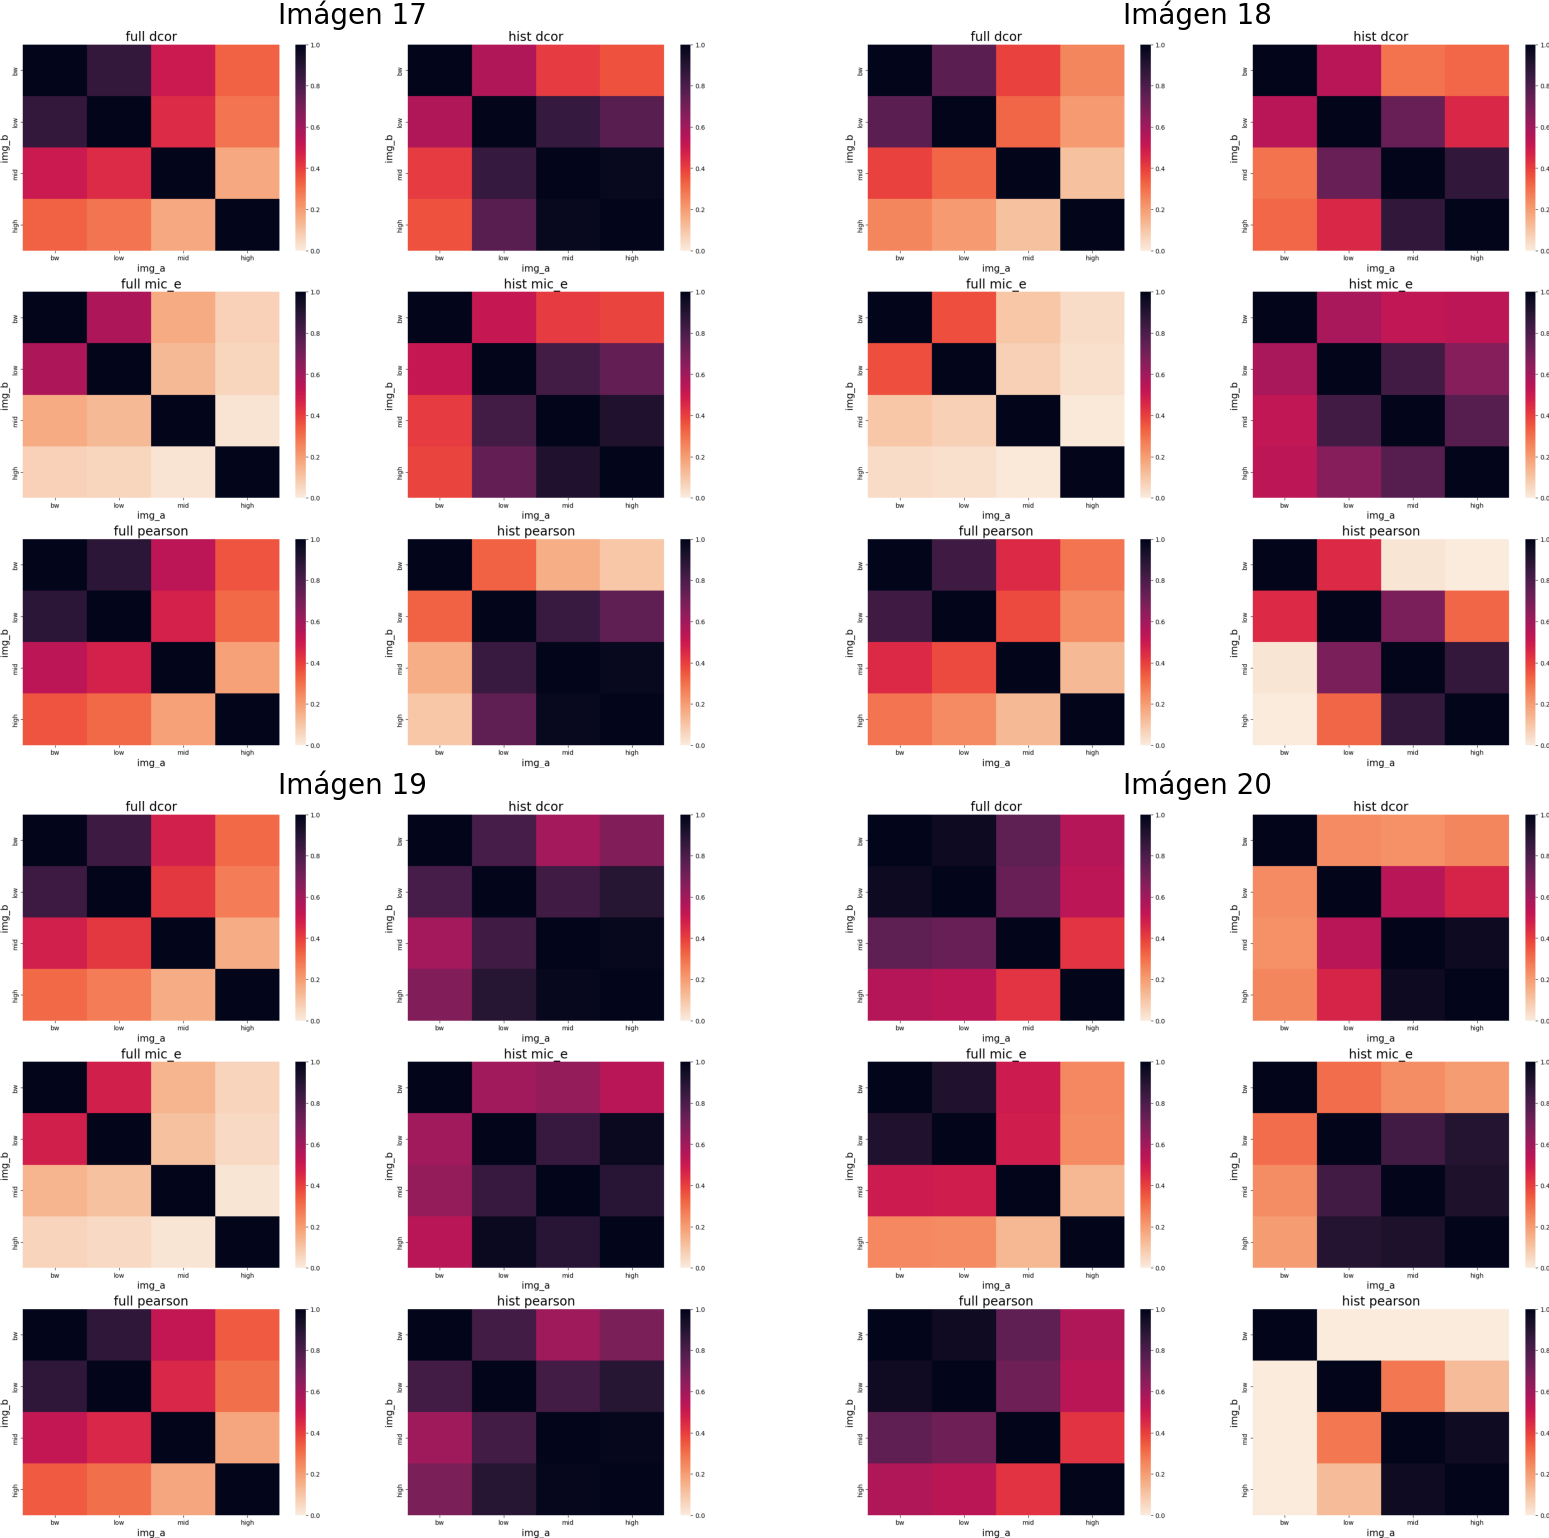
\includegraphics[width=\textwidth]{figuras/heatmaps/heatmaps_app_4.png}
    \caption{Matriz de calor para las imagenes 17, 18, 19, y 20, cada mapa de calor corresponde a un m\'etodo de comparaci\'on, ya sea comparando el total de la im\'agen (izquierda), o el histograma de estas (derecha). La cantidad de ruido aumenta de izquierda a derecha, y de arriba hacía abajo.}
\end{figure}


\begin{figure}
    \centering
    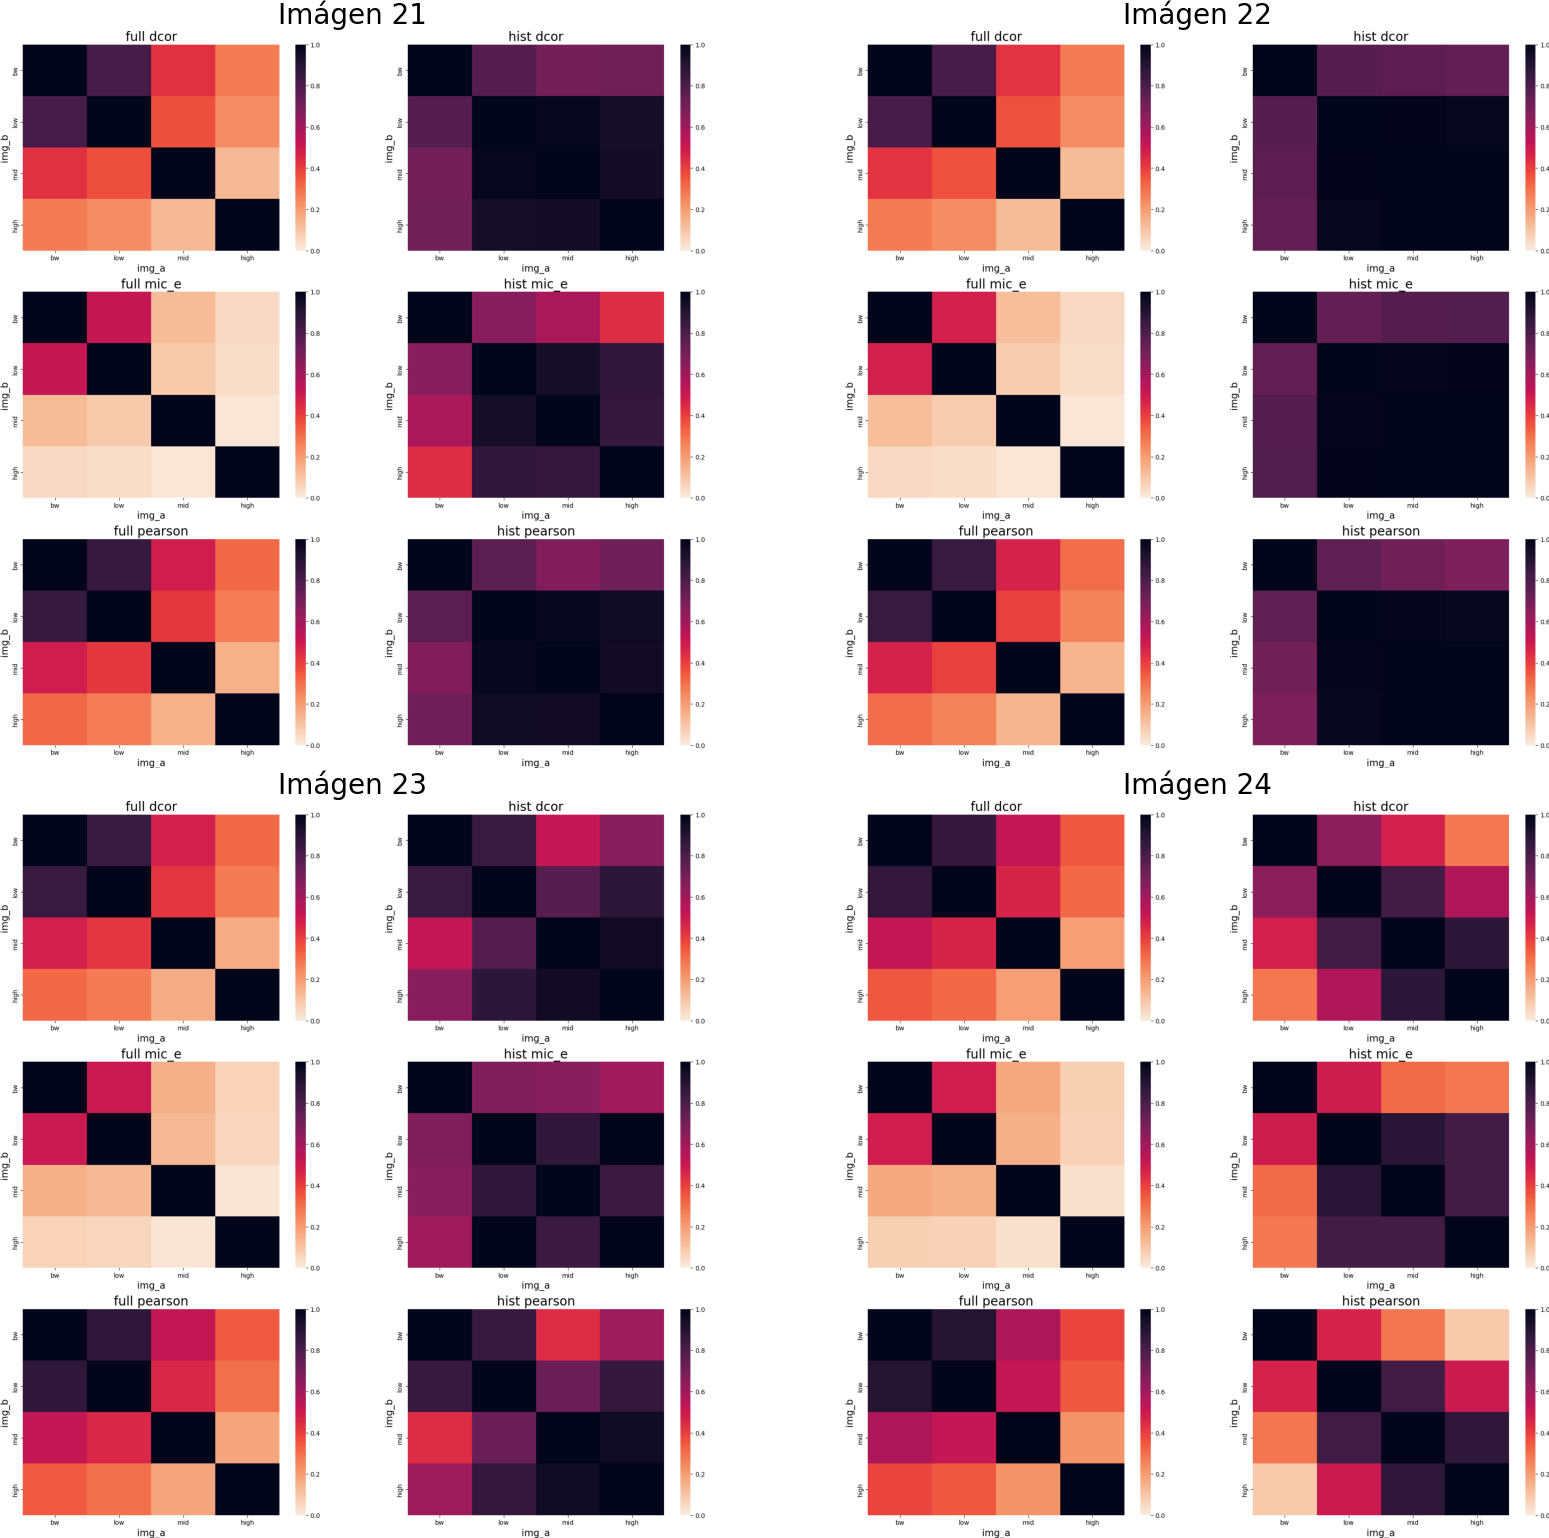
\includegraphics[width=\textwidth]{figuras/heatmaps/heatmaps_app_5.png}
    \caption{Matriz de calor para las imagenes 21, 22, 23, y 24, cada mapa de calor corresponde a un m\'etodo de comparaci\'on, ya sea comparando el total de la im\'agen (izquierda), o el histograma de estas (derecha). La cantidad de ruido aumenta de izquierda a derecha, y de arriba hacía abajo.}
\end{figure}



\begin{figure}
    \centering
    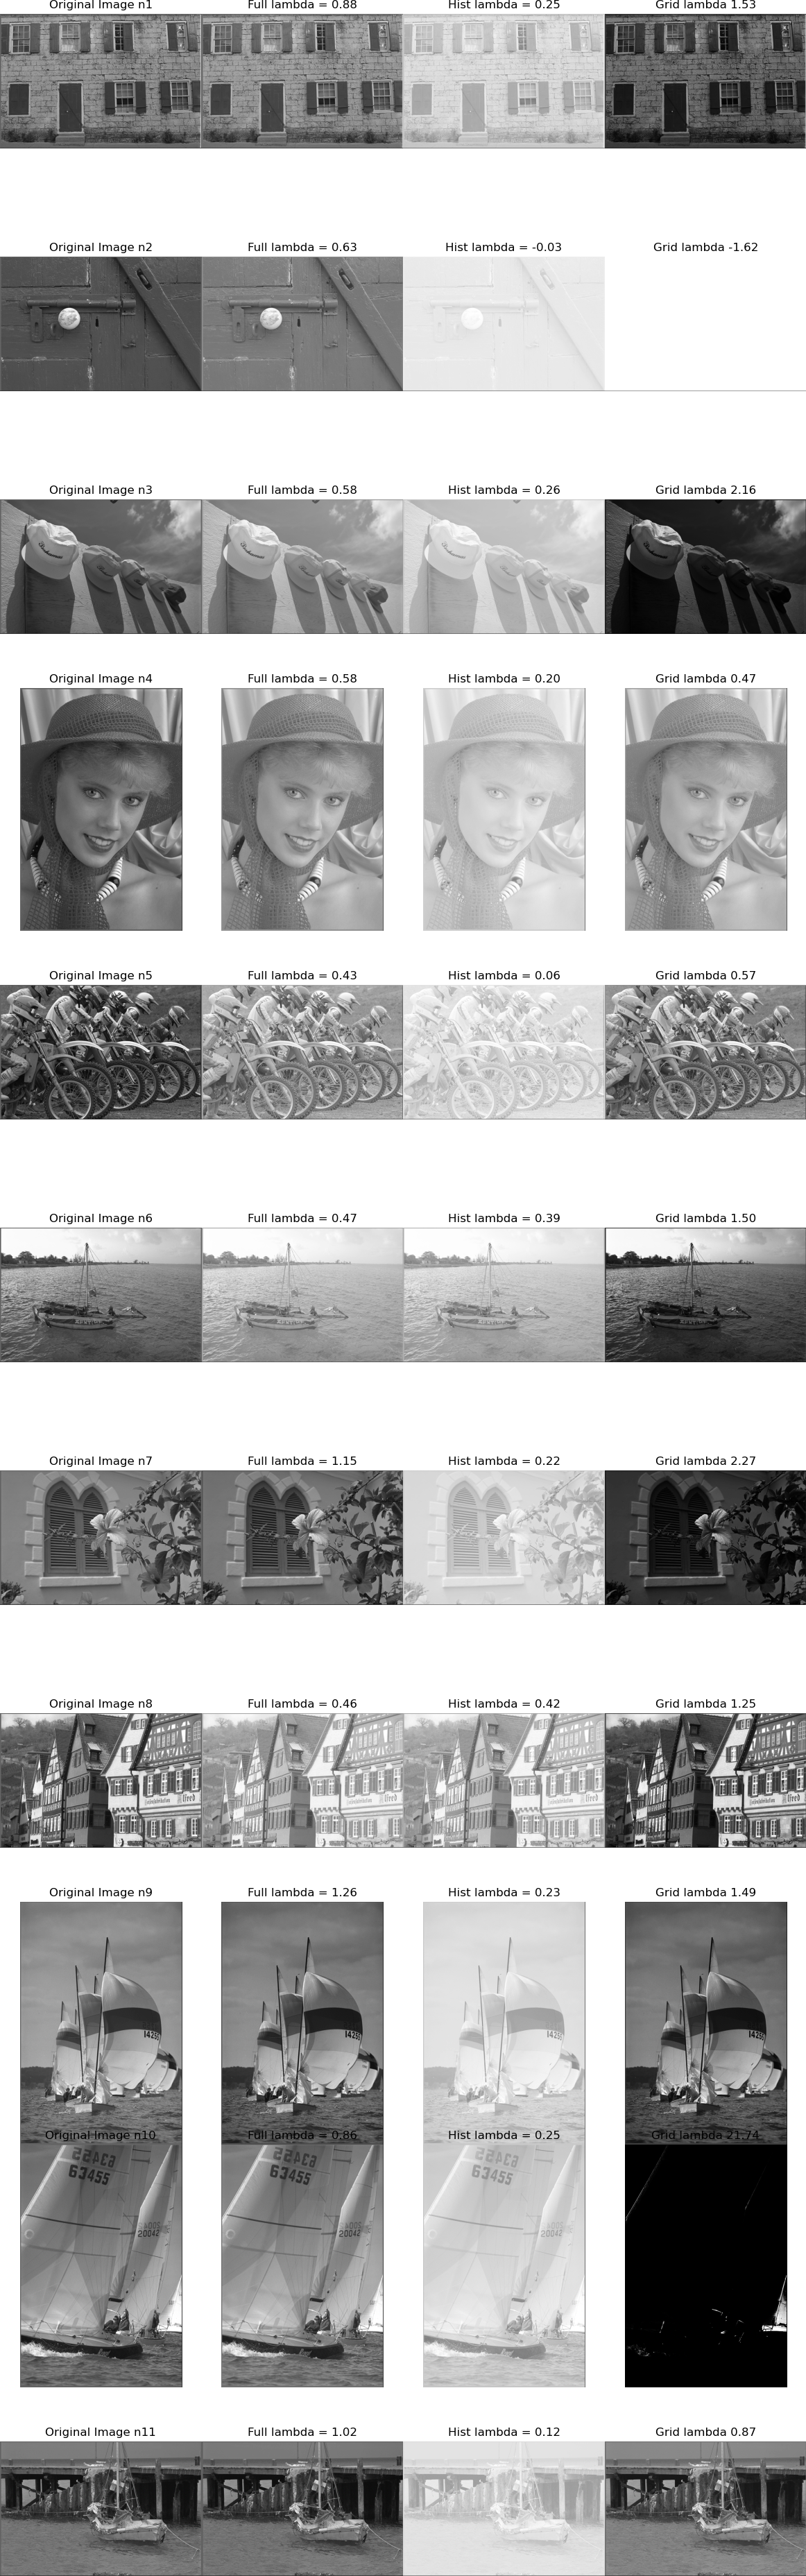
\includegraphics[width=\textwidth]{figuras/img_BCI_all_1.png}
    \caption{Imagen original junto con sus transformaci\'ones Box-Cox para los distintos m\'etodos de $\lambda$transformados, primera las im\'agenes 1 a 5.}
\end{figure}

\begin{figure}
    \centering
    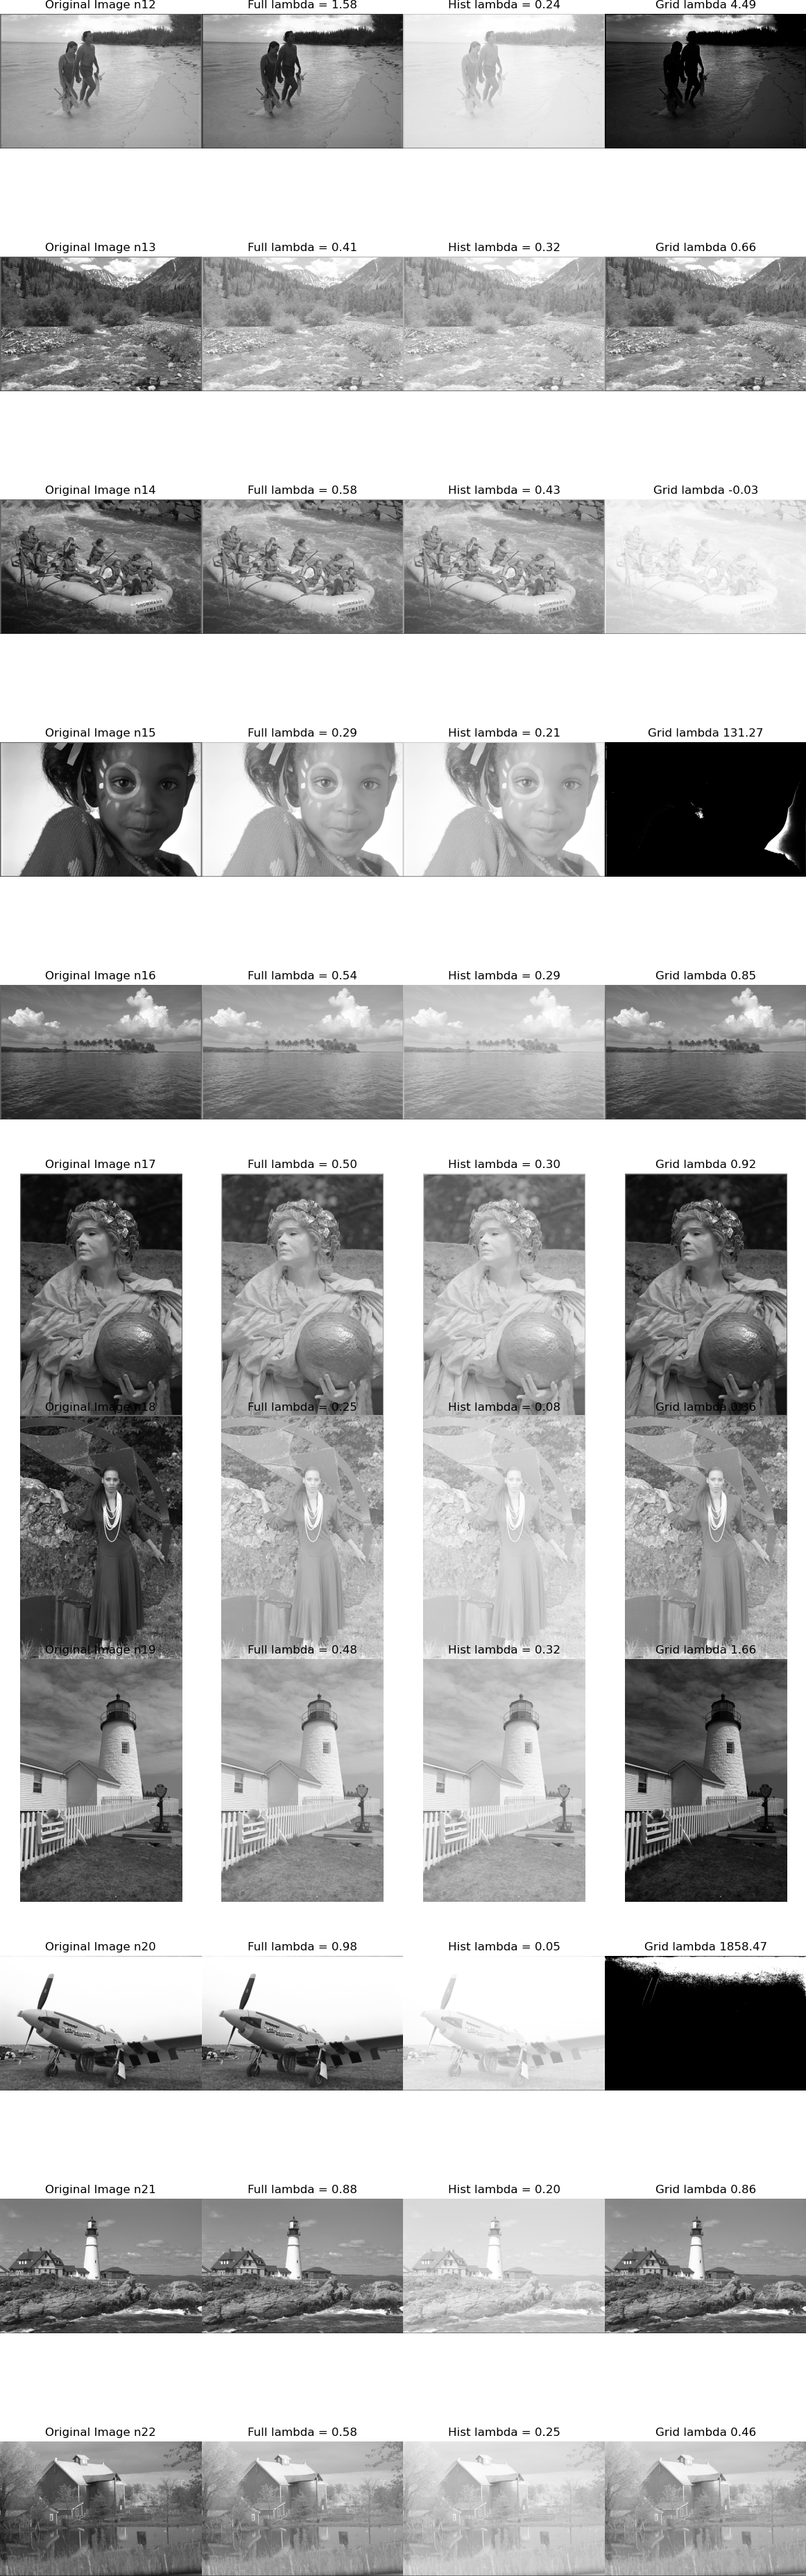
\includegraphics[width=\textwidth]{figuras/img_BCI_all_2.png}
    \caption{Imagen original junto con sus transformaci\'ones Box-Cox para los distintos m\'etodos de $\lambda$transformados, primera las im\'agenes 6 a 12.}
\end{figure}


\begin{figure}
    \centering
    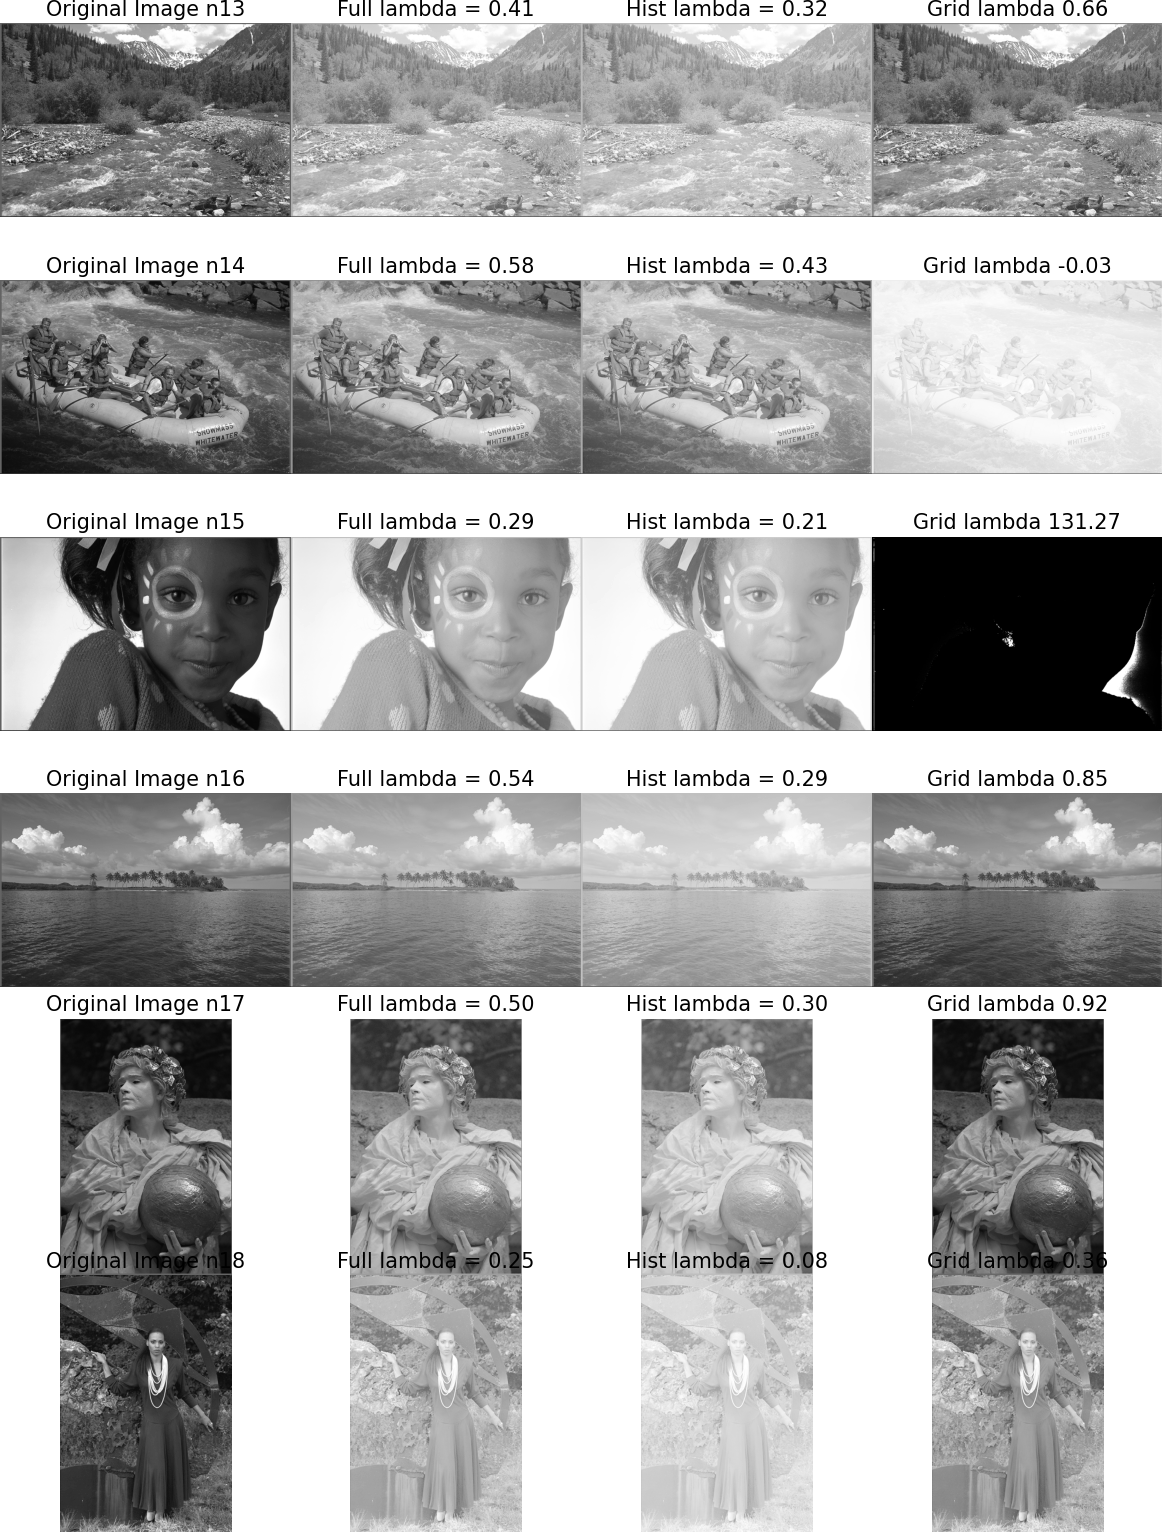
\includegraphics[width=\textwidth]{figuras/img_BCI_all_3.png}
    \caption{Imagen original junto con sus transformaci\'ones Box-Cox para los distintos m\'etodos de $\lambda$transformados, primera las im\'agenes 13 a 18.}
\end{figure}


\begin{figure}
    \centering
    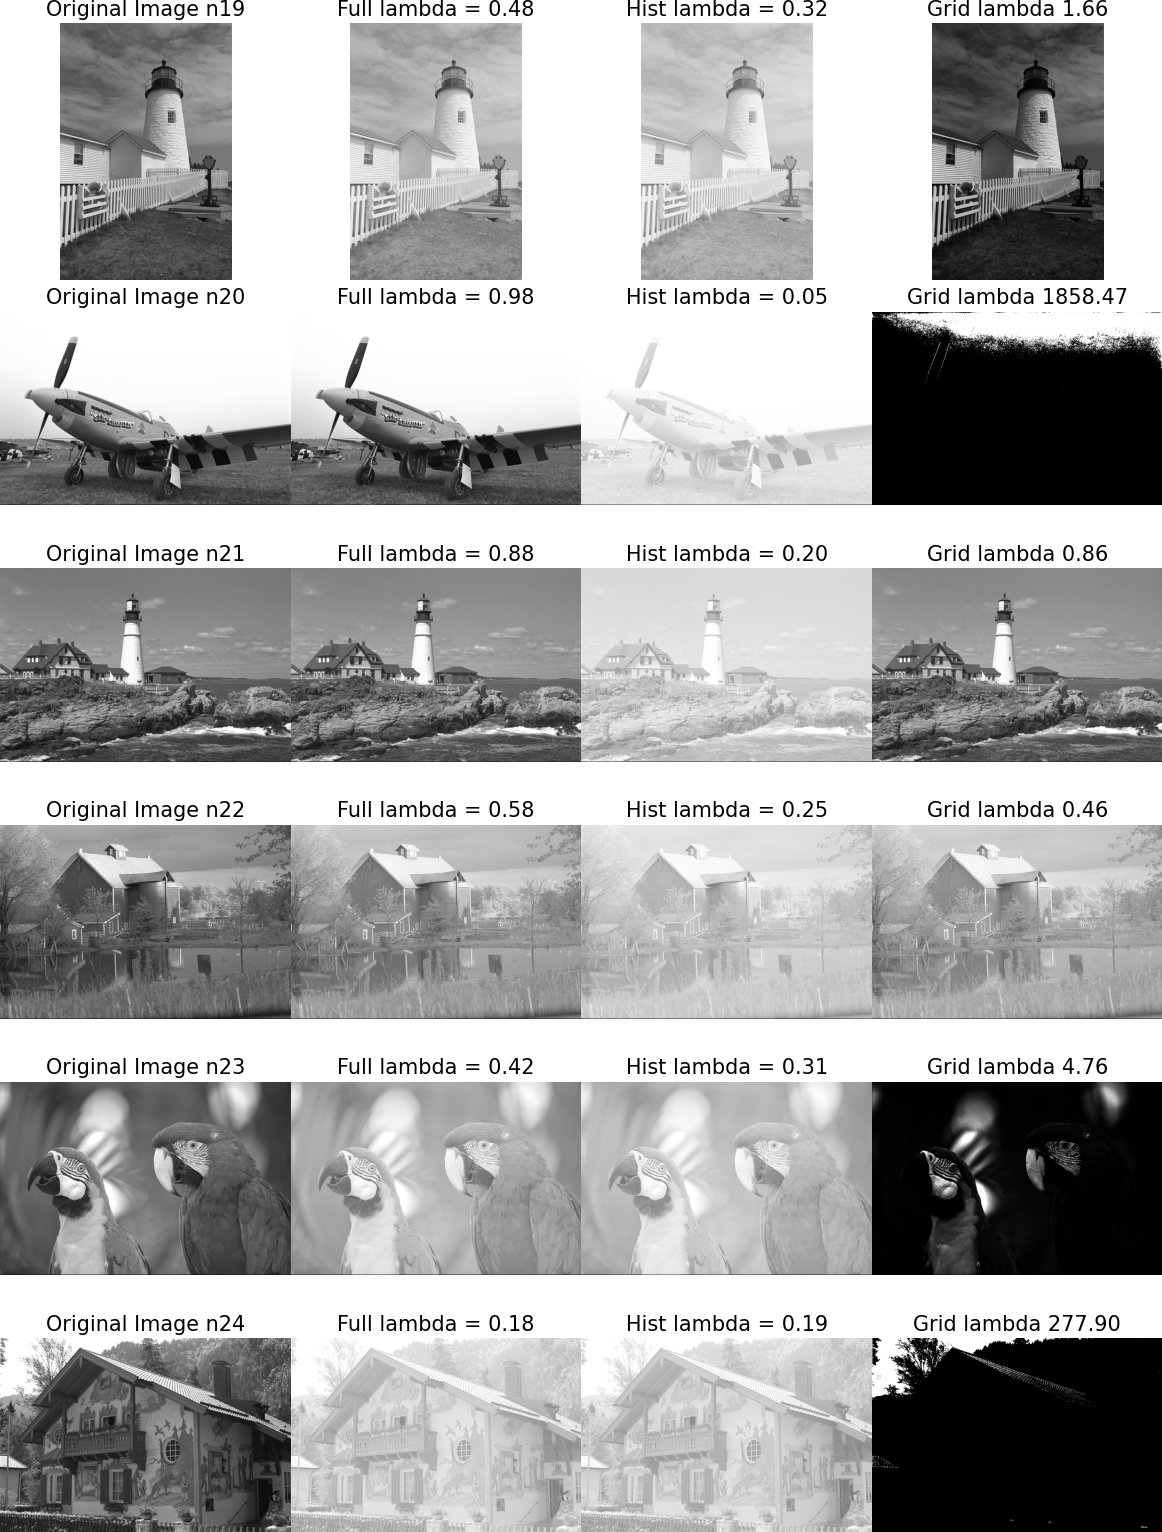
\includegraphics[width=\textwidth]{figuras/img_BCI_all_4.png}
    \caption{Imagen original junto con sus transformaci\'ones Box-Cox para los distintos m\'etodos de $\lambda$transformados, primera las im\'agenes 19 a 24.}
\end{figure}


\begin{figure}
    \centering
    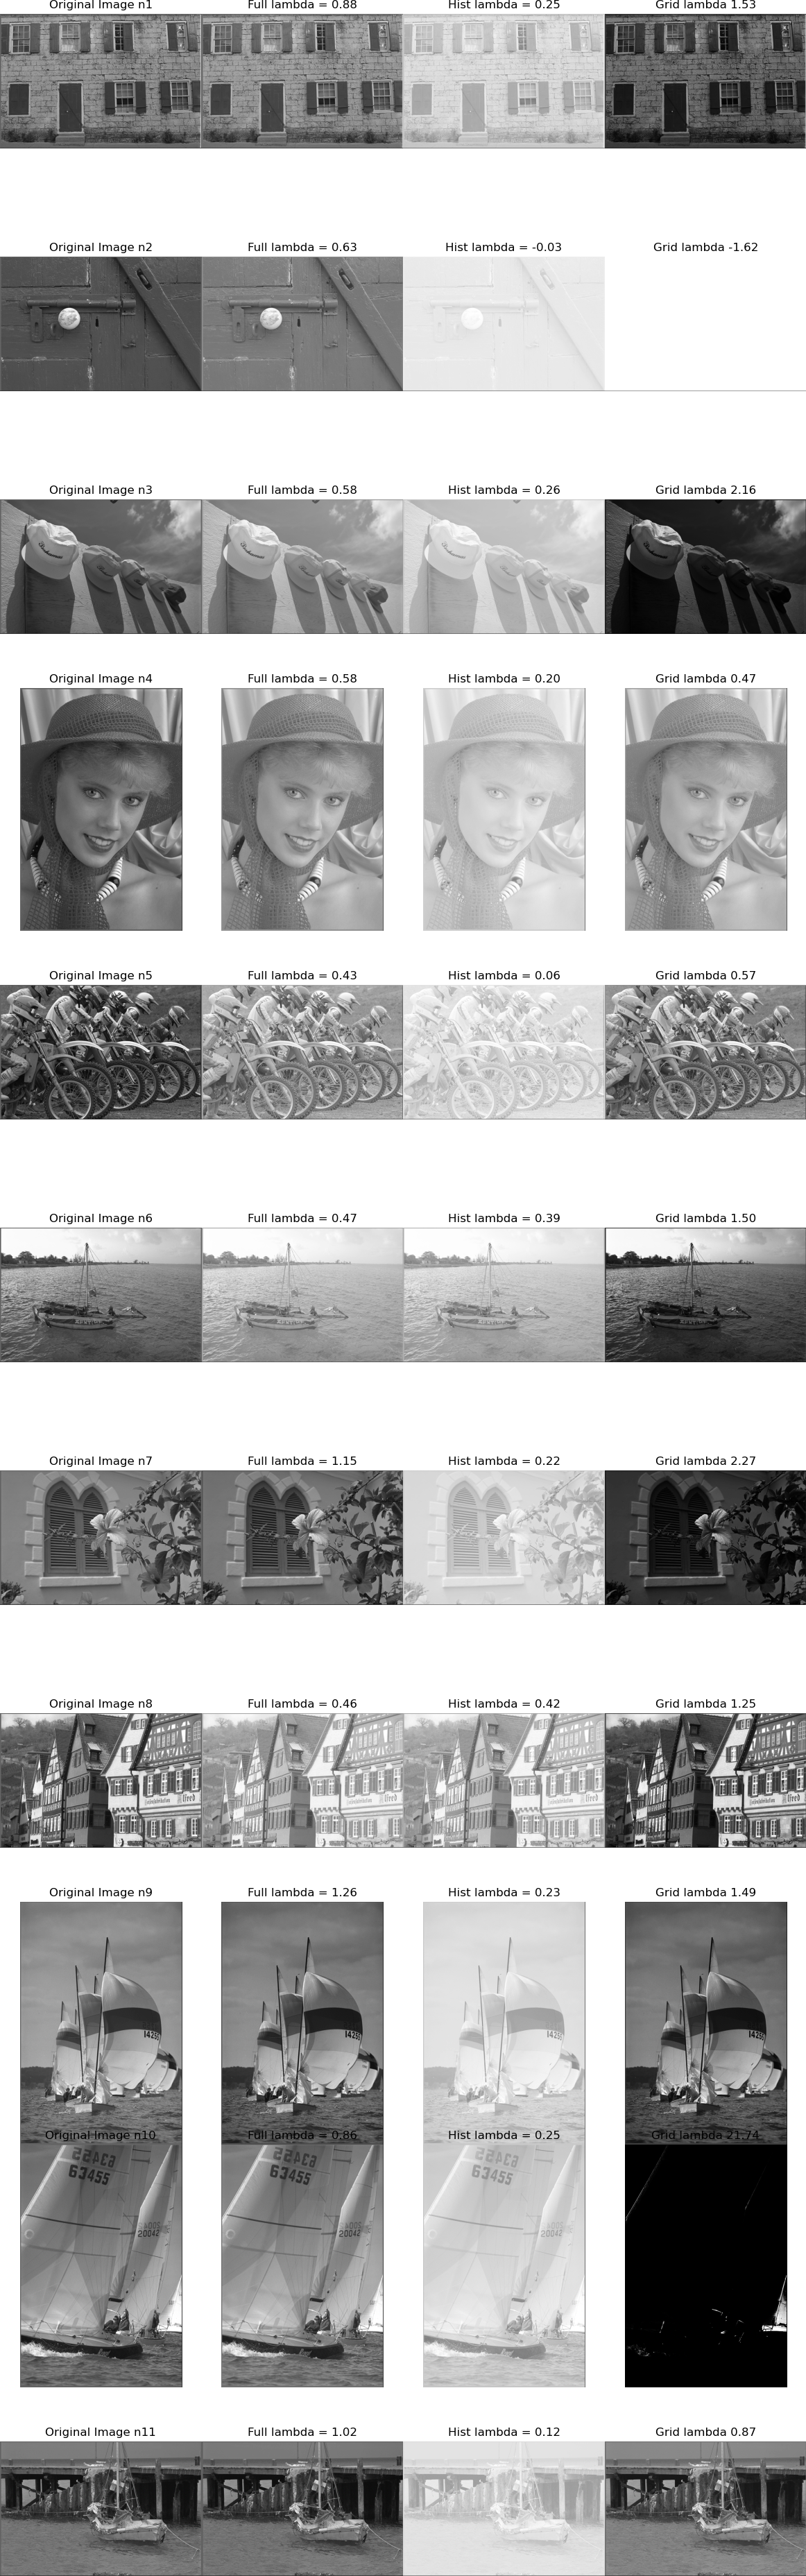
\includegraphics[width=\textwidth]{figuras/img_BCI_all_1.png}
    \caption{Imagen original junto con sus transformaci\'ones Box-Cox para los distintos m\'etodos de $\lambda$transformados, primera las im\'agenes 1 a 5.}
\end{figure}


\begin{figure}
    \centering
    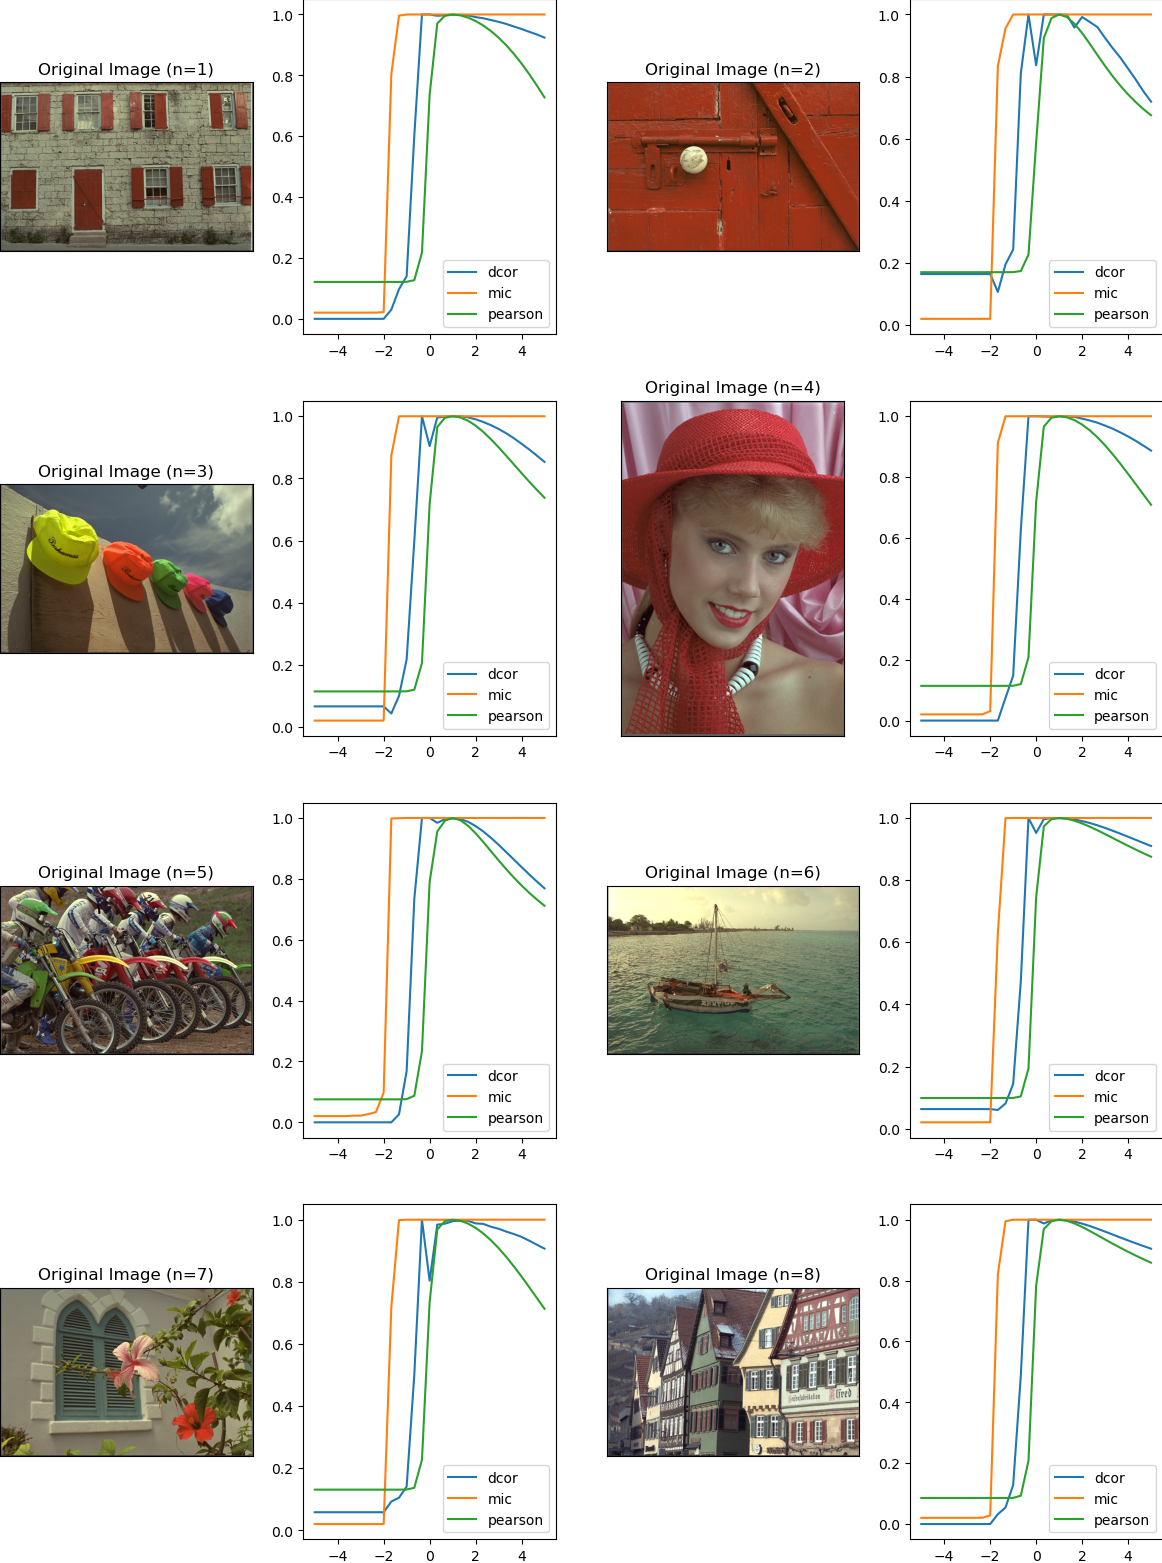
\includegraphics[width=0.8\textwidth]{figuras/full_comp_1.png}
    \caption{A la izquierda la im\'agen original y a la derecha el valor de $dCor$ (azul), $MIC$ (rojo), y $\rho$ (amarillo) utilizando el vector completo en el eje y, $\lambda$ en el eje x, imagenes 1 a 8.}
\end{figure}

\begin{figure}
    \centering
    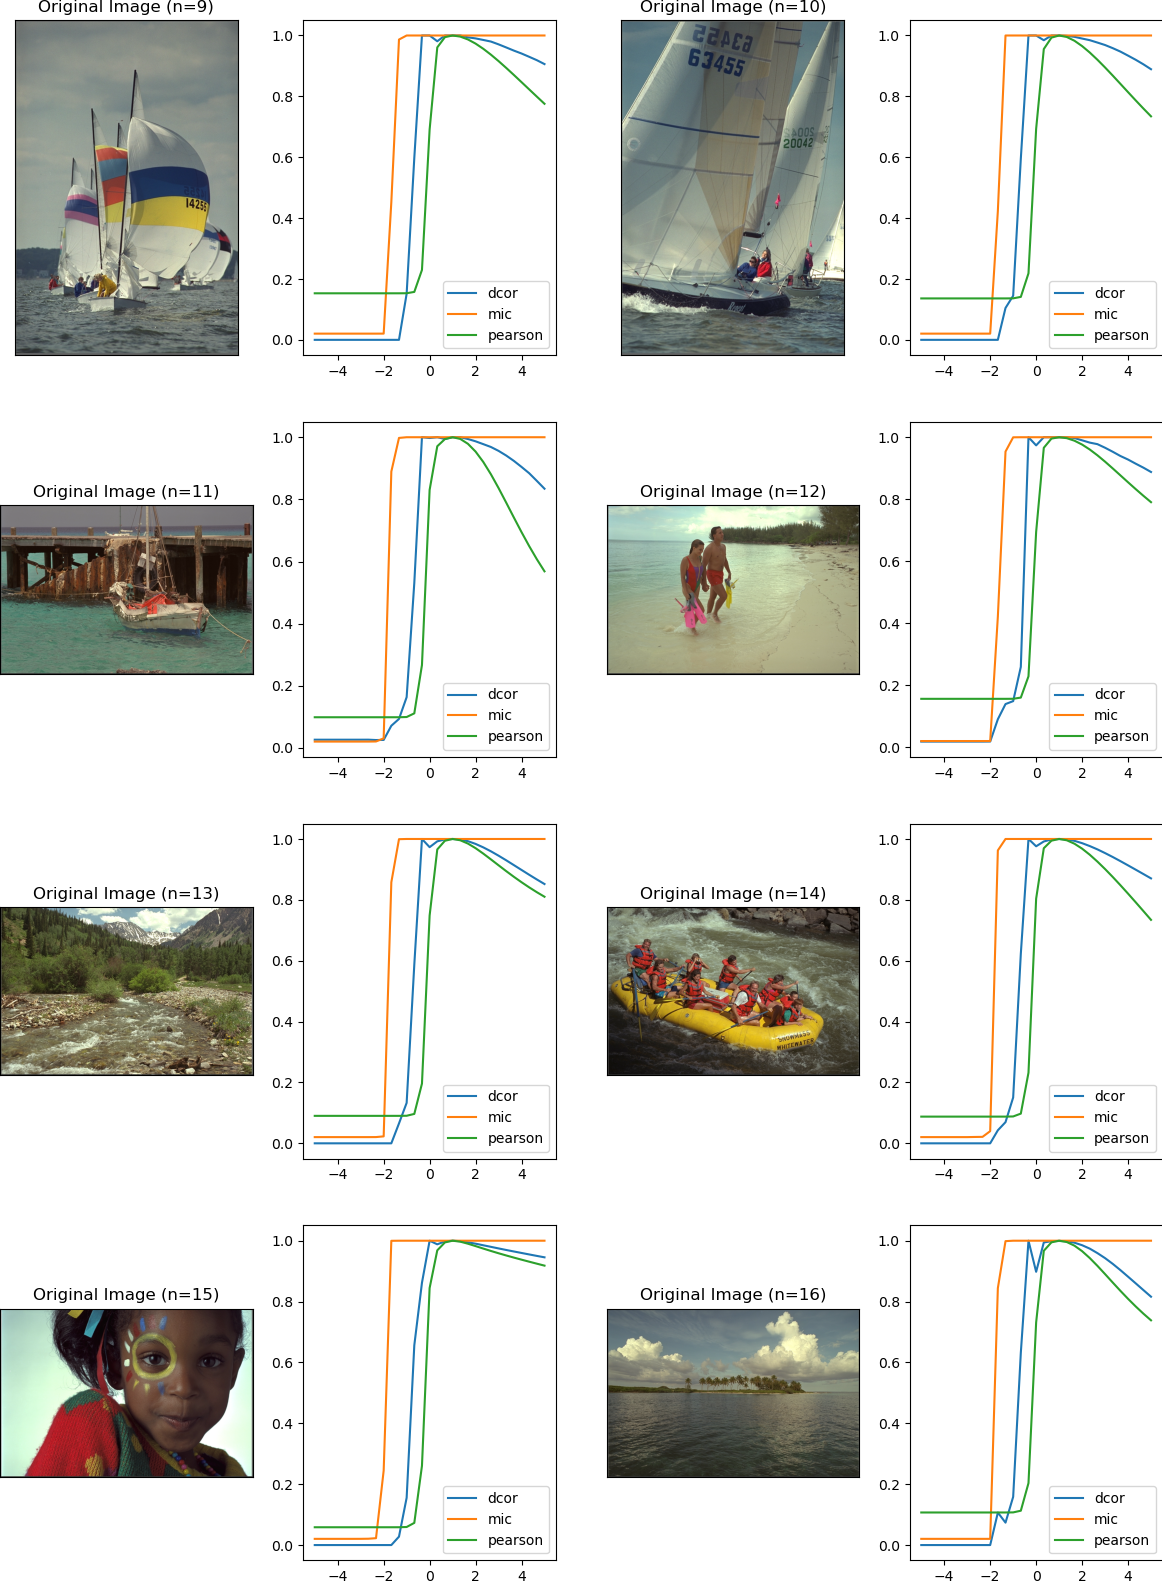
\includegraphics[width=0.8\textwidth]{figuras/full_comp_2.png}
    \caption{A la izquierda la im\'agen original y a la derecha el valor de $dCor$ (azul), $MIC$ (rojo), y $\rho$ (amarillo) utilizando el vector completo en el eje y, $\lambda$ en el eje x, imagenes 9 a 16.}
\end{figure}


\begin{figure}
    \centering
    \includegraphics[width=0.8\textwidth]{figuras/full_comp_3.png}
    \caption{A la izquierda la im\'agen original y a la derecha el valor de $dCor$ (azul), $MIC$ (rojo), y $\rho$ (amarillo) utilizando el vector completo en el eje y, $\lambda$ en el eje x, imagenes 17 a 24.}
\end{figure}

\begin{figure}
    \centering
    \includegraphics[width=0.8\textwidth]{figuras/hist_comp_1.png}
    \caption{A la izquierda la im\'agen original y a la derecha el valor de $dCor$ (azul), $MIC$ (rojo), y $\rho$ (amarillo) utilizando el histograma en el eje y, $\lambda$ en el eje x, imagenes 1 a 8.}
\end{figure}

\begin{figure}
    \centering
    \includegraphics[width=0.8\textwidth]{figuras/hist_comp_2.png}
    \caption{A la izquierda la im\'agen original y a la derecha el valor de $dCor$ (azul), $MIC$ (rojo), y $\rho$ (amarillo) utilizando el histograma en el eje y, $\lambda$ en el eje x, imagenes 9 a 16.}
\end{figure}


\begin{figure}
    \centering
    \includegraphics[width=0.8\textwidth]{figuras/hist_comp_3.png}
    \caption{A la izquierda la im\'agen original y a la derecha el valor de $dCor$ (azul), $MIC$ (rojo), y $\rho$ (amarillo) utilizando el histograma en el eje y, $\lambda$ en el eje x, imagenes 17 a 24.}
\end{figure}




% ---------------------------------------------------------------------------------------------
% ---------------------------------------------------------------------------------------
\chapter{Código.}\label{appB}

En este ap\'endice incluimos una catalogaci\'on de los c\'odigos utilizados para la realizaci\'on de este trabajo. El total de los codigos se encuentra en el repositorio de github \url{https://github.com/FabianCastellano/memoria}, junto con el \LaTeX \ de este documento, y otros archivos de interes. 

% ---------------------------------------------------------------------------------------
\chapter{Equitabilidad}\label{appC}
	En este ap\'endice distimmos a profundizar en el concepto de equitabilidad, y como podemos aplicar esta herramienta para medir la efectividad de medidas de correlaci\'on.
	\section{Introducci\'on}

	La equitabilidad ha sido descrita de manera informal por Reshef et al. como la capacidad de una estad\'istica para ''asignar puntuaciones similares a relaciones igualmente ruidosas de diferentes tipos'' \cite{Reshef2011}. Aunque \'util, esta definici\'on informal es imprecisa en el sentido de que no especifica lo que se entiende por "ruidoso" o "similar", y no especifica para qu\'e relaciones debe cumplirse la propiedad mencionada.

	En su trabajo posterior \textit{''Equitability, interval estimation, and statistical power''}, Reshef et al. (2015) \cite{Reshef2015}, se formaliz\'o la idea de Equitabilidad a travez del concepto del intervalo interpretativo, que funciona como estimaci\'on en intervalos de la cantidad de ruido presente en una relaci\'on de tipo desconocida. 

	En el contexto de este trabajo, nos interesa que las medidas de dependencia sean equitativas puesto que esto nos asegura que la medida de dependencia no est\'a sesgada hacia un tipo de relaci\'on en particular, y por lo tanto, nos ser\'a \'util para comprar comparar las distintas versi\'on de la transformac\'ion Box-Cox que definimos en la secci\'on \ref{chap4}.

	En esta secci\'on se presentar\'a la definici\'on de Intercalo Interpretativo formal, y para luego poder definir equitabilidad y  equitabilidad con respecto a $R^2$. Posteriormente, revisaremos el experimento realizado por Reshef et al. (2016) \cite{Reshef2016} sobre la equitabilidad del $MIC_e$ y $dCor$, las dos medidas definidas en \ref{chap2}. 

	\subsection[equidefiniciones]{Intervalos interpretativos.}

	Sea $\hat{\varphi}$ una estad\'istico que toma valores en el intervalo $[0,1]$, sea $\mathcal{Q}$ un conjunto de distribuciones, y sea $\Phi: \mathcal{Q} \rightarrow [0,1]$ una medida de la fuerza de la relaci\'on. Nos referimos a $\mathcal{Q}$ como el conjunto de relaciones est\'andar y a $\Phi$ como la propiedad de inter\'es. Para construir los intervalos interpretables de $\hat{\varphi}$ con respecto a $\Phi$, primero debemos preguntar cu\'anto puede variar $\hat{\varphi}$ al ser evaluado en una muestra de alguna $\mathcal{Z}$ en $\mathcal{Q}$ con $\Phi(\mathcal{Z})=x$. La siguiente definici\'on nos proporciona una forma de medir esto. (En esta definici\'on y en las definiciones en el resto de este trabajo, asumimos impl\'icitamente un tama\~o de muestra fijo de $n$.)


	\begin{defn}[Fiabilidad de un estad\'istico]
		Sea $\hat{\varphi}$ una estad\'istico que toma valores en $[0,1]$, y sean $x, \alpha \in [0,1]$. El intervalo $\alpha$-fiable de $\hat{\varphi}$ en $x$, denotado como $R_\alpha^{\hat{\varphi}}(x)$, es el intervalo cerrado m\'as peque\~no $A$ con la propiedad de que, para todas las $\mathcal{Z}$ en $\mathcal{Q}$ con $\Phi(\mathcal{Z})=x$, tenemos
		$$
		\mathbf{P}(\hat{\varphi}(Z)<\min A)<\alpha / 2 \text { and } \mathbf{P}(\hat{\varphi}(Z)>\max A)<\alpha / 2,
		$$
		
		donde $Z$ es una muestra de tama\~o $n$ de $\mathcal{Z}$.
	\end{defn}

	El estad\'istico $\hat{\varphi}$ se dice $\frac{1}{d}$-fiable con respecto a $\Phi$ en $\mathcal{Q}$ en $x$ con una probabilidad de $1-\alpha$ si y solo si el di\'ametro de $R_\alpha^{\hat{\varphi}}(x)$ es como m\'aximo $d$.
	
		
	Ver la Figura \ref{reshef_2015_f1}a para una ilustraci\'on. El intervalo confiable en $x$ es una regi\'on de aceptaci\'on de una prueba de tama\~no $\alpha$ de la hip\'otesis nula $H_0: \Phi(\mathcal{Z})=x$. Si solo hay un $\mathcal{Z}$ que satisface $\Phi(\mathcal{Z})=x$, esto equivale a un intervalo central de la distribuci\'on de muestreo de $\hat{\varphi}$ en $\mathcal{Z}$. Si hay m\'as de un $\mathcal{Z}$ que satisface esta condici\'on, el intervalo confiable se expande para incluir los intervalos centrales relevantes de las distribuciones de muestreo de $\hat{\varphi}$ en todas las distribuciones $\mathcal{Z}$ en cuesti\'on. Por ejemplo, cuando $\mathcal{Q}$ es un conjunto de relaciones funcionales ruidosas con varios tipos de funciones diferentes y $\Phi$ es $R^2$, el intervalo confiable en $x$ es el intervalo m\'as peque\~no $A$ tal que, para cualquier relaci\'on funcional $\mathcal{Z} \in \mathcal{Q}$ con $R^2(\mathcal{Z})=x$, $\hat{\varphi}(Z)$ cae en $A$ con alta probabilidad en la muestra $Z$ de tama\~no $n$ de $\mathcal{Z}$.

	Dado que el intervalo confiable $R_\alpha^{\hat{\varphi}}(x)$ se puede ver como la regi\'on de aceptaci\'on de una prueba de nivel $\alpha$ de $H_0: \Phi(\mathcal{Z})=x$, la equivalencia entre las pruebas de hip\'otesis y los intervalos de confianza proporciona estimaciones de intervalos de $\Phi$ en t\'erminos de $R_\alpha^{\hat{\varphi}}(x)$. Estos intervalos son los intervalos interpretables, definidos a continuaci\'on.

	\begin{defn}[Interpretabilidad de un estad\'istico]
		Sea $\hat{\varphi}$ un estad\'istico que toma valores en $[0,1]$, y sean $y, \alpha \in [0,1]$. El intervalo $\alpha$-interpretable de $\hat{\varphi}$ en $y$, denotado por $I_\alpha^{\hat{\varphi}}(y)$, es el intervalo cerrado m\'as peque\~no que contiene el conjunto:

		$$
		\left\{x \in[0,1]: y \in R_\alpha^{\hat{\varphi}}(x)\right\} .
		$$

		El estad\'istico $\hat{\varphi}$ es $1/d$-interpretable con respecto a $\Phi$ en $\mathcal{Q}$ en $y$ con una confianza de $1-\alpha$ si y solo si el di\'ametro de $I_\alpha^{\hat{\varphi}}(y)$ es a lo sumo $d$.
		\label{interpretabilidad}
	\end{defn}

	Ver la Figura \ref{reshef_2015_f1} para una ilustraci\'on. La correspondencia entre pruebas de hip\'otesis y estimaciones de intervalos [20] nos proporciona la siguiente garant\'ia sobre la probabilidad de cobertura del intervalo interpretable, cuya prueba omitimos.

	\begin{prop}
		Sea $\hat{\varphi}$ un estad\'istico que toma valores en $[0,1]$, y sea $\alpha \in [0,1]$. Para todo $x \in [0,1]$ y para todo $\mathcal{Z} \in \mathcal{Q}$,

		$$
		\mathbf{P}\left(\Phi(\mathcal{Z}) \in I_\alpha^{\hat{\varphi}}(\hat{\varphi}(Z))\right) \geq 1-\alpha
		$$
	\end{prop}

	Las definiciones reci\'en presentadas tienen contrapartes no estoc\'asticas naturales en el caso l\'imite de muestras grandes, que resumimos a continuaci\'on.

	\begin{defn}[Confiabilidad e interpretabilidad en el l\'imite]
		Sea $\varphi:\mathcal{Q} \rightarrow [0,1]$ una funci\'on de distribuciones. Para $x \in [0,1]$, el intervalo cerrado m\'as peque\~no que contiene el conjunto $\varphi\left(\Phi^{-1}({x})\right)$ se llama el intervalo confiable de $\varphi$ en $x$ y se denota como $R^{\varphi}(x)$. Para $y \in [0,1]$, el intervalo cerrado m\'as peque\~no que contiene el conjunto $\left\{ x: y \in \R^{\varphi} (x) \right\}$ se llama el intervalo interpretable de $\varphi$ en $y$ y se denota como $I^{\varphi}(y)$.

	\end{defn}

	Mira la Figura \ref{reshef_2015_f1}b para una ilustraci\'on.

	\begin{figure}[H] 
		\centering
		\includegraphics[scale = 0.4]{reshef_2015_fig1.png}
		\caption{
			\label{reshef_2015_f1}
			Una ilustraci\'on esquem\'atica de intervalos confiables e interpretables. En ambas partes de la figura, $\mathcal{Q}$ consiste en relaciones ruidosas de tres tipos diferentes representados en tres colores distintos. (a) La relaci\'on entre un estad\'istico $\hat{\varphi}$ y $\Phi$ en $\mathcal{Q}$ en un tama\~no de muestra finito. Los l\'imites inferior y superior de cada regi\'on sombreada indican los percentiles $(\alpha / 2) \cdot 100 \%$ y $(1 - \alpha / 2) \cdot 100 \%$ de la distribuci\'on de muestreo de $\hat{\varphi}$ para cada tipo de relaci\'on en varios valores de $\Phi$. El intervalo vertical (en negro) es el intervalo confiable $R_\alpha^{\hat{\varphi}}(x)$, y el intervalo horizontal (en rojo) es el intervalo interpretable $I_\alpha^{\hat{\varphi}}(y)$. (b) En el l\'imite de muestra grande, reemplazamos $\hat{\varphi}$ por una cantidad poblacional $\varphi$. El intervalo vertical (en negro) es el intervalo confiable $R^{\varphi}(x)$, y el intervalo horizontal (en rojo) es el intervalo interpretable $I^{\varphi}(y)$.}
	\end{figure}

	\section{Definiendo Equitabilidad}

	La proposici\'on \ref{interpretabilidad} implica que si los intervalos de interpretabilidad de $\hat{\varphi}$ con respecto a $\Phi$ son pequen\~os, entonces $\hat{\varphi}$ dar\'a buenos intervalos de estimac\'on de $\Phi$. Hay variadas formas de resumir si los intervalos de interpretabilidad son peque\~nos; nos enfocaremos en dos formas simples de hacerlo.
	
	\begin{defn}[$\alpha$-fiabilidad y $\alpha$-interpretabilidad]
		La \textit{$\alpha$-fiabilidad (resp. $\alpha$-interpretabilidad) en caso peor} de $\hat{\varphi}$ es $1/d$ si es $1/d$-fiable (resp. interpretable) para todo $x$ (resp. $y$) $\in [0,1]$. Se dice que $\hat{\varphi}$ es \textit{$1/d$-fiable (resp. $\alpha$-interpretable) en caso peor} con probabilidad (resp. confianza) $1-\alpha$.

		La \textit{$\alpha$-fiabilidad (resp. $\alpha$-interpretabilidad) en caso promedio} de $\hat{\varphi}$ es $1/d$ si su fiabilidad (resp. interpretabilidad), promediada sobre todo $x$ (resp. $y$) $\in [0,1]$, es al menos $1/d$. Se dice que $\hat{\varphi}$ es \textit{$1/d$-fiable (resp. $\alpha$-interpretable) en caso promedio} con probabilidad (resp. confianza) $1-\alpha$
	\end{defn}

	Con este vocaculario, podemos definir equitabilidad.

	\begin{defn}
		La \textit{Equitabilidad en caso promedio/peor} es simplemente \textit{interpretabilidad en caso promedio/peor} con respecto a un $\Phi$ que refeleje la fuerza de la relaci\'on. 
	\end{defn}

	\begin{rem}
		Notemos que Equitabilidad es un caso en particular de interpretabilidad donde $\Phi$ cumple un rol en especifico. Es posible definir un $\Phi$ que mida otras propiedades y resalte otro tipo de relaci\'ones. En este trabajo usaremos $R^2$ para medir fuerza entre relaciones, ahondaremos m\'as en esto en la siguiente secci\'on.
	\end{rem}

	Las definiciones correspondientes de interpretabilidad/fiablidad en caso promedio/peor son posibles para $\varphi$ in el caso de l\'imite para muestras grandes. En este caso, es posible que todos los intervalos de interpretabilidad de $\varphi$ con respecto a $\Phi$ tengan taman\~o 0, esto es, que el valor de $\varphi(Z)$ determina \'unicamente el valor de $\Phi(Z)$. En este caso, la interpretabilidad/fiablidad en caso promedio/peor de $\varphi$ es $\infty$, y se dice que $\varphi$ es perfectamente interpretable/fiable, o perfectamente equitativo dependiendo del contexto.

	Antes de seguir con la siguiente secci\'on, con el objetivo de construir intuici\'on, vamos a presentar dos ejemplos de estadi\'isticos que son perfectamente interpretables en el caso 
	l\'imite para muestras grandes. Primero, la Informaci\'on M\'utua \cite{CoverThomas2006}\cite{inftheo2008} es perfectamente interpretable con respecto a la correlaci\'on $\rho^2$ en el conjunto $\mathcal{Q}$ de vectores normales bivariados. Esto es dado que para normales bivariadas tenemos que $1-2^{-2I} = \rho^2$ \cite{infcorr}. Adicionalmente, el Teorema 6 de \cite{Szekely2009} muestra que para normales bivariadas, la correlaci\'on por distancia es tambi\'en es una funci\'on completamente determinada por $\rho^2$. Por lo tanto, la correlaci\'on por distancia tambi\'en es perfectamente interpretable y perfectamentef fiable con respecto a $\phi^2$ en el conjunto normales bivariadas $\mathcal{Z}$.

	La interpretabilidad perfecta con respecto a $\rho^2$ en bivariadas normales exhibida en ambos ejemplos es de hecho equivalente a una de las ''propiedades fundamentales'' introducidas por R\'enyi en su m\'etodo para evaluar las propiedades ideales de medidas de dependencia \cite{renyi1959}. Esto contiene un compromiso: Por un lado garantiza interpretabilidad perfecta, pero por el otro, solo aplica en un conjunto de relaciones relativamente pequen\~o. Uno de los objetivo de la Equitabilidad es relajar el requermiento de ''perfecci\'on'' a cambio de la habilidad de aplicar a un conjunto de relaciones m\'as amplio, por ejemplo, un conjuntod e funcionales ruidosos. Por tanto, es posible ver la equitabilidad como una generalizaci\'on de los requermiento de R\'enyi que nos permite hacer un intercambio entre la precisi\'on con la que nuestro estad\'istico nos informa sobre $\Phi$ y el conjunto $\mathcal{Q}$ sobre el cu\'al act\'ua.
	
	\section[Interpretabilidad sobre r2]{Interpretabilidad sobre $R^2$}

	Durante este cap\'itulo hemos mencionado el concepto de relaciones funcionales ruidosas y de $R^2$, ahora los definimos de forma formal. Comenzemos primero con $R^2$
	\begin{defn}[$R^2$]
		Sea $y=[y_1,\dots,y_n]\in\R^n$ un vector de muestras de una variable aleatoria y sea $f:\R\to\R$ una funci\'on que modela la variable aleatoria, definamos $f_i:=f(y_i)$. El coeficiente de determinaci\'on o $R^2$ se define como:

		$$
		R^2 = 1 - \frac{\sum_i(y_i-f_i)^2}{\sum_i(y_i-\bar{y})^2},
		$$

		donde $\sum_i(y_i-f_i)^2$ corresponde a la suma del cuadrado de los residuales, $\sum_i(y_i-\bar{y})^2$ es la suma total de cuadrados (proporcional a la varianza), e $\hat{y}$ es el promedio de la muestra.
	\end{defn}

	En palabras simples, $R^2$ es la proporci\'on de variaci\'on en la variable dependiente que puede ser explicado por la variable independiente. Notemos que al momento de hacer el an\'alisis de equitabilidad, tenemos total claridad de cual es nuestra funci\'on $f$, dado que nosotros definimos la relaci\'on. Veamos ahora la siguiente definici\'on.	
		
	\begin{defn}[Relaci\'on Funcional Ruidosa]
		Una variable aleatoria distribuida sobre $\R^2$ es llamada una \textit{relaci\'on funcional ruidosa} si, y solo si, puede ser escrita en la forma $(X+\epsilon, f(X)+\epsilon\prime)$, donde $f:[0,1]\to\R$, $X$ es una variable aleatoria distribuida sobre $[0,1]$, y $\epsilon$ y $\epsilon\prime$ son (posiblemente nulas) distribuciones aleatorias. Denotamos el conjunto de todas las relaciones funcionales ruidosas como $\mathcal{F}$
		\label{ruido_func}
	\end{defn}

	Ya con esto, tenemos todo lo que necesitamos para definir la equitabilidad que usaremos para los an\'alisis de la siguiente secci\'on: Equitabilidad sobre $R^2$

	\begin{defn}[Equitabilidad en relaciones funcionales sobre $R^2$]
		Sea $\mathcal{Q}\in\mathcal{F}$ un conjunto de relaciones funcionales ruidosas. Una medida de dependencia es $1/d$-equitativa en $\mathcal{Q}$ con respecto a $R^2$ si es $1/d$-interpretable sobre $R^2$ en $\mathcal{Q}$ 
	\end{defn}

	Es necesario destacar que esta definici\'on aun depende del conjunto $\mathcal{Q}$ en cuesti\'on. El m\'etodo generalmente utilizado en la literatura ha sido fijar un conjunto $F$ de funciones tales que sean lo suficientemente grandes como para ser representativo de las relaciones encontradas en datos reales, pero que por otro lado sean lo suficientemente pequen\~nos tal que permitan an\'alsis emp\'irico. Discutiremos el $F$ a ultilziar en la siguiente secci\'on, donde realizaremos un ana\'alisis de equitabilidad sobre los estad\'isticos definidos en este trabajo.

	Tan importante como la elecc\'ion de funciones a incluir en $F$, es la elecci\'on de distribuciones marginales y el ruido, los cuales fueron no son especificados en la definici\'on \ref{ruido_func}. Varias posibilidades han sido propuestas por Reshef et al. \cite{Reshef2015a}, pero la m\'as utilizada en la literatura, y la que usaremos en la siguiente secci\'on, continua siendo la m\'as simple con $X\sim Unif$, $\epsilon\prime\sim\mathcal{N}(0,\sigma^2)$ con $\sigma$ variable y $\epsilon\equiv0$. 

	
	\section{Equitabilidad de las medidas}
	
	Como se mencion\'o previamente, una de las principales motivaciones para la introducci\'on de $MIC$ fue la equidad, es decir, hasta qu\'e punto una medida de dependencia captura \'utilmente alguna noci\'on de la fuerza de una relaci\'on en un conjunto de relaciones est\'andar. En esto contexto en Reshef et al. (2016) \cite{Reshef2016} se realiz\~o un an\'alisis emp\'irico de la equidad de $MIC_e$ con respecto a R2 y su desempe\~no fue comparado con la correlaci\'on de distancia (Sz\'ekely et al., (2007)\cite{Szekely2007}; Sz\'ekely and Rizzo, (2009)\cite{Szekely2009}), la estimaci\'on de la informaci\'on mutua (Kraskov et al., 2004) y la estimaci\'on de la correlaci\'on m\'axima (Breiman and Friedman, 1985).

	Se comenz\'o evaluando la equidad en el conjunto de relaciones $Q$ definido anteriormente, un conjunto que ha sido analizado en otros trabajos previos (Reshef et al., 2011, 2015a; Kinney and Atwal, 2014). Los resultados, mostrados en la Figura \ref{reshef_2016_f3}, confirman la superior equidad del estimador $MIC_e$ en este conjunto de relaciones.

	Para evaluar la equidad de manera m\'as objetiva sin depender de un conjunto de funciones curado manualmente, se analizaron 160 funciones aleatorias extra\'idas de una distribuci\'on de proceso Gaussiano con un kernel de funci\'on radial con una de ocho posibles anchuras en el conjunto $\{0.01, 0.025, 0.05, 0.1, 0.2, 0.25, 0.5, 1\}$ para representar una variedad de complejidades de relaciones posibles. Los resultados, mostrados en la Figura \ref{reshef_2016_f4}, muestran que $MIC_e$ supera a los m\'etodos existentes en t\'erminos de equidad con respecto a $R^2$ en estas funciones tambi\'en. Tambi\'en se examin\'o el efecto de las relaciones at\'ipicas en los resultados al muestrear repetidamente subconjuntos aleatorios de 20 funciones de este gran conjunto de relaciones y medir la equidad de cada m\'etodo en promedio sobre los subconjuntos; los resultados fueron similares.

	Una caracter\'istica del desempe\~no de $MIC_e$ en estas relaciones elegidas al azar, como se muestra en la Figura \ref{reshef_2016_f4}, es que parece ser m\'inimamente sensible a la anchura del proceso Gaussiano del cual se extrae una relaci\'on dada. Esto contrasta, por ejemplo, con la estimaci\'on de la informaci\'on mutua, que muestra una sensibilidad pronunciada a este par\'ametro que le impide ser altamente equitativa cuando hay relaciones con diferentes anchuras en el mismo conjunto de datos.

	\begin{figure}[H] 
		\centering
		\includegraphics[scale = 0.4]{reshef_2016_fig3.png}
		\caption{Equitabilidad con respecto a $R^2$ en un conjunto de relaciones funcionales ruidosas de $(a)$ el coeficiente de correlaci\~on de Pearson, $(b)$ una medida hipot\~etica de dependencia $\varphi$ con equitabilidad perfecta, $(c)$ la correlaci\~on de distancia, $(d)$ $\mathrm{MIC}_e$, $(e)$ estimaci\~on de correlaci\~on m\~axima y $(f)$ estimaci\~on de informaci\~on mutua. Para cada relaci\~on, una regi\~on sombreada denota los valores estimados en el percentil 5 y 95 de la distribuci\~on muestral de la estad\~istica en cuesti\~on en esa relaci\~on en cada valor de $R^2$. El gr\~afico resultante muestra qu\~e valores de $R^2$ corresponden a un valor dado de cada estad\~istica. El intervalo rojo en cada gr\~afico indica el rango m\~as amplio de valores de $R^2$ que corresponden a un valor de la estad\~istica; cuanto m\~as estrecho sea el intervalo rojo, mayor ser\~a la equitabilidad. Un intervalo rojo con ancho 0, como en $(b)$, significa que la estad\~istica refleja solo $R^2$ sin depender del tipo de relaci\~on, como se demuestra en los pares de miniaturas de relaciones de diferentes tipos con valores id\~enticos de $R^2$.}
		\label{reshef_2016_f3}
	\end{figure}

	\begin{figure}[H] 
		\centering
		\includegraphics[scale = 0.4]{reshef_2016_fig4.png}
		\caption{Equitabilidad de los m\~etodos examinados en funciones extra\~idas al azar de una distribuci\~on de proceso gaussiano. Cada m\~etodo se eval\~ua como se muestra en la Figura \ref{reshef_2016_f3}, con un intervalo rojo que indica el rango m\~as amplio de valores de $R^2$ correspondiente a cualquier valor de la estad\~istica; cuanto m\~as estrecho sea el intervalo rojo, mayor ser\~a la equitabilidad. Cada regi\~on sombreada corresponde a una relaci\~on, y las regiones est\~an coloreadas seg\~un el ancho de banda del proceso gaussiano del que se muestrearon. Las relaciones de muestra para cada ancho de banda se muestran en la esquina superior derecha con colores correspondientes.}
		\label{reshef_2016_f4}
	\end{figure}


% ---------------------------------------------------------------------------------------------

\blankpage
\printbibliography %Prints bibliography
% --------------------------------------------------
\end{document} 